\documentclass[lang=cn,11pt]{elegantbook}

\title{离散数学}
\subtitle{期末备考复习笔记}

\author{夏同}
\institute{}
\date{\today}
\version{1.0}

\setcounter{tocdepth}{2}

\usepackage{amsmath,amssymb,bm,mathrsfs}
\allowdisplaybreaks
\usepackage{array}
\usepackage{enumitem}
\setlist{itemsep=-1pt}
\setlist[enumerate]{itemsep=-1pt, parsep=-1pt, topsep=0pt}
\usepackage{graphicx}
\usepackage{pgfplots}
\pgfplotsset{compat=1.18}
\usepackage{tikz}
\usepackage{circuitikz}
\usetikzlibrary{arrows,shapes.geometric,circuits.logic.US,positioning}
\usepackage{ulem}
\usepackage{caption}
\usepackage{cleveref}

\graphicspath{{./learn-lisanshuxue/flg/}{./learn-lisanshuxue/}{./figure/}{./image/}}

\newcommand{\R}{\mathbb{R}}
\newcommand{\C}{\mathbb{C}}
\newcommand{\Z}{\mathbb{Z}}
\newcommand{\N}{\mathbb{N}}
\newcommand{\e}{\text{e}}
\newcommand{\dd}{\text{d}}
\newcommand{\nothing}{\ensuremath{\varnothing}}
\newcommand{\kt}{\kaishu}
\newcommand{\st}{\songti}
\newcommand{\htbf}{\heiti\bfseries}

\makeatletter
\@ifundefined{setCJKfamilyfont}{}{%
  \IfFontExistsTF{KaiTi}{%
    \setCJKfamilyfont{codexkaiti}[AutoFakeBold=2.5]{KaiTi}%
    \renewcommand{\kaishu}{\CJKfamily{codexkaiti}}%
  }{}%
  \IfFontExistsTF{FangSong}{%
    \setCJKfamilyfont{codexfangsong}[AutoFakeBold=2.5]{FangSong}%
    \renewcommand{\fangsong}{\CJKfamily{codexfangsong}}%
  }{}%
}
\makeatother

\sloppy

\begin{document}

\maketitle
\frontmatter\chapter*{前言}
\addcontentsline{toc}{chapter}{前言}

离散数学作为计算机科学的基础核心课程，涵盖逻辑、集合、关系、图论等众多重要概念。这些抽象的理论不仅是后续课程（如数据结构、算法、数据库、编译原理）的基石，更是培养计算思维和形式化推理能力的关键。

为帮助同学们更好地复习和掌握本课程的核心内容，特编写此份学习笔记。笔记以华南理工大学计算机科学与工程学院使用的《离散数学及其应用》（陈琼，马千里等编著）为主要参考，结合课堂讲授和个人理解，对知识点进行了系统梳理和归纳。

首先感谢陈琼、马千里等老师编著的优秀教材，为学习离散数学提供了系统而全面的框架。同时感谢学院老师们的悉心讲授，使我能够理解并掌握这些抽象概念。

由于本人学识有限，笔记中难免存在疏漏、错误或不妥之处。恳请各位读者不吝指正。期望这份笔记能够为同学们的期末复习提供些许帮助。

\vspace{0.5cm}
\begin{flushright}
夏同\\
于华南理工大学\\
\today
\end{flushright}

% 目录

\tableofcontents

\mainmatter
% ===== Copied from learn-lisanshuxue/chapters/chap1.tex =====
\chapter{命题逻辑}
\section{命题与命题公式}
\begin{definition}{命题}
    命题是用陈述句表示的一个为真或者为假，但不能同时为真又为假的判断语句
\end{definition}
一个语句是命题，关键在于它是否在“逻辑上”具有一个确定的真值（即要么为真，要么为假），而不取决于我们是否知道或能够验证这个真值。只要一个陈述句在原则上可能为真或为假，即使我们目前无法判断（例如由于科学限制或信息不足），它仍然是一个命题。

比如“除了地球以外的其他星球有生物”，好像我们还不知道真假，但是我们知道，它有一个潜在的真值：要么其他星球上存在生物（真），要么不存在（假）。尽管我们目前无法证实或证伪这个陈述，但它的真值是客观存在的，不会同时为真又为假。

而语句“$2+x=5$”，我们从逻辑上无法认为它一定为真，或者一定为假，因为$x$是变元，有时这个式子成立，有时不成立，因此这个语句不是命题。

除此以外，问句，感叹句，祈使句表示的语义不具备真值，不是命题。比如“多漂亮的花啊！”这句话，有的人觉得好看，有的人觉得不好看，所以它没有确定的真值，不是命题。
\begin{definition}{悖论}
悖论是用陈述句表示的一个如果为真则推出为假、如果为假则推出为真，从而无法一致地分配真值的判断语句。
\end{definition}
例如著名的理发师悖论。
\begin{definition}{原子命题（简单命题）}
原子命题是不能被分解为更简单命题的命题，它不包含任何逻辑联结词，是构成复合命题的基本单位。
\end{definition}
原子命题（简单命题）的特点是它的真值是内在的、最基本的，不依赖于其他命题。例如：“今天是星期五。”和“雪是白的。”
\begin{definition}{复合命题}
复合命题是由一个或一个以上的原子命题（简单句）通过逻辑联结词（如“并非”、“并且”、“或者”、“如果…那么…”、“当且仅当”等连词）组合而成的命题。
\end{definition}
复合命题的真值则完全由其包含的原子命题的真值以及所使用的逻辑联结词的规则共同决定。例如：“今天是星期五并且天气很好。” 这个复合命题的真假，取决于“今天是星期五”和“天气很好”这两个原子命题的真假以及“并且”这个词的逻辑含义。
\begin{definition}{逻辑联结词}
    逻辑联结词是用来连接一个或多个命题，从而构成更复杂的复合命题的逻辑运算符。它们定义了原子命题之间的逻辑关系，并决定了复合命题的真值。\\
    1. \textbf{否定联结词}（$\neg$，读作"非"）：表示对原命题的否定。命题 $\neg P$ 为真，当且仅当命题 $P$ 为假。\\
    2. \textbf{合取联结词}（$\land$，读作"且"或"与"）：表示两个命题同时成立。命题 $P \land Q$ 为真，当且仅当 $P$ 和 $Q$ 同时为真。\\
    3. \textbf{析取联结词}（$\lor$，读作"或"）：表示两个命题至少有一个成立。命题 $P \lor Q$ 为真，当且仅当 $P$ 和 $Q$ 至少有一个为真（此为"相容或"，即允许两者同时为真）。\\
    4. \textbf{蕴涵联结词}（$\rightarrow$ 或 $\supset$，读作"如果…那么…"）：表示前一个命题是后一个命题的充分条件。命题 $P \rightarrow Q$ 为假，当且仅当 $P$ 为真而 $Q$ 为假；其余情况均为真。\\
    5. \textbf{等价联结词}（$\leftrightarrow$，读作"当且仅当"）：表示两个命题互为充分必要条件。命题 $P \leftrightarrow Q$ 为真，当且仅当 $P$ 和 $Q$ 的真值相同（即同真或同假）。\\
    6. \textbf{与非联结词}（$\uparrow$，读作"与非"）：表示合取的否定。命题 $P \uparrow Q$ 为真，当且仅当 $P$ 和 $Q$ 不同时为真。其真值等价于 $\neg(P \land Q)$。\\
    7. \textbf{或非联结词}（$\downarrow$，读作"或非"）：表示析取的否定。命题 $P \downarrow Q$ 为真，当且仅当 $P$ 和 $Q$ 同时为假。其真值等价于 $\neg(P \lor Q)$。\\
    8. \textbf{异或联结词}（$\oplus$，读作"异或"）：表示不相容的析取。命题 $P \oplus Q$ 为真，当且仅当 $P$ 和 $Q$ 的真值不同（即一真一假）。其真值等价于 $(P \land \neg Q) \lor (\neg P \land Q)$。
\end{definition}
比如“登录服务器必须输入一个有效的口令”，符号化后就是：令 $P$ 表示“登录服务器”，令 $Q$ 表示“输入一个有效的口令”，则该命题可符号化为 $P \rightarrow Q$。需要注意的是，后者只是必要条件而不是充分条件，因为输入口令后，可能还需要其他步骤才能登录服务器。

有的人不理解的可能是为什么蕴含前件为假时，蕴含式总为真。这个定义源于我们对“承诺”或“规则”是否被违反的判断。逻辑学中的蕴涵式 $P \rightarrow Q$ 可以看作一个“承诺”：\textbf{如果 $P$ 成立，则我保证 $Q$ 也成立。} 这个承诺的真假，取决于在 $P$ 成立的情况下，我是否履行了承诺。如果 $P$ 是假的，那么前提条件就没有被满足，这个规则或承诺就自动进入“不适用”或“未被激活”的状态。既然承诺没有被激活，那么我们自然不能说它被违反了。在逻辑上，我们便将“未被违反”的状态定义为“真”。
\begin{definition}{逻辑联结词的运算优先级}
    $\neg> \land> \lor> \rightarrow> \leftrightarrow$，合取优先级大于析取优先级。
\end{definition}
给定一个含有$n$个命题变元的命题公式，易得这$n$个命题变元共有$2^n$种不同的赋值，将命题公式在所有赋值下的真值列成一个表，称为该命题的真值表，所以真值表有$2^n$行，真值表实际上定义了一个函数，从 $2^n$种赋值映射到一个真值 (真或假)。对于每种赋值，函数的输出可以是真或假两种选择。因此，所有可能的函数数量是$2^{2^n}$个。这意味着，对于n个命题变元，存在$2^{2^n}$个不同的真值表。
\begin{definition}{（最小）全功能联结词集}
    在命题逻辑中，一个联结词集合被称为\textbf{全功能联结词集}，当且仅当该集合中的联结词足以表达所有可能的真值函数。换句话说，使用该集合中的联结词可以构造出任意的命题公式，并能够表示所有可能的$2^{2^n}$个不同的真值表（其中$n$为命题变元的个数）。如果从一个全功能联结词集中移除任何一个联结词后，剩下的联结词集合不再是全功能的，则称该集合为\textbf{最小全功能联结词集}。
\end{definition}
常见的最小全功能联结词集有：$\{\neg, \land\}$，$\{\neg, \lor\}$，$\{\neg, \rightarrow\}$，$\{\uparrow\}$ （与非集），$\{\downarrow\}$ （或非集）。考试一般考选择题，归纳出特点就是：联结词集必须能够表达否定；常见题型中通常显式含有$\neg$，或者由$\uparrow,\downarrow$等联结词隐含提供否定能力。析取、合取、蕴含这三个出现一个通常就够，不出现时可能是单一的$\{\uparrow\}$ （与非集），$\{\downarrow\}$ （或非集）。

\textbf{特别的，异或$\{\oplus\}$不是最小全功能联结词集，甚至不是全功能联结词集。}事实上，命题的真值只有0和1，而恰好异或运算有一个重要特性：当输入的真值变化时，输出总是以"可预测的线性方式"变化。具体来说，如果我们只使用异或运算，无论怎么组合，得到的结果都只能表达"奇偶校验"类型的关系——即计算输入中1的个数是奇数还是偶数。这种运算无法表达更复杂的逻辑关系，比如"两个输入必须同时为1"（与运算）或"至少一个输入为1"（或运算）。

为什么与运算和或运算更强大呢？因为它们能表达"非线性"的关系。与运算$P \land Q$要求两个输入必须同时满足条件，这不是简单的奇偶关系。同样，或运算$P \lor Q$允许至少一个条件满足，这也超出了异或的能力范围。

而与非运算$\uparrow$和或非运算$\downarrow$之所以强大，是因为它们内在包含了"否定"的能力。例如，单用与非运算就能表示否定：$\neg P = P \uparrow P$。一旦能够表示否定，再加上它们原有的组合能力，就可以构造出所有其他逻辑运算，包括与、或、蕴含等。
\begin{example}
联结词集 $\{\oplus, \rightarrow\}$ 是最小全功能联结词集。
\end{example}
\begin{solution}
1. 全功能性证明。
已知 $\{\neg, \rightarrow\}$ 是全功能集，因为
\[
P \land Q \equiv \neg(P \rightarrow \neg Q), \quad
P \lor Q \equiv \neg P \rightarrow Q.
\]
因此，只需证明用 $\oplus$ 和 $\rightarrow$ 可以表示 $\neg$。注意到 $P \oplus P$ 是永假式（因为 $P$ 与自身相同时异或结果为假）。考虑公式
\[
P \rightarrow (P \oplus P).
\]
当 $P$ 为真时，$P \oplus P$ 为假，于是 $P \rightarrow \text{假}$ 为假；当 $P$ 为假时，蕴含式 $P \rightarrow \text{假}$ 为真。所以
\[
\neg P \equiv P \rightarrow (P \oplus P).
\]
因此 $\neg$ 可由 $\{\oplus, \rightarrow\}$ 表示。由于 $\rightarrow$ 已在集合中，故 $\{\oplus, \rightarrow\}$ 可以模拟 $\{\neg, \rightarrow\}$，从而是全功能的。
\\2. 极小性证明：需验证 $\{\oplus\}$ 和 $\{\rightarrow\}$ 单独都不是全功能的。

$\{\oplus\}$ 不是全功能的：考虑只由 $\oplus$ 和命题变元构成的公式。对任意赋值，公式的真值等于各变元真值的“奇偶和”（即模2加法）。具体来说，每个变元出现奇数次时会影响结果，出现偶数次时不影响。但并非所有布尔函数都能写成这种形式。例如，合取 $P \land Q$ 就无法用 $\oplus$ 表示。因为假设存在由 $\oplus$ 构成的公式 $\varphi(P,Q)$ 等价于 $P \land Q$，则 $\varphi$ 的真值表应满足：当 $(P,Q)=(0,0),(0,1),(1,0)$ 时 $\varphi$ 为假，$(1,1)$ 时 $\varphi$ 为真。但在两个变元 $P,Q$ 的真值表上，只由 $\oplus$ 构成的非零线性式成真赋值数为2，零式成真赋值数为0；而 $P \land Q$ 的真值表中只有一个赋值使其为真，矛盾。所以 $\{\oplus\}$ 不能表示 $P \land Q$，从而不是全功能的。

 $\{\rightarrow\}$ 不是全功能的：考虑只由 $\rightarrow$ 和命题变元构成的公式。当所有命题变元都赋值为真时，公式的真值也一定为真。这是因为：如果 $A$ 和 $B$ 都为真，则 $A \rightarrow B$ 为真；归纳可知，任何只含 $\rightarrow$ 的公式在所有变元为真时必真。但否定 $\neg P$ 在所有变元为真（即 $P$ 为真）时为假，所以 $\neg P$ 不能用一个在所有变元为真时也为真的公式表示。因此 $\{\rightarrow\}$ 不能表示否定，从而不是全功能的。

综上，$\{\oplus, \rightarrow\}$ 是全功能的，且去掉其中任何一个联结词后都不再全功能，故为最小全功能联结词集。
\end{solution}
\begin{example}
    证明$\{\uparrow\}$ （与非集），$\{\downarrow\}$ （或非集）是最小全功能联结词集
\end{example}
\begin{solution}
\begin{align*}
    \neg P &\Leftrightarrow P \uparrow P &
    P \land Q &\Leftrightarrow (P \uparrow Q) \uparrow (P \uparrow Q) \\
    P \lor Q &\Leftrightarrow (P \uparrow P) \uparrow (Q \uparrow Q) &
    P \rightarrow Q &\Leftrightarrow P \uparrow (Q \uparrow Q) \\
    P \leftrightarrow Q &\Leftrightarrow \Bigl(\bigl(P \uparrow (Q \uparrow Q)\bigr) \uparrow \bigl(Q \uparrow (P \uparrow P)\bigr)\Bigr) \\
    &\qquad \uparrow \Bigl(\bigl(P \uparrow (Q \uparrow Q)\bigr) \uparrow \bigl(Q \uparrow (P \uparrow P)\bigr)\Bigr)
\end{align*}
类似地：
\begin{align*}
    \neg P &\Leftrightarrow P \downarrow P &
    P \lor Q &\Leftrightarrow (P \downarrow Q) \downarrow (P \downarrow Q) \\
    P \land Q &\Leftrightarrow (P \downarrow P) \downarrow (Q \downarrow Q) &
    P \rightarrow Q &\Leftrightarrow (P \downarrow P) \downarrow Q \\
    P \leftrightarrow Q &\Leftrightarrow ((P \downarrow P) \downarrow Q) \downarrow ((Q \downarrow Q) \downarrow P)
\end{align*}
\end{solution}
这里补充一下是怎么做的：
\textbf{示例：将 $P \lor Q$ 化为只用 $\uparrow$ 的表达式。}
\begin{itemize}
    \item \textbf{步骤1:} 用 $\neg$ 和 $\land$ 表示 $P \lor Q$:
    \[
    P \lor Q \Leftrightarrow \neg(\neg P \land \neg Q).
    \]
    \item \textbf{步骤2:} 替换 $\neg$ 和 $\land$:
    \begin{align*}
        \neg P &=P \uparrow P, \\
        \neg Q &= Q \uparrow Q, \\
        \neg P \land \neg Q =\neg(\neg(\neg P \land \neg Q))&=((P \uparrow P) \uparrow (Q \uparrow Q)) \uparrow ((P \uparrow P) \uparrow (Q \uparrow Q)).
    \end{align*}
    将最外层的 $\neg$ 也替换为 $\uparrow$，即对 $((P \uparrow P) \uparrow (Q \uparrow Q)) \uparrow ((P \uparrow P) \uparrow (Q \uparrow Q))$ 整体再应用 $\neg$ 的替换规则：
    \[
    \neg\Big(((P \uparrow P) \uparrow (Q \uparrow Q)) \uparrow ((P \uparrow P) \uparrow (Q \uparrow Q))\Big) =\]
    \[\Big[((P \uparrow P) \uparrow (Q \uparrow Q)) \uparrow ((P \uparrow P) \uparrow (Q \uparrow Q))\Big] \uparrow \Big[((P \uparrow P) \uparrow (Q \uparrow Q)) \uparrow ((P \uparrow P) \uparrow (Q \uparrow Q))\Big].
    \]
    \item \textbf{化简:} 记 $A = (P \uparrow P) \uparrow (Q \uparrow Q)$，则上述表达式为 $(A \uparrow A) \uparrow (A \uparrow A)$。由于对任意公式 $A$ 有 $(A \uparrow A) \uparrow (A \uparrow A) \Leftrightarrow A$（因为 $A \uparrow A = \neg A$，进而 $(\neg A) \uparrow (\neg A) = \neg(\neg A \land \neg A) = A$），所以原式可化简为 $A$，即
    \[
    (P \uparrow P) \uparrow (Q \uparrow Q).
    \]
    这正是前面证明中给出的 $P \lor Q$ 的与非表达式。
\end{itemize}
\begin{center}
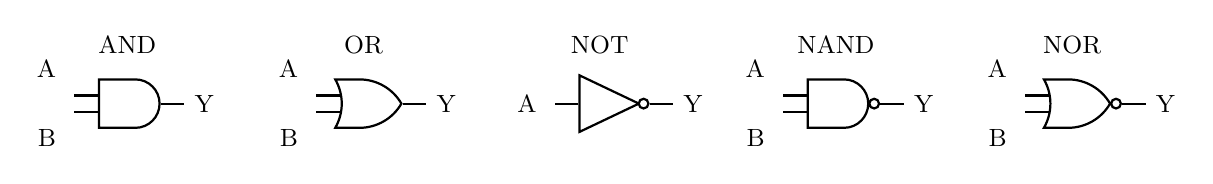
\begin{tikzpicture}[circuit logic US, thick, 
    every node/.style={font=\small}]
    
    % 与门 (AND)
    \node[and gate] at (0,0) (and) {};
    \draw (and.input 1) -- ++(-0.3,0) coordinate (a1);
    \draw (and.input 2) -- ++(-0.3,0) coordinate (a2);
    \draw (and.output) -- ++(0.3,0) node[right] {Y};
    \node[above left=0.1cm and 0.1cm] at (a1) {A};
    \node[below left=0.1cm and 0.1cm] at (a2) {B};
    \node[above=0.5cm] at (and.center) {AND};
    
    % 或门 (OR)
    \node[or gate] at (3,0) (or) {};
    \draw (or.input 1) -- ++(-0.3,0) coordinate (o1);
    \draw (or.input 2) -- ++(-0.3,0) coordinate (o2);
    \draw (or.output) -- ++(0.3,0) node[right] {Y};
    \node[above left=0.1cm and 0.1cm] at (o1) {A};
    \node[below left=0.1cm and 0.1cm] at (o2) {B};
    \node[above=0.5cm] at (or.center) {OR};
    
    % 非门 (NOT)
    \node[not gate] at (6,0) (not) {};
    \draw (not.input) -- ++(-0.3,0) coordinate (n1);
    \draw (not.output) -- ++(0.3,0) node[right] {Y};
    \node[left=0.1cm] at (n1) {A};
    \node[above=0.5cm] at (not.center) {NOT};
    
    % 与非门 (NAND)
    \node[nand gate] at (9,0) (nand) {};
    \draw (nand.input 1) -- ++(-0.3,0) coordinate (na1);
    \draw (nand.input 2) -- ++(-0.3,0) coordinate (na2);
    \draw (nand.output) -- ++(0.3,0) node[right] {Y};
    \node[above left=0.1cm and 0.1cm] at (na1) {A};
    \node[below left=0.1cm and 0.1cm] at (na2) {B};
    \node[above=0.5cm] at (nand.center) {NAND};
    
    % 或非门 (NOR)
    \node[nor gate] at (12,0) (nor) {};
    \draw (nor.input 1) -- ++(-0.3,0) coordinate (no1);
    \draw (nor.input 2) -- ++(-0.3,0) coordinate (no2);
    \draw (nor.output) -- ++(0.3,0) node[right] {Y};
    \node[above left=0.1cm and 0.1cm] at (no1) {A};
    \node[below left=0.1cm and 0.1cm] at (no2) {B};
    \node[above=0.5cm] at (nor.center) {NOR};
\end{tikzpicture}
\end{center}
\newpage
\section{命题演算的关系式}
$P\Leftrightarrow Q$（逻辑等价）的定义是：$P\leftrightarrow Q$为永真式/重言式；$P\Rightarrow Q$（逻辑蕴含）的定义是：$P\rightarrow Q$为永真式；

证明两个命题公式等价，方法是：1.比较真值表；2. 等价运算（使用等价符号$\Leftrightarrow$）

置换规则：它允许在逻辑公式中，用逻辑等价的子公式替换另一个子公式，而不改变原公式的真值。
\begin{definition}{对偶式}
    在命题逻辑中，设$A$是一个仅包含联结词$\neg$（否定）、$\land$（合取）和$\lor$（析取）的命题公式。$A$的\textbf{对偶式}是通过将$A$中所有的$\land$替换为$\lor$，所有的$\lor$替换为$\land$，同时将所有的$1$（真）替换为$0$（假），所有的$0$（假）替换为$1$（真）而得到的新公式，记作$A^*$
\end{definition}
\begin{theorem}{对偶式的性质}
设$A$和$B$是仅包含联结词$\neg$、$\land$和$\lor$的命题公式，$A^*$和$B^*$分别是它们的对偶式\\
1. \textbf{对偶原理}：若$A \Leftrightarrow B$，则$A^* \Leftrightarrow B^*$。逻辑等价关系在对偶变换下保持不变。\\
2. \textbf{对偶的对偶}：$A \Leftrightarrow (A^*)^*$，即$A$的对偶式的对偶式等于$A$本身。\\
3. \textbf{永真式与永假式的对偶}：若$A$永真，则$A^*$永假；若$A$永假，则$A^*$永真。\\
4. \textbf{对偶式的否定}：$\neg A \Leftrightarrow (\neg A^*)^*$，其中$\neg A^*$表示先将$A$中的原子命题取否定，再求对偶式。\\
5. \textbf{对偶式的运算}：$(A \land B)^* = A^* \lor B^*$，$(A \lor B)^* = A^* \land B^*$，$(\neg A)^* = \neg (A^*)$\\
6. $A\Rightarrow B$的充分必要条件是$B^* \Rightarrow A^*$
\end{theorem}
性质5是由定义导出的，性质4是因为否定运算在对偶变换下保持不变，对偶式定义只涉及交换$\land$和$\lor$，性质3更显然，因为永真式为1，永假式为0，对偶变换后显然颠倒。

下面证明性质6

\textbf{第一步：证明如果$A \Rightarrow B$，则$B^* \Rightarrow A^*$}，由于$A \Rightarrow B$，所以$A \rightarrow B$是永真式。根据对偶式的性质，永真式的对偶是永假式，因此$(A \rightarrow B)^* $是永假式，将蕴含式转换为基本联结词：$A \rightarrow B \Leftrightarrow \neg A \lor B$，所以$(\neg A \lor B)^* \text{是永假式}$，根据对偶式的定义：$(\neg A \lor B)^* = (\neg A)^* \land B^* = \neg A^* \land B^*$，因此$\neg A^* \land B^*$是永假式，这意味着对于所有赋值，$\neg A^* \land B^*$都为假。两边同时取否定得到$\neg A^* \rightarrow \neg B^*$为真，即$B^* \rightarrow A^*$为永真式，所以$B^* \Rightarrow A^*$。

\textbf{第二步：证明如果$B^* \Rightarrow A^*$，则$A \Rightarrow B$}由于$B^* \Rightarrow A^*$，根据第一步的结论（将$A$替换为$B^*$，$B$替换为$A^*$），我们有：$(A^*)^* \Rightarrow (B^*)^*$，根据对偶式的性质，$(A^*)^* = A$，$(B^*)^* = B$，所以$A \Rightarrow B$。综上，$A \Rightarrow B$当且仅当$B^* \Rightarrow A^*$。
\begin{theorem}{重要等价关系}
\noindent\textbf{1. 基本等价关系}\\
双重否定律：$\neg\neg P \Leftrightarrow P$\\
等幂律（幂等律）：$P \lor P \Leftrightarrow P$，$P \land P \Leftrightarrow P$\\
交换律：$P \lor Q \Leftrightarrow Q \lor P$，$P \land Q \Leftrightarrow Q \land P$\\
结合律：$(P \lor Q) \lor R \Leftrightarrow P \lor (Q \lor R)$，$(P \land Q) \land R \Leftrightarrow P \land (Q \land R)$\\
分配律：$P \lor (Q \land R) \Leftrightarrow (P \lor Q) \land (P \lor R)$，$P \land (Q \lor R) \Leftrightarrow (P \land Q) \lor (P \land R)$\\
吸收律：$P \lor (P \land Q) \Leftrightarrow P$，$P \land (P \lor Q) \Leftrightarrow P$\\
德摩根律：$\neg(P \lor Q) \Leftrightarrow \neg P \land \neg Q$，$\neg(P \land Q) \Leftrightarrow \neg P \lor \neg Q$\\
\noindent\textbf{2. 常元相关等价关系}\\
零元律：$P \lor 1 \Leftrightarrow 1$，$P \land 0 \Leftrightarrow 0$\quad 同一律：$P \lor 0 \Leftrightarrow P$，$P \land 1 \Leftrightarrow P$\\
排中律：$P \lor \neg P \Leftrightarrow 1$\quad 矛盾律：$P \land \neg P \Leftrightarrow 0$\\
\noindent\textbf{3. 蕴含与等价关系}\\
蕴含等值式：$P \rightarrow Q \Leftrightarrow \neg P \lor Q$（“$P$发生且$Q$不发生”是不可能的）\\
逆否等值式：$P \rightarrow Q \Leftrightarrow \neg Q \rightarrow \neg P$\\
等价等值式：$P \leftrightarrow Q \Leftrightarrow (P \rightarrow Q) \land (Q \rightarrow P)$\\
等价否定等值式：$P \leftrightarrow Q \Leftrightarrow \neg P \leftrightarrow \neg Q$\\
归谬论：$(P \rightarrow Q) \land (P \rightarrow \neg Q) \Leftrightarrow \neg P$（不可能同时蕴含正反面）\\
\noindent\textbf{4. 其他重要等价关系}\\
输出律：$(P \land Q) \rightarrow R \Leftrightarrow P \rightarrow (Q \rightarrow R)$
\end{theorem}
应该注意，形如$A\Leftrightarrow B,A\Rightarrow B$不是命题公式，而是命题关系式。而应用这些等价关系式可以证明公式互相等价，或者求主析取范式，主合取范式。解题过程中应该利用等价符号。

但是当题目要证明“若$p$则$q$”这样的蕴含关系，就可以出新的考题。我们可以将要证明的蕴含关系利用蕴含式写出来，再证明其永真（解题过程中应该利用等价符号），这就需要用到等价关系式（或者真值表）。

但是，当转化出来的命题公式的蕴含前件或者后件中含有较多的命题变元，就需要使用推理定律，并使用编号1234一步步写出推理过程，而不是这里的等价关系式，解题过程中也不应该出现等价符号。考试一般考“利用构造法验证推理是否有效”（指的是构造定理证明系统）。

上面提到的输出律，即\textbf{CP规则}:
\begin{theorem}{CP规则（附加前提规则）}
对于任意公式$A_1, A_2, \ldots, A_n, B, C$，如果$A_1, A_2, \ldots, A_n, B$可以推出$C$，则$A_1, A_2, \ldots, A_n$可以推出$B \rightarrow C$。

这意味着，如果我们能从前提集合和临时假设$B$推导出$C$，那么我们就能从原前提集合推导出条件语句$B \rightarrow C$，而不再依赖假设$B$。
\end{theorem}
除了这个规则外，还有若干规则需要遵循：\\
1. 前提引入规则：在证明的任何步骤中，可以随时引入已知的前提条件。在证明过程中，并不需要用完所有给定的前提。关键是选择能够有效推导出结论的前提组合。当前提自身存在矛盾时，并不影响这个规则的合理性，因为矛盾本身已经足以推出任何结论。\\
2. 结论引入规则：从已知条件出发，通过有效的推理规则推导出新的结论。\\
3. 置换规则：在证明过程中，可以用逻辑等价的公式替换原公式，而不改变推理的有效性。最后的置换规则恰恰给出了推理中“不允许使用等价符号”的替代方案。
\begin{theorem}{蕴含关系式}
\textbf{1. 化简律}：$P \land Q \Rightarrow P$（或$P \land Q \Rightarrow Q$），（抓住重点，忽略次要）\\
\textbf{2. 附加律}：$P \Rightarrow P \lor Q$ ，（有真则真，多说不妨）\\
\textbf{3. 假言推理（分离规则）}：$(P \rightarrow Q) \land P \Rightarrow Q$（有条件就执行） \\
\textbf{4. 拒取式}：$(P \rightarrow Q) \land \neg Q \Rightarrow \neg P$ （结果不成立，前提必为假）\\
\textbf{5. 假言三段论}：$(P \rightarrow Q) \land (Q \rightarrow R) \Rightarrow (P \rightarrow R)$ （环环相扣）\\
\textbf{6. 析取三段论}：$(P \lor Q) \land \neg P \Rightarrow Q$ （非此即彼）\\
\textbf{7. 构造性二难}：$[(P \rightarrow Q) \land (R \rightarrow S)\land(P \lor R)] \Rightarrow Q \lor S$ （分兵二路，两路夹击）\\
\textbf{8. 破坏性二难}：$[(P \rightarrow Q) \land (R \rightarrow S)\land(\neg Q \lor \neg S)] \Rightarrow \neg P \lor \neg R$ \\
\textbf{9. 等价三段论}：$(P \leftrightarrow Q) \land (Q \leftrightarrow R) \Rightarrow (P \leftrightarrow R)$ \\
\textbf{10. 归结式}：$(P \lor Q) \land (\neg P \lor R) \Rightarrow (Q \lor R)$（两头下注，必中一个）
\end{theorem}
归结证明是一种基于归结原理的自动定理证明方法，基础是“归结式”：对于两个子句$C_1 = P \lor A$和$C_2 = \neg P \lor B$，可以通过消去互补文字$P$和$\neg P$，得到归结式$A \lor B$。解题过程是：先将前提集合与结论的否定转化为合取范式，得到子句集合，然后通过反复应用归结规则推导新的子句；如果能够推导出空子句（矛盾），则说明前提集合与结论的否定不可同时满足，从而原结论由前提推出。

除了利用这些推理规则并使用演绎法进行推理，也可以先附加前提（CP），再直接证明。或者先附加结论的否定（归谬法）再进行间接推演。
\begin{definition}{相容}
    如果存在一个真值赋值使得所有公式$A_1, A_2, \ldots, A_n$同时为真，则称它们是\textbf{相容的}（一致的）；否则称它们是\textbf{不相容的}（矛盾的），即这些命题公式的合取式为矛盾式。
\end{definition}
有了这个思路，我们可以将结论取否定加入到前提条件集合中，证明前提集合与结论的否定不相容，从而证明原来的结论是正确的。
\section{析取范式，合取范式}
\begin{definition}{析取范式和合取范式，极小项极大项，主析取，主合取范式}
\textbf{析取范式}是若干个\textbf{简单合取式}（文字的合取）的析取，形如：$(P \land \neg Q) \lor (R \land S) \lor \cdots$\\
\textbf{合取范式}是若干个\textbf{简单析取式}（文字的析取）的合取，形如：$(P \lor \neg Q) \land (R \lor S) \land \cdots$\\
任何命题公式都存在等价的析取范式和合取范式，可通过蕴含等价、内移否定、分配律得。\\
\textbf{极小项}是包含所有命题变元或其否定的简单合取式，每个变元恰好出现一次。例如，对于变元$P,Q$，极小项有：$P \land Q$，$P \land \neg Q$，$\neg P \land Q$，$\neg P \land \neg Q$。\\
\textbf{极大项}是包含所有命题变元或其否定的简单析取式，每个变元恰好出现一次。例如，对于变元$P,Q$，极大项有：$P \lor Q$，$P \lor \neg Q$，$\neg P \lor Q$，$\neg P \lor \neg Q$。\\
\textbf{主析取范式}是由极小项组成的析取范式，每个极小项对应公式的一个成真赋值。\\
\textbf{主合取范式}是由极大项组成的合取范式，每个极大项对应公式的一个成假赋值。\\
任何命题公式都存在等价的唯一主析取范式和主合取范式。永真式的主合取范式为空（无极大项），永假式的主析取范式为空（无极小项）。
\end{definition}
所以由上述定义得知，主析取范式或主合取范式中不一定有极小项或者极大项。极小项一般用小写$m_i$表示，极大项一般用大写$M_i$表示。

关于成真赋值和成假赋值与谁对应，这里提供理解和记忆的方式：

由于析取范式由若干个简单合取式（极小项）通过析取联结词连接而成，而析取运算具有"一真即真"的特性，这类似于逻辑代数中的"或"运算：$0$（假）参与运算不改变结果（相当于没有贡献），而每个$1$（真）项（对应极小项为真）都会使结果为真。因此，为了和原命题保持等价关系，主析取范式的每一个极小项都要对应着公式的一个成真赋值，不然就不可以代表（或者等价于）原命题公式。

进而，将真值表中每个成真赋值对应的二进制数转化为十进制，即可得到该极小项的下标（如赋值$P=1, Q=0, R=1$对应$m_5$）。主析取范式就是所有这些极小项（如$m_2, m_5, m_7$）用逻辑加连接起来的形式：$\sum(2,5,7)$。

由于合取范式由若干个简单析取式（极大项）通过合取联结词连接而成，而合取运算具有"一假即假"的特性，这类似于逻辑代数中的"与"运算：$1$（真）参与运算不改变结果（相当于没有贡献），而每个$0$（假）项（对应极大项为假）都会使结果为假。因此，为了和原命题保持等价关系，主合取范式的每一个极大项都要对应着公式的一个成假赋值，不然就不可以代表（或者等价于）原命题公式。

进而，将真值表中每个成假赋值对应的二进制数转化为十进制，即可得到该极大项的下标（如赋值$P=1, Q=0, R=1$对应$M_5$）。主合取范式就是所有这些极大项（如$M_2, M_5, M_7$）用逻辑乘连接起来的形式$\prod(2,5,7)$

对主析取范式（主合取范式）使用分配律（可以理解为多项式乘法）可以得到等价的主合取范式（主析取范式）。
\[(P \land Q) \lor (\neg P \land \neg Q) = (P\lor \neg P)\land (P\lor \neg Q)\land (Q\lor \neg P)\land (Q\lor \neg Q)= (P\lor \neg Q)\land (Q\lor \neg P) \]
\begin{example}[2023年真题]
    用等值演算法求取下列公式：$(\neg P\to Q)\to(P\lor\neg Q)$的合取范式
\end{example}
\vspace{-30pt}
\begin{align*}
 (\neg P \to Q) \to (P \lor \neg Q) 
\Leftrightarrow &  \neg (P \lor Q) \lor (P \lor \neg Q) \quad \text{（蕴含等值式）} \\
\Leftrightarrow & (\neg P \land \neg Q) \lor (P \lor \neg Q) \quad \text{（德摩根定律）} \\
\Leftrightarrow & [\neg P \lor (P \lor \neg Q)] \land [\neg Q \lor (P \lor \neg Q)] \quad \text{（分配律）} \\
\Leftrightarrow & [(\neg P \lor P) \lor \neg Q] \land [P \lor (\neg Q \lor \neg Q)] \quad \text{（结合律）} \\
\Leftrightarrow & P \lor \neg Q 
\end{align*}
\begin{example}[2023年真题]
构造下面推理的证明。前提：$p\lor q, p\to \neg r, s\to t,\neg s\to r, \neg t$，结论：$q$
\end{example}
\vspace{-30pt}
\begin{align*}
1\quad& s\to t&\text{前提引入}\\
2\quad& \neg s\lor t&\text{蕴含等值式（从1）}\\
3\quad& \neg t&\text{前提引入}\\
4\quad& \neg s&\text{析取三段论（从2,3）}\\
5\quad& \neg s\to r&\text{前提引入}\\
6\quad& r&\text{假言推理（从4,5）}\\
7\quad& p\to \neg r&\text{前提引入}\\
8\quad& \neg p&\text{拒取式（从6,7）}\\
9\quad& p\lor q&\text{前提引入}\\
10\quad& q&\text{析取三段论（从8,9）}
\end{align*}
\begin{example}
    下面哪些是合取范式？\\
    A. $q$\quad B. $p\lor q$\quad C. $(p\lor q)\land(\neg p\lor q)$\\
    下面哪些是同时是析取范式和合取范式？\\
    A. $p\lor q$\quad B. $q$\quad C. $p\land \neg q$
\end{example}
答案：都是ABC


% ===== Copied from learn-lisanshuxue/chapters/chap2.tex =====
\chapter{谓词逻辑}
\section{谓词逻辑基本概念}
\begin{definition}{个体词~谓词~n元谓词~个体常元变元~谓词常项变项}
在谓词逻辑中，命题被分解为个体词和谓词两部分。\\
个体词是命题中表示具体或抽象对象的词，包括表示特定个体的个体常元（如$a, b, c$）和表示不确定个体的个体变元（如$x, y, z$）。\\
谓词是用来说明个体性质或个体间关系的词，包括表示特定性质或关系的谓词常项（如$P, Q, R$）和表示不确定性质或关系的谓词变项（如$F, G, H$）。n元谓词是涉及$n$个个体的谓词，表示$n$元关系，如一元谓词$P(x)$描述个体性质，二元谓词$R(x,y)$描述两个体间关系，n元谓词$F(x_1,x_2,\ldots,x_n)$描述n个个体的关系。
\end{definition}
\begin{definition}{谓词表达式，命题函数，个体域，论述域}
在谓词逻辑中，谓词表达式是由谓词和个体词组成的符号串，用于表示个体的性质或个体间的关系，例如$P(x)$、$R(a, b)$等。\\
命题函数是以个体变元（其取值范围就是个体域，也称作论述域）为自变量的函数，其取值是一个命题，当个体变元被特定个体常元替换时，命题函数转化为一个具体的命题。例如，$P(x)$是一个命题函数，当$x$取值为$a$时，$P(a)$成为一个命题。命题函数的真值取决于个体变元的取值和谓词的含义。
\end{definition}
可以看出，闭式谓词公式在给定解释下可以判断真值；含自由变元的命题函数需要给自由变元赋值后才有真值。个体域可以是无限或者有限的，没有特别说明时，个体变元的论述域指的是把整个宇宙中一切事物都作为对象的集合，所以当大题没有说个体域是什么时，最好不要想当然的自我设想个体域，比如说有的题目说“所以人都是学生”，那么最好还是设置命题函数“$M(x):x$是人”，或者声明个体域$x$是人，不要直接不管了。
\begin{definition}{量词}
量词是用于表示个体变元在个体域中取值范围的逻辑符号。\\
\textbf{全称量词}（$\forall$）：表示"对所有"或"任意"，如$\forall x P(x)$表示"对所有$x$，$P(x)$成立"。\\
\textbf{存在量词}（$\exists$）：表示"存在"或"至少有一个"，如$\exists x P(x)$表示"存在$x$使得$P(x)$成立"。\\
除了这两种基本量词外，还有一些扩展的量词表示法：\\
\textbf{唯一存在量词}（$\exists!$）：表示"存在唯一的"，如$\exists! x P(x)$表示"存在唯一的$x$使得$P(x)$成立"\\
\textbf{计数量词}：如$\exists_n x P(x)$表示"恰好有$n$个$x$满足$P(x)$"
\end{definition}
注意，在使用全称量词时，表示个体范围的特性谓词和表示个体性质的谓词构成条件关系式：$\forall x (P(x) \rightarrow Q(x))$；使用存在量词时，表示个体范围的特性谓词和表示个体性质的谓词构成合取关系式：$\exists x (P(x) \land Q(x))$。

考虑命题"所有大学生都年轻"。如果我们错误地用合取式：$\forall x (Student(x) \land Young(x))$这表示"每个个体都是大学生并且年轻"——要求宇宙中\textbf{所有个体}都必须是大学生！这显然过强了。正确的条件式：$\forall x (Student(x) \rightarrow Young(x))$只对"是大学生"的那些个体施加"年轻"的要求，对非大学生个体没有要求，这才是符合题意的。

考虑命题"有大学生聪明"。如果我们错误地用条件式：$\exists x (Student(x) \rightarrow Smart(x))$这个公式在逻辑上等价于$\exists x (\neg Student(x) \lor Smart(x))$，只要存在\textbf{任意一个非大学生}，这个公式就为真，完全偏离原意。而$\exists x (Student(x) \land Smart(x))$表达了"存在一个个体既是大学生又聪明"的含义。

实际上，两种表达在特定条件下可以转换：$\forall x (P(x) \rightarrow Q(x)) \Leftrightarrow \neg \exists x (P(x) \land \neg Q(x))$
\begin{definition}{谓词演算的合式公式，简称谓词合式公式}
合式公式是谓词逻辑中形式推理和语义解释的基本单位，其递归定义如下：\\
1. 原子公式是合式公式：如果$P$是$n$元谓词，$t_1, t_2, \ldots, t_n$是项（个体常元、个体变元或函数），则$P(t_1, t_2, \ldots, t_n)$是合式公式\\
2. 逻辑联结词组合：如果$A$和$B$是合式公式，则$(\neg A)$、$(A \land B)$、$(A \lor B)$、$(A \rightarrow B)$、$(A \leftrightarrow B)$也是合式公式\\
3. 量词组合：如果$A$是合式公式，$x$是个体变元，则$(\forall x A)$和$(\exists x A)$也是合式公式\\
4. 只有有限次应用上述规则构成的表达式才是合式公式
\end{definition}
\begin{definition}{指导变元，辖域，约束变元，约束出现，自由变元，自由出现，闭式}
在谓词逻辑中，量词和变元的使用涉及以下重要概念：\\
\textbf{指导变元}：紧跟在量词后面的个体变元称为指导变元，如$\forall x$中的$x$和$\exists y$中的$y$。\\
\textbf{辖域}：量词所作用的公式范围称为该量词的辖域。如$\forall x (P(x) \rightarrow Q(x))$中，$(P(x) \rightarrow Q(x))$是$\forall x$的辖域。\\
\textbf{约束变元}：在量词辖域内出现且与该量词指导变元相同的个体变元称为约束变元。\\
\textbf{约束出现}：个体变元在公式中的某次出现如果处于某个量词的辖域内，且与该量词的指导变元相同，则称为约束出现。\\
\textbf{自由变元}：在公式中不被任何量词约束的个体变元称为自由变元。\\
\textbf{自由出现}：个体变元在公式中的某次出现如果不是约束出现，则称为自由出现。\\
\textbf{闭式}：不包含任何自由出现的个体变元的谓词公式称为闭式。闭式中所有个体变元都是约束出现的，这样的公式具有确定的真值。
\end{definition}
例如，在公式$\forall x (P(x,y) \rightarrow \exists z Q(x,z))$中：$x$和$z$是指导变元，$(P(x,y) \rightarrow \exists z Q(x,z))$是$\forall x$的辖域，$Q(x,z)$是$\exists z$的辖域，第一个$x$和第二个$x$是约束出现（被$\forall x$约束），$y$是自由出现（自由变元），$z$是约束出现（被$\exists z$约束），该公式不是闭式，因为包含自由变元$y$。

\begin{definition}{谓词公式的解释和分类}
谓词公式的解释是指为公式中的符号赋予具体含义的过程，包括以下四个组成部分：\\
1. \textbf{个体域} $D$：一个非空集合，规定个体变元的取值范围\\
2. \textbf{个体常元的指定}：为每个个体常元指定$D$中的一个特定元素\\
3. \textbf{函数符号的指定}：为每个$n$元函数符号指定$D^n$到$D$的映射\\
4. \textbf{谓词符号的指定}：为每个$n$元谓词符号指定$D^n$到$\{\text{真,假}\}$的映射\\
给定解释$I$和公式$A$，可以通过递归方式计算$A$在$I$下的真值。闭式在给定解释下有确定真值，但在不同解释下真值可能不同；包含自由变元的公式真值还取决于自由变元的取值。公式$A$是永真式当且仅当$A$在所有解释下为真；$A$是可满足式当且仅当存在解释使$A$为真；$A$是永假式当且仅当$A$在所有解释下为假。
\end{definition}
谓词公式判断类型是比较困难的，为了判断一些简单的情形，可以定义代换实例：
\begin{definition}{命题公式的谓词代换实例}
命题公式的谓词代换实例，是指通过将命题逻辑中的命题公式中的命题变元替换为谓词公式而得到的谓词公式。具体来说，设$A$是一个命题公式，其中包含命题变元$P_1, P_2, \ldots, P_n$。如果用一个谓词公式$B_i$（$i = 1, 2, \ldots, n$）替换$A$中的每个命题变元$P_i$，则得到的新公式$A'$称为$A$的一个代换实例。\\
代换实例保持了原命题公式的逻辑结构，只是将原子命题替换为谓词公式。如果原命题公式是永真式（矛盾式），则其所有代换实例也是永真式（矛盾式）。
\end{definition}
例如，命题公式 $P \rightarrow (Q \land P)$ 的一个代换实例可以是
\[
\forall x\, P(x) \rightarrow (\exists y\, Q(y) \land \forall x\, P(x)).
\]
从代换实例的视角来看，有些谓词公式也可以像命题公式那样做等价变换，从而证明公式之间的等价关系或蕴含关系。这时就需要用到前面介绍的推理定律，详见第 2.3 节。
\section{换名，前束范式}
换名的动机是让谓词公式中尽量不要出现同样的变元，避免变量名的混淆，同时便于进行逻辑推理。

约束变元换名规则允许在公式中更改约束变元的名称，而不改变公式的逻辑含义。例如，将公式 $\forall x (P(x) \rightarrow \exists y\, Q(x,y))$ 中受约束的变元 $x$ 换为 $z$，可得到等价公式 $\forall z (P(z) \rightarrow \exists y\, Q(z,y))$。换名时需要满足以下要求：
\begin{enumerate}
    \item 只能更改约束变元的名称，不能更改自由变元。
    \item 换名必须在整个量词的辖域内一致进行。
    \item 新变元名称不能与公式中已有的自由变元同名。
    \item 多个量词约束的同名变元可以按各自的辖域分别换名，但每次换名都必须只在对应量词的辖域内一致进行。
\end{enumerate}

自由变元代入规则允许用项替换公式中的自由变元。例如将 $\forall x P(x,y)$ 中的自由变元 $y$ 用常元 $a$ 代入，得到 $\forall x P(x,a)$，要求如下：\\
1. 代入必须对自由变元的所有自由出现同时进行\\
2. 代入项中不能含有在公式中受约束的变元\\
3. 代入项必须对该自由变元可代入，避免代入后被原有量词捕获

注意，约束变元换名改变的是变元符号，不改变变元的性质（仍是约束变元），并保持公式的逻辑等价性；自由变元代入是用具体的项（常元、函数或其他变元）替换自由变元，得到的是原公式的一个代换实例，一般不与原来的含自由变元公式逻辑等价。

举一个例子，比如谓词公式：$\forall x (P(x,y) \rightarrow \exists y Q(x,y))$，这个公式存在两个问题：一是自由变元$y$与约束变元$y$同名，容易引起混淆，二是量词$\forall x$和$\exists y$的约束变元$x$和$y$在公式中混合使用，不利于逻辑推理。下面换名：

\textbf{第一步：自由变元代入}：将自由变元$y$用常元$a$代入：$\forall x (P(x,a) \rightarrow \exists y Q(x,y))$

\textbf{第二步：约束变元换名}：将存在量词$\exists y$的约束变元$y$换名为$z$：$\forall x (P(x,a) \rightarrow \exists z Q(x,z))$。经过两个规则的应用，我们得到的新公式：自由变元$y$已被具体化为常元$a$，约束变元$y$被换名为$z$，避免了名称冲突，现在公式中每个变元的角色清晰：$x$是$\forall$的约束变元，$z$是$\exists$的约束变元，$a$是常元。这里换名保持等价，而自由变元代入得到的是代换实例。

常常利用换名将谓词公式化为与其自身等价的规范形式，成为前束范式：
\begin{definition}{前束范式，首标，母式}
前束范式是谓词逻辑中的一种标准形式，其中所有量词都出现在公式的最前端，且其辖域延伸到公式的末尾。形式化地，一个公式是前束范式当且仅当它具有以下形式：\vspace{-10pt}
$$Q_1x_1Q_2x_2\cdots Q_nx_nM,\text{其中}Q_1x_1Q_2x_2\cdots Q_nx_n\text{为首标},M\text{为不含量词的母式}\vspace{-10pt}$$
其中：$Q_i$ ($i=1,2,\ldots,n$) 是量词符号（$\forall$ 或 $\exists$），$x_i$ ($i=1,2,\ldots,n$) 是个体变元。
\end{definition}
将任意谓词公式化为前束范式的步骤通常包括：消去蕴含联结词 $\rightarrow$ 和等价联结词 $\leftrightarrow$，将否定符号 $\neg$ 内移，使其只作用于原子公式，将量词向左移动，并适当换名避免变元冲突。

例如谓词公式$\forall x\forall y(\exists z(P(x,z)\land P(y,z))\to\exists uQ(x,y,u))$化为前束范式的过程是：
\begin{align*}
&\forall x\forall y(\exists z(P(x,z)\land P(y,z))\to\exists uQ(x,y,u))\\
&\Leftrightarrow \forall x\forall y(\neg\exists z(P(x,z)\land P(y,z))\lor\exists uQ(x,y,u))&\text{置换规则}\\
&\Leftrightarrow \forall x\forall y(\forall z(\neg P(x,z)\lor\neg P(y,z))\lor\exists uQ(x,y,u))&\text{置换规则}\\
&\Leftrightarrow \forall x\forall y\forall z\exists u(\neg P(x,z)\lor\neg P(y,z)\lor Q(x,y,u))&\text{量词辖域扩张}
\end{align*}
由于上面的$x,y$的辖域覆盖到公式末尾，而且$z$和$u$的虽然辖域不同，但名称不同，无需换名，下面再看一个需要换名的例子。
求下列谓词公式的前束范式：$\neg\exists xA(x)\to\forall yB(x,y)$
\begin{align*}
    &\neg\exists xA(x)\to\forall yB(x,y)\\
    &\Leftrightarrow \forall x\neg A(x)\to\forall yB(x,y)&\text{否定等价转换}\\
    &\Leftrightarrow \forall z\neg A(z)\to\forall yB(x,y)&\text{换名}\\
    &\Leftrightarrow \exists z\forall y(\neg A(z)\to B(x,y))&\text{量词辖域扩张}\\
    &\Leftrightarrow \exists z\forall y(A(z)\lor B(x,y))&\text{置换规则}
\end{align*}
\section{谓词公式的等价和蕴含关系式}
与上一章类似，当两个谓词公式$A$和$B$满足$A\leftrightarrow B$为永真式时，我们说$A$和$B$是等价的，等价关系式的形式为：$A\Leftrightarrow B$；当两个谓词公式$A$和$B$满足$A\rightarrow B$为永真式时，我们说$A$蕴含$B$，蕴含关系式的形式为：$A\Rightarrow B$。以下公式按通常一阶逻辑约定，个体域非空。
\begin{theorem}{常见的等价关系式}
1. 去括号：$\exists x(A(x)\to B(x))\Leftrightarrow \forall xA(x)\to \exists xB(x)$\\
2. 去括号（$B(x)$中的$x$为自由变元）：$\forall y(A(y)\to B(x))\Leftrightarrow \exists yA(y)\to B(x)$\\
3. 量词辖域扩张与收缩（$B$中不含$x$自由出现）：\\
$\forall x(A(x)\land B)\Leftrightarrow \forall xA(x)\land B,\quad \exists x(A(x)\land B)\Leftrightarrow \exists xA(x)\land B$\\
$\forall x(A(x)\lor B)\Leftrightarrow \forall xA(x)\lor B,\quad \exists x(A(x)\lor B)\Leftrightarrow \exists xA(x)\lor B$\\
4. 去括号（$B$不含$x$）：$\forall x(A(x)\to B)\Leftrightarrow \exists xA(x)\to B\quad  \exists x(A(x)\to B)\Leftrightarrow \forall xA(x)\to B$\\
5. 分配律：$\forall x(A(x)\land B(x))\Leftrightarrow \forall xA(x)\land \forall xB(x)\quad \exists x(A(x)\lor B(x))\Leftrightarrow \exists xA(x)\lor \exists xB(x)$\\
6. 交换律：$\forall x\forall y A(x,y)\Leftrightarrow \forall y\forall x A(x,y)\quad \exists x\exists y A(x,y)\Leftrightarrow \exists y\exists x A(x,y)$
\end{theorem}
3和4即书上给出的量词辖域扩张与收缩律，使用时要注意被移出量词辖域的公式中不能含有该量词变量的自由出现。上面的公式利用等价变形都可以解决。

1. 左边说“至少有一个$x$，能够确保：如果它满足$A$，那么它也满足$B$”。右边说“如果所有的$x$都满足$A$，那么至少有一个$x$满足$B$”。例如：“假设你是老师，你承诺说你会找一些幸运儿学生，如果他们来上课就能及格”，这等价于“如果所有学生都来上课，那么有学生能及格”，因为你总要挑选学生给到及格。

2. 需要注意在这个公式中，$B(x)$中的变元是自由变元（没有被任何量词约束），因此两边都表示关于某个特定个体$x$的陈述。左边说"对任何一个$y$，如果$y$具有性质$A$，那么$x$具有性质$B$"；右边说"如果存在某个个体具有性质$A$，那么$x$具有性质$B$"。例如，"如果任何人都是医生，那么张三健康"等价于"如果有医生存在，那么张三健康"。由于$x$是自由变元，两边讨论的都是同一个特定的$x$（这里也可以视作存在量词引入），$B(x)$描述的是这个特定个体的性质，不受量词影响。

3. 当B是与x无关的事实陈述时，可以把B从量词中“提出来”。例如，“对所有学生，今天下雨且他们要考试”等价于“今天下雨且所有学生都要考试”。

4. 左边说“对每个个体，如果它满足$A$，就导致同一个与$x$无关的结论$B$”；右边说“只要存在满足$A$的个体，就导致$B$”。例如，“每个学生若作弊就取消考试”等价于“只要有学生作弊就取消考试”。

5. “每个人都既聪明又勤奋”等价于“每个人都聪明且每个人都勤奋”。“有人会唱歌或跳舞”等价于“有人会唱歌或者有人会跳舞”。

6. “任何两个人都是朋友”等价于“对任何人来说，与任何人都是朋友”，量词顺序不影响含义。“存在两个人是朋友”等价于“存在这样两个人，他们是朋友”，存在量词顺序也不影响含义。
\begin{example}
    0元谓词公式是命题吗？
\end{example}
是。
\begin{theorem}{常见的蕴含关系式（结论的弱化，也可以理解为前提的增多）}
1. $\exists xA(x)\to\exists xB(x)\Rightarrow\exists x(A(x)\to B(x))$\\
2. $\forall xA(x)\to \exists xB(x)\Rightarrow \exists x(A(x)\to B(x))$\\
3. $\forall xA(x)\lor \forall xB(x)\Rightarrow \forall x(A(x)\lor B(x))$\\
3'. $\forall x(A(x)\lor B(x))\Rightarrow \neg\forall xA(x)\to\exists xB(x)$\\
3''. $\forall x(A(x)\lor B(x))\Rightarrow \forall xA(x)\lor \exists xB(x)$\\
4. $\exists x(A(x)\land B(x))\Rightarrow \exists xA(x)\land \exists xB(x)$\\
5. $\forall x(A(x)\to B(x))\Rightarrow \forall xA(x)\to \forall xB(x)$\\
6. $\forall x\forall yA(x,y)\Rightarrow \forall xA(x,x)$\\
7. $\exists xA(x,x)\Rightarrow \exists x\exists yA(x,y)$\\
8. $\forall x\forall yA(x,y)\Rightarrow \exists y\forall xA(x,y)\Rightarrow \forall x\exists yA(x,y)\Rightarrow \exists x\exists yA(x,y)$
\end{theorem}
1. 如果存在某个$x$满足$A(x)$，那么存在某个$x$满足$B(x)$。注意，这里的两个$x$可能不是同一个个体，也可能是同一个个体，当为后一种情况，就得到了蕴含后件。所以蕴含关系 $\exists xA(x)\to\exists xB(x)\Rightarrow\exists x(A(x)\to B(x))$ 成立。

2. 如果所有$x$满足$A(x)$，那么存在某个$x$满足$B(x)$。单独考虑这个对$B(x)$量身定制的$x$也会满足$A(x)$，此时$A(x)\to B(x)$成立，蕴含关系 $\forall xA(x)\to \exists xB(x)\Rightarrow \exists x(A(x)\to B(x))$ 成立。

3. 左边是一个强条件：要么所有个体都满足$A$，要么所有个体都满足$B$。右边是一个弱条件：每个个体至少满足$A$或$B$之一。显然，如果左边成立，那么右边必须成立，因为如果所有个体都满足$A$，那么每个个体都满足$A$，所以满足$A$或$B$；类似如果所有个体都满足$B$，也一样。但反过来不一定成立：可能有些个体满足$A$但不满足$B$，有些满足$B$但不满足$A$，所以右边真但左边假，因此蕴含关系 $\forall xA(x)\lor \forall xB(x)\Rightarrow \forall x(A(x)\lor B(x))$ 成立。而另一个蕴含关系式作为例题安排在后面了。

4. 如果存在一个个体同时满足$A$和$B$，那么当然存在满足$A$的个体（就是这个个体）和存在满足$B$的个体（也是这个个体），但是右边的两个$x$可能一样也可能不一样，蕴含关系 $\exists x(A(x)\land B(x))\Rightarrow \exists xA(x)\land \exists xB(x)$ 显然成立。

5. 每一个满足$A$的$x$都同时满足$B$，所以如果进一步知道所有$x$都满足$A$，就能推出所有$x$都满足$B$。注意，前提$\forall x(A(x)\to B(x))$不允许存在满足$A$但不满足$B$的个体。蕴含关系 $\forall x(A(x)\to B(x))\Rightarrow \forall xA(x)\to \forall xB(x)$ 显然成立。

6. 左边说$A$关系对所有个体对都成立。右边说$A$关系对所有自对（即个体与自身）都成立。如果左边成立，特别地，当$y=x$时，$A(x,x)$成立，因此蕴含关系 $\forall x\forall yA(x,y)\Rightarrow \forall xA(x,x)$ 成立。

7. 如果存在一个个体与自身满足$A$，那么取个体$x$和$y$（取$y=x$）满足$A$。所以左边蕴含右边，即 $\exists xA(x,x)\Rightarrow \exists x\exists yA(x,y)$ 。但可能$A(x,y)$成立对于$x$和$y$不同，$A(x,x)$不成立。

8. 从“全局$A$”到“存在万能$y$”（万能钥匙）到“每个$x$有对应$y$”（专用钥匙）到“存在一对”（碰运气），强度递减，蕴含关系成立。

上面的叙述其实已经用到了四大谓词逻辑推理规则：
\begin{theorem}{四大谓词逻辑推理规则}
1. 全称实例化 (Universal Instantiation, UI):从全称命题推出特定实例。\vspace{-10pt}
$$\forall x P(x) \Rightarrow P(c),\text{其中}c\text{是个体域中的任意个体}\vspace{-10pt}$$
使用要求与注意事项：$c$必须属于个体域中的个体，且$c$不能在$A(x)$中约束出现，可以对同一个全称命题进行多次实例化，得到不同的实例，实例化时保持变元的一致性。例如，从“所有人都会死”推出“苏格拉底会死”。\\
2. 存在实例化 (Existential Instantiation, EI)从存在命题推出特定实例。\vspace{-10pt}
$$\exists x P(x) \Rightarrow P(c),\text{其中}c\text{是个体域中的某个特定个体}\vspace{-10pt}$$
使用要求与注意事项：$c$必须是新引入的常元，不能和公式或推理证明过程中已有的常元或变元相同；若当前证明还有未解除的假设，$c$也不能出现在这些假设或最终结论中。EI允许公式中带有其他自由变元，它们可理解为参数，但新常元条件必须满足。例如，从"有人迟到了"推出"令$c$是某个迟到的人"\\
3. 全称泛化 (Universal Generalization, UG)从特定实例推出全称命题。\vspace{-10pt}
$$P(c) \Rightarrow \forall x P(x),\text{其中}c\text{是个体域中的任意个体}\vspace{-10pt}$$
使用要求与注意事项：这里的$c$必须代表任意对象，不能依赖特殊假设，也不能是由EI引入的特定常元；只有当证明没有用到$c$的特殊性质时，才能推广为全称命题。示例：通过证明任意一个三角形的内角和为180度，推出所有三角形的内角和为180度。\\
4. 存在泛化 (Existential Generalization, EG)：从特定实例推出存在命题。\vspace{-10pt}
$$P(c) \Rightarrow \exists x P(x),\text{其中}c\text{是个体域中的某个特定个体}\vspace{-10pt}$$
使用要求与注意事项：$c$可以是任意已知个体，但用$x$替换$c$形成$P(x)$时要避免变量捕获，也就是$x$不能被原公式中已有的量词错误绑定。示例：从“苏格拉底是哲学家”推出“存在哲学家”。\\
5. \textbf{易错点：在使用EI引入新常元后，不能再对该常元使用UG}
\end{theorem}
\noindent
\textbf{证明 1:} $\exists xA(x)\to\exists xB(x)\Rightarrow\exists x(A(x)\to B(x))$
\vspace{-10pt}
\begin{align*}
&(1)\ \exists xA(x) \to \exists xB(x) && \text{前提} \\
&(2)\ \neg\exists x(A(x)\to B(x)) && \text{临时假设（用于反证）} \\
&(3)\ \forall x\neg(A(x)\to B(x)) && \text{由(2)量词否定} \\
&(4)\ \forall x(A(x) \land \neg B(x)) && \text{由(3)蕴含等值式} \\
&(5)\ A(c) \land \neg B(c) && \text{由(4)UI，$c$任意} \\
&(6)\ A(c) && \text{由(5)化简} \\
&(7)\ \exists xA(x) && \text{由(6)EG} \\
&(8)\ \exists xB(x) && \text{由(1)(7)MP} \\
&(9)\ B(d) && \text{由(8)EI，$d$为新常量} \\
&(10)\ \neg B(d) && \text{由(4)UI（$x=d$）得$A(d) \land \neg B(d)$，化简} \\
&(11)\ B(d) \land \neg B(d) && \text{由(9)(10)合取} \\
&(12)\ \exists x(A(x)\to B(x)) && \text{由(2)(11)反证法}
\end{align*}

\noindent
\textbf{证明 2:} $\forall xA(x)\to \exists xB(x)\Rightarrow \exists x(A(x)\to B(x))$。这里按经典逻辑，对$\forall xA(x)$是否成立分类讨论。
\vspace{-10pt}
\begin{align*}
&(1)\ \forall xA(x) \to \exists xB(x) && \text{前提} \\
&(2)\ \text{假设 } \forall xA(x) && \text{情况1假设} \\
&(3)\ \exists xB(x) && \text{由(1)(2)MP} \\
&(4)\ B(c) && \text{由(3)EI，$c$为新常量} \\
&(5)\ A(c) && \text{由(2)UI} \\
&(6)\ A(c) \to B(c) && \text{由(4)条件引入} \\
&(7)\ \exists x(A(x)\to B(x)) && \text{由(6)EG} \\
&(8)\ \neg\forall xA(x) && \text{情况2假设} \\
&(9)\ \exists x\neg A(x) && \text{由(8)量词否定} \\
&(10)\ \neg A(d) && \text{由(9)EI，$d$为新常量} \\
&(11)\ A(d) \to B(d) && \text{由(10)（前件假则蕴含真）} \\
&(12)\ \exists x(A(x)\to B(x)) && \text{由(11)EG} \\
&(13)\ \exists x(A(x)\to B(x)) && \text{由(2)-(7)和(8)-(12)两种情况}
\end{align*}

\noindent
\textbf{证明 3.1:} $\forall xA(x)\lor \forall xB(x)\Rightarrow \forall x(A(x)\lor B(x))$
\vspace{-10pt}
\begin{align*}
&(1)\ \forall xA(x) \lor \forall xB(x) && \text{前提} \\
&(2)\ \text{设任意个体 $c$} && \text{UG的准备} \\
&(3)\ \text{假设 } \forall xA(x) && \text{情况1假设} \\
&(4)\ A(c) && \text{由(3)UI} \\
&(5)\ A(c) \lor B(c) && \text{由(4)添加析取} \\
&(6)\ \text{假设 } \forall xB(x) && \text{情况2假设} \\
&(7)\ B(c) && \text{由(6)UI} \\
&(8)\ A(c) \lor B(c) && \text{由(7)添加析取} \\
&(9)\ A(c) \lor B(c) && \text{由(1)(3)-(5)(6)-(8)析取消除} \\
&(10)\ \forall x(A(x)\lor B(x)) && \text{由(2)(9)UG}
\end{align*}

\noindent
\textbf{证明 3.2:} $\forall x(A(x)\lor B(x))\Rightarrow \neg\forall xA(x)\to\exists xB(x)$
\vspace{-10pt}
\begin{align*}
&(1)\ \forall x(A(x)\lor B(x)) && \text{前提} \\
&(2)\ \neg\forall xA(x) && \text{附加前提} \\
&(3)\ \exists x\neg A(x) && \text{由(2)量词否定} \\
&(4)\ \neg A(c) && \text{由(3)EI，$c$为新常量} \\
&(5)\ A(c) \lor B(c) && \text{由(1)UI} \\
&(6)\ B(c) && \text{由(4)(5)DS} \\
&(7)\ \exists xB(x) && \text{由(6)EG} \\
&(8)\ \neg\forall xA(x) \to \exists xB(x) && \text{由(2)(7)CP}
\end{align*}

\noindent
\textbf{证明 3.3:} $\forall x(A(x)\lor B(x))\Rightarrow \forall xA(x)\lor \exists xB(x)$
\vspace{-10pt}
\begin{align*}
&(1)\ \forall x(A(x)\lor B(x)) && \text{前提} \\
&(2)\ \neg(\forall xA(x) \lor \exists xB(x)) && \text{临时假设（反证）} \\
&(3)\ \neg\forall xA(x) \land \neg\exists xB(x) && \text{由(2)德摩根} \\
&(4)\ \neg\forall xA(x) && \text{由(3)化简} \\
&(5)\ \neg\exists xB(x) && \text{由(3)化简} \\
&(6)\ \forall x\neg B(x) && \text{由(5)量词否定} \\
&(7)\ \exists x\neg A(x) && \text{由(4)量词否定} \\
&(8)\ \neg A(c) && \text{由(7)EI，$c$为新常量} \\
&(9)\ A(c) \lor B(c) && \text{由(1)UI} \\
&(10)\ B(c) && \text{由(8)(9)DS} \\
&(11)\ \neg B(c) && \text{由(6)UI} \\
&(12)\ B(c) \land \neg B(c) && \text{由(10)(11)合取} \\
&(13)\ \forall xA(x) \lor \exists xB(x) && \text{由(2)(12)反证法}
\end{align*}

\noindent
\textbf{证明 4:} $\exists x(A(x)\land B(x))\Rightarrow \exists xA(x)\land \exists xB(x)$
\vspace{-10pt}
\begin{align*}
&(1)\ \exists x(A(x)\land B(x)) && \text{前提} \\
&(2)\ A(c) \land B(c) && \text{由(1)EI，$c$为新常量} \\
&(3)\ A(c) && \text{由(2)化简} \\
&(4)\ \exists xA(x) && \text{由(3)EG} \\
&(5)\ B(c) && \text{由(2)化简} \\
&(6)\ \exists xB(x) && \text{由(5)EG} \\
&(7)\ \exists xA(x) \land \exists xB(x) && \text{由(4)(6)合取}
\end{align*}

\noindent
\textbf{证明 5:} $\forall x(A(x)\to B(x))\Rightarrow \forall xA(x)\to \forall xB(x)$
\vspace{-10pt}
\begin{align*}
&(1)\ \forall x(A(x)\to B(x)) && \text{前提} \\
&(2)\ \forall xA(x) && \text{附加前提} \\
&(3)\ \text{设任意个体 $c$} && \text{UG的准备} \\
&(4)\ A(c) \to B(c) && \text{由(1)UI} \\
&(5)\ A(c) && \text{由(2)UI} \\
&(6)\ B(c) && \text{由(4)(5)MP} \\
&(7)\ \forall xB(x) && \text{由(3)(6)UG} \\
&(8)\ \forall xA(x) \to \forall xB(x) && \text{由(2)(7)CP}
\end{align*}

\noindent
\textbf{证明 6:} $\forall x\forall yA(x,y)\Rightarrow \forall xA(x,x)$
\vspace{-10pt}
\begin{align*}
&(1)\ \forall x\forall yA(x,y) && \text{前提} \\
&(2)\ \text{设任意个体 $c$} && \text{UG的准备} \\
&(3)\ \forall yA(c,y) && \text{由(1)UI} \\
&(4)\ A(c,c) && \text{由(3)UI} \\
&(5)\ \forall xA(x,x) && \text{由(2)(4)UG}
\end{align*}

\noindent
\textbf{证明 7:} $\exists xA(x,x)\Rightarrow \exists x\exists yA(x,y)$
\vspace{-10pt}
\begin{align*}
&(1)\ \exists xA(x,x) && \text{前提} \\
&(2)\ A(c,c) && \text{由(1)EI，$c$为新常量} \\
&(3)\ \exists yA(c,y) && \text{由(2)EG} \\
&(4)\ \exists x\exists yA(x,y) && \text{由(3)EG}
\end{align*}

\noindent
\textbf{证明 8.1:} $\forall x\forall yA(x,y)\Rightarrow \exists y\forall xA(x,y)$
\vspace{-10pt}
\begin{align*}
&(1)\ \forall x\forall yA(x,y) && \text{前提} \\
&(2)\ \text{令 $d$ 为个体常量} && \text{论域非空假设} \\
&(3)\ \text{设任意个体 $a$} && \text{UG的准备} \\
&(4)\ \forall yA(a,y) && \text{由(1)UI} \\
&(5)\ A(a,d) && \text{由(4)UI} \\
&(6)\ \forall xA(x,d) && \text{由(3)(5)UG} \\
&(7)\ \exists y\forall xA(x,y) && \text{由(6)EG}
\end{align*}

\noindent
\textbf{证明 8.2:} $\exists y\forall xA(x,y)\Rightarrow \forall x\exists yA(x,y)$
\vspace{-10pt}
\begin{align*}
&(1)\ \exists y\forall xA(x,y) && \text{前提} \\
&(2)\ \forall xA(x,c) && \text{由(1)EI，$c$为新常量} \\
&(3)\ \text{设任意个体 $d$} && \text{UG的准备} \\
&(4)\ A(d,c) && \text{由(2)UI} \\
&(5)\ \exists yA(d,y) && \text{由(4)EG} \\
&(6)\ \forall x\exists yA(x,y) && \text{由(3)(5)UG}
\end{align*}

\noindent
\textbf{证明 8.3:} $\forall x\exists yA(x,y)\Rightarrow \exists x\exists yA(x,y)$
\vspace{-10pt}
\begin{align*}
&(1)\ \forall x\exists yA(x,y) && \text{前提} \\
&(2)\ \text{令 $d$ 为个体常量} && \text{论域非空假设} \\
&(3)\ \exists yA(d,y) && \text{由(1)UI} \\
&(4)\ A(d,c) && \text{由(3)EI，$c$为新常量} \\
&(5)\ \exists x\exists yA(x,y) && \text{由(4)两次EG（先EG得$\exists yA(d,y)$，再EG得$\exists x\exists yA(x,y)$）}
\end{align*}


% ===== Copied from learn-lisanshuxue/chapters/chap3.tex =====
\chapter{集合与关系}
\section{集合}
\begin{definition}{空集，全集，有限集，无限集，元素个数}
\textbf{空集}：不含任何元素的集合，记作$\nothing$或$\{x|x\ne x\}$，是任何集合的子集。空集是唯一的。\\
\textbf{全集}：特定讨论中包含所有对象的集合，记作$U$。全集是相对的，取决于讨论的上下文。\\
\textbf{有限集}：元素个数有限的集合。如果集合$A$有$n$个元素，其中$n$是非负整数，则$A$是有限集。\\
\textbf{无限集}：不是有限集的集合，即元素个数无限多的集合。如自然数集$\mathbb{N}$、实数集$\mathbb{R}$等。\\
\textbf{元素个数}：有限集$A$中元素的数目，记作$|A|$或$card(A)$。无限集的元素个数用基数概念描述，如可数无限集、不可数无限集等。
\end{definition}
\begin{definition}{集合的包含关系}
    \textbf{子集}：如果集合$A$中的每个元素都是集合$B$中的元素，则称$A$是$B$的\textbf{子集}，记作$A \subseteq B$。特别地，$\varnothing\subseteq A$对任意集合$A$成立。\\
    \textbf{真子集}：如果$A \subseteq B$且$A \neq B$，则称$A$是$B$的\textbf{真子集}，记作$A \subset B$。即\vspace{-10pt}
    \[\forall x(A(x) \rightarrow B(x)) \land \exists x(B(x) \land \neg A(x))\]
\end{definition}
\begin{definition}{集合的基本运算}
\textbf{交集}：集合$A$和$B$的交集是由所有既属于$A$又属于$B$的元素组成的集合，记作$A \cap B$。\vspace{-10pt}
$$A \cap B = \{x \mid x \in A \land x \in B\}\vspace{-10pt}$$
\textbf{并集}：集合$A$和$B$的并集是由所有属于$A$或属于$B$的元素组成的集合，记作$A \cup B$。\vspace{-10pt}
$$A \cup B = \{x \mid x \in A \lor x \in B\}\vspace{-10pt}$$
\textbf{补集}：集合$A$的补集是由全集中所有不属于$A$的元素组成的集合，记作$\sim  A$。\vspace{-10pt}
$$\sim A = \{x \in U \mid x \notin A\}\vspace{-10pt}$$
\textbf{差集}：集合$A$与$B$的差集是由所有属于$A$但不属于$B$的元素组成的集合：\vspace{-10pt}
$$A-B = \{x \mid x \in A \land x \notin B\}\vspace{-10pt}$$
\textbf{对称差}：$A$和$B$的对称差是由所有属于$A$或属于$B$但不同时属于两者的元素组成的集合\vspace{-10pt}
$$A\oplus B = (A - B) \cup (B -A) = (A \cup B)- (A \cap B)\vspace{-10pt}$$
\textbf{幂集}：集合$A$的幂集是由$A$的所有子集构成的集合，记作$P(A)$：\vspace{-10pt}
$$P(A) = \{X \mid X \subseteq A\}$$
\end{definition}
\begin{theorem}{容斥原理}
对于有限集合$A_1, A_2, \ldots, A_n$，有：
\begin{align*}
\left|\bigcup_{i=1}^n A_i\right| &= \sum_{i=1}^n |A_i| 
                               - \sum_{1 \leq i < j \leq n} |A_i \cap A_j| + \sum_{1 \leq i < j < k \leq n} |A_i \cap A_j \cap A_k| \\
                               &- \cdots + (-1)^{n-1} |A_1 \cap A_2 \cap \cdots \cap A_n|
\end{align*}
\end{theorem}
然后主要写一些差集，对称差，幂集的性质。
\begin{theorem}{差集的性质}
分配律：$A - (B \cup C) = (A - B) \cap (A - C)=(A - B) - C$\quad$A - (B \cap C) = (A - B) \cup (A - C)$\\
分配律：$(A \cup B) - C = (A - C) \cup (B - C)$\quad$(A \cap B) - C = (A - C) \cap (B - C)$\\
去括号：$A - (B - C) = (A - B) \cup (A \cap C)$\\
传递性：如果$A \subseteq B$，则$A - C \subseteq B - C$
\end{theorem}
第二条恒等变形就可以了比较简单，第四条也好理解，$x\in A\land x\notin C$显然蕴含$x\in B\land x\notin C$

第一条和第三条有点难，一个很霸道的方式是，对于全集$U$内的元素$x$，考虑真值表
\begin{center}
\begin{tabular}{ccc|cccccc}
$x \in A$ & $x \in B$ & $x \in C$ & $x \in (B \cup C)$ & $x \in (B - C)$ & $x \in A - B$ & $x \in A - C$ & $x \in A \cap C$ \\
\hline
0 & 0 & 0 & 0 & 0 & 0 & 0 & 0 \\
0 & 0 & 1 & 1 & 0 & 0 & 0 & 0 \\
0 & 1 & 0 & 1 & 1 & 0 & 0 & 0 \\
0 & 1 & 1 & 1 & 0 & 0 & 0 & 0 \\
1 & 0 & 0 & 0 & 0 & 1 & 1 & 0 \\
1 & 0 & 1 & 1 & 0 & 1 & 0 & 1 \\
1 & 1 & 0 & 1 & 1 & 0 & 1 & 0 \\
1 & 1 & 1 & 1 & 0 & 0 & 0 & 1 \\
\end{tabular}
\end{center}
然后，目标表达式比较
\begin{center}
\begin{tabular}{ccc|ccc}
$x \in A$ & $x \in B$ & $x \in C$ & $x \in A - (B \cup C)$ & $x \in (A - B) \cap (A - C)$ & $x \in (A - B) - C$ \\
\hline
0 & 0 & 0 & 0 & 0 & 0 \\
0 & 0 & 1 & 0 & 0 & 0 \\
0 & 1 & 0 & 0 & 0 & 0 \\
0 & 1 & 1 & 0 & 0 & 0 \\
1 & 0 & 0 & 1 & 1 & 1 \\
1 & 0 & 1 & 0 & 0 & 0 \\
1 & 1 & 0 & 0 & 0 & 0 \\
1 & 1 & 1 & 0 & 0 & 0 \\
\end{tabular}
\end{center}
从表2可以看出第4,5,6列的真值完全相同，因此：$A - (B \cup C) = (A - B) \cap (A - C) = (A - B) - C$
\begin{center}
\begin{tabular}{ccc|cc}
$x \in A$ & $x \in B$ & $x \in C$ & $x \in A - (B - C)$ & $x \in (A - B) \cup (A \cap C)$ \\
\hline
0 & 0 & 0 & 0 & 0 \\
0 & 0 & 1 & 0 & 0 \\
0 & 1 & 0 & 0 & 0 \\
0 & 1 & 1 & 0 & 0 \\
1 & 0 & 0 & 1 & 1 \\
1 & 0 & 1 & 1 & 1 \\
1 & 1 & 0 & 0 & 0 \\
1 & 1 & 1 & 1 & 1 \\
\end{tabular}
\end{center}
从表3可以看出，第4列和第5列的真值完全相同，因此$A - (B - C) = (A - B) \cup (A \cap C)$
\begin{theorem}{对称差的性质}
    结合律：$(A \oplus B) \oplus C = A \oplus (B \oplus C)$\\
    分配律：$A \cap (B \oplus C) = (A \cap B) \oplus (A \cap C)$\\
    差形式：$A \oplus B = (A \cup B) - (A \cap B)$\\
    取补集：$\sim(A \oplus B) = (\sim A \oplus B) = (A \oplus \sim B)$\\
    常见等价关系：$A \oplus B = \varnothing$ 当且仅当 $A = B$，$A \oplus B = A \oplus C$ 当且仅当 $B = C$\\
    消去律：$(A \oplus B) \oplus (B \oplus C) = A \oplus C$（可以推广）
\end{theorem}
证明：$(A \oplus B) \oplus C = A \oplus (B \oplus C)$
\begin{center}
\begin{tabular}{ccc|cccccc}
$A$ & $B$ & $C$ & $A \oplus B$ & $(A \oplus B) \oplus C$ & $B \oplus C$ & $A \oplus (B \oplus C)$ & 是否相等 \\
\hline
0 & 0 & 0 & 0 & 0 & 0 & 0 & 是 \\
0 & 0 & 1 & 0 & 1 & 1 & 1 & 是 \\
0 & 1 & 0 & 1 & 1 & 1 & 1 & 是 \\
0 & 1 & 1 & 1 & 0 & 0 & 0 & 是 \\
1 & 0 & 0 & 1 & 1 & 0 & 1 & 是 \\
1 & 0 & 1 & 1 & 0 & 1 & 0 & 是 \\
1 & 1 & 0 & 0 & 0 & 1 & 0 & 是 \\
1 & 1 & 1 & 0 & 1 & 0 & 1 & 是 \\
\end{tabular}
\end{center}
如果要求必须使用等价变形，我们依然可以使用真值表写出两者的主析取范式，然后比较。两者的的主析取范式完全相同，因此：$(A \oplus B) \oplus C = A \oplus (B \oplus C)$，具体的解答过程则是先将左右两边化为交并补运算，真值表可以起到检查是否正确的作用。
\begin{align*}
(A \oplus B) \oplus C = & (\sim A \cap \sim B \cap C) \cup 
                        (\sim A \cap B \cap \sim C) \cup (A \cap \sim B \cap \sim C) \cup 
                        (A \cap B \cap C)\\
A \oplus (B \oplus C) = & (\sim A \cap \sim B \cap C) \cup 
                         (\sim A \cap B \cap \sim C) \cup 
                         (A \cap \sim B \cap \sim C) \cup 
                         (A \cap B \cap C)
\end{align*}
证明：$A \cap (B \oplus C) = (A \cap B) \oplus (A \cap C)$
\begin{center}
\begin{tabular}{ccc|cccccc}
$A$ & $B$ & $C$ & $B \oplus C$ & $A \cap (B \oplus C)$ & $A \cap B$ & $A \cap C$ & $(A \cap B) \oplus (A \cap C)$ & 相等 \\
\hline
0 & 0 & 0 & 0 & 0 & 0 & 0 & 0 & 是 \\
0 & 0 & 1 & 1 & 0 & 0 & 0 & 0 & 是 \\
0 & 1 & 0 & 1 & 0 & 0 & 0 & 0 & 是 \\
0 & 1 & 1 & 0 & 0 & 0 & 0 & 0 & 是 \\
1 & 0 & 0 & 0 & 0 & 0 & 0 & 0 & 是 \\
1 & 0 & 1 & 1 & 1 & 0 & 1 & 1 & 是 \\
1 & 1 & 0 & 1 & 1 & 1 & 0 & 1 & 是 \\
1 & 1 & 1 & 0 & 0 & 1 & 1 & 0 & 是 \\
\end{tabular}
\end{center}
证明：$(A\cup B)\oplus(A\cup C)\subseteq A\cup(B\oplus C)$
\begin{center}
\begin{tabular}{ccc|cccccc}
$A$ & $B$ & $C$ & $B \oplus C$ & $A \cup (B \oplus C)$ & $A \cup B$ & $A \cup C$ & $(A \cup B) \oplus (A \cup C)$ & 蕴含关系 \\
\hline
0 & 0 & 0 & 0 & 0 & 0 & 0 & 0 & 相等 \\
0 & 0 & 1 & 1 & 1 & 0 & 1 & 1 & 相等 \\
0 & 1 & 0 & 1 & 1 & 1 & 0 & 1 & 相等 \\
0 & 1 & 1 & 0 & 0 & 1 & 1 & 0 & 相等 \\
1 & 0 & 0 & 0 & 1 & 1 & 1 & 0 & 左假右真 \\
1 & 0 & 1 & 1 & 1 & 1 & 1 & 0 & 左假右真 \\
1 & 1 & 0 & 1 & 1 & 1 & 1 & 0 & 左假右真 \\
1 & 1 & 1 & 0 & 1 & 1 & 1 & 0 & 左假右真 \\
\end{tabular}
\end{center}
可以发现，当全集内的某个元素$x$满足$x\in (A \cup B) \oplus (A \cup C)$时，$x$必然满足$x\in A\cup(B\oplus C)$\\
证明：$(A \oplus B) \oplus (B \oplus C) = A \oplus C$
\begin{center}
\begin{tabular}{ccc|cccccc}
$A$ & $B$ & $C$ & $A \oplus B$ & $B \oplus C$ & $(A \oplus B) \oplus (B \oplus C)$ & $A \oplus C$ & 是否相等 \\
\hline
0 & 0 & 0 & 0 & 0 & 0 & 0 & 是 \\
0 & 0 & 1 & 0 & 1 & 1 & 1 & 是 \\
0 & 1 & 0 & 1 & 1 & 0 & 0 & 是 \\
0 & 1 & 1 & 1 & 0 & 1 & 1 & 是 \\
1 & 0 & 0 & 1 & 0 & 1 & 1 & 是 \\
1 & 0 & 1 & 1 & 1 & 0 & 0 & 是 \\
1 & 1 & 0 & 0 & 1 & 1 & 1 & 是 \\
1 & 1 & 1 & 0 & 0 & 0 & 0 & 是 \\
\end{tabular}
\end{center}
然而，此题用真值表，是杀鸡用牛刀，其实最简单的方法是利用结合律：
\begin{align*}
(A_1 \oplus A_2) \oplus (A_2 \oplus A_3) = A_1 \oplus (A_2 \oplus A_2) \oplus A_3 = A_1 \oplus \varnothing \oplus A_3  = A_1 \oplus A_3 
\end{align*}
\begin{theorem}{对称差的代数结构}
    对于任意集合序列 $A_1, A_2, \ldots, A_n$，有\vspace{-10pt}
$$(A_1 \oplus A_2) \oplus (A_2 \oplus A_3) \oplus \cdots \oplus (A_{n-1} \oplus A_n) = A_1 \oplus A_n$$
\end{theorem}
对于任意形式的对称差链，只要每个中间项出现偶数次，就会相互抵消。例如：
$$(A \oplus B \oplus C) \oplus (B \oplus C \oplus D) = A \oplus D$$
因为通过结合律和交换律，$B$ 和 $C$ 实际上各出现两次，因此抵消。\\
证明：$\sim(A \oplus B) = (\sim A \oplus B)$
\begin{align*}
      \sim(A \oplus B) &= \sim((A\cap \sim B) \cup (\sim A \cap B))=(\sim A\cup B)\cap (A\cup \sim B) \\
      &=(\sim A\cap A)\cup(\sim A\cap\sim B)\cup(A\cap B)\cup(B\cap\sim B)\\
      &=(\sim A\cap\sim B)\cup(A\cap B)= (\sim A \oplus B)
\end{align*}
\begin{theorem}{幂集的性质}
设$X$是一个集合，$P(X)$表示$X$的幂集（即$X$的所有子集构成的集合）。幂集具有以下性质：
1. 如果$|X| = n$（有限），则$|P(X)| = 2^n$，$P(\varnothing) = \{\varnothing\}$，有$1 = 2^0$个元素\\
2. 单调性：如果$A \subseteq B$，则$P(A) \subseteq P(B)$\\
3. $P(A) \cup P(B) \subseteq P(A \cup B)$，当且仅当 $A \subseteq B$ 或 $B \subseteq A$取等\\
4. $P(A) \cap P(B) = P(A \cap B)$\\
5. $ P(A - B) \subseteq (P(A) - P(B))\cup\{\varnothing\}$
\end{theorem}
性质3的证明比较简单：\vspace{-10pt}
\[P(A) \cup P(B) \subseteq P(A \cup B)\cup P(A\cup B)=P(A\cup B)\vspace{-10pt}\]
分别放缩左右两侧即可，而且这样的操作还有一个好处，就是可以看清蕴含关系变成等价关系时的特殊条件（当且仅当 $A \subseteq B$ 或 $B \subseteq A$取等）。我们不妨再看一个例子：

证明或证伪：$A\subset B\land C\subset D\Rightarrow (A\cup C)\subset (B\cup D)$\\
解：考虑$B=A\cup C,D=A\cup C$，则
\vspace{-10pt}\[A\subset(A\cup C),C\subset(A\cup C)\Rightarrow (A\cup C)=(B\cup D)\vspace{-10pt}\]显然该命题错误，改成$A\subset B\land C\subset D\Rightarrow (A\cup C)\subseteq (B\cup D)$即可。

证明或证伪：$A\subset B\land C\subset D\Rightarrow (A\cap C)\subset (B\cap D)$\\
解：同样错误。取$A=\{1\},B=\{1,2\},C=\{3\},D=\{3,4\}$，则$A\subset B$且$C\subset D$，但
\vspace{-10pt}\[A\cap C=\varnothing,\quad B\cap D=\varnothing\vspace{-10pt}\]
两边相等，不是真子集关系。所以结论只能改成$(A\cap C)\subseteq (B\cap D)$。

性质4显然，一个集合既是$A$的子集，又是$B$的子集，那么其元素都在$A,B$中，即在$A\cap B$中，反过来，一个集合的元素在$A\cap B$中，那么也在$A,B$中，故既是$A$的子集又是$B$的子集。

下面证明性质5：$ P(A - B) \subseteq (P(A) - P(B))\cup\{\varnothing\}$
\begin{align*}
P(A - B) &= \{x|x\subseteq (A\cap\sim B)\}=\{x|x\subseteq A\land x\subseteq\sim B\}\\
&\subseteq\{x|x\subseteq A\land x\not\subseteq B\}=(P(A)-P(B))\cup\{\varnothing\}
\end{align*}
需要说明的是，涉及到幂集的性质的有关证明不可以使用真值表，或者说用真值表比较麻烦，因为我们考虑集合之间的关系的时候，由于集合可能有不止一个元素，所以$x$中的元素全在$A$中的反面，不是“$x$中的元素全不在$A$中”，而是“$x$中的元素不全在$A$中”。这就导致了\vspace{-10pt}\[x\not\subseteq A\land x\not\subseteq B\Leftarrow x\not\subseteq A\cup B\vspace{-10pt}\]和之前的情形大不相同，此时要分多种情形讨论，复杂度明显升高。但是，真值表还是可以帮助我们进行集合的等价运算，如：
\begin{example}
\[(A\cap B\cap C)\cup(\sim A\cap B\cap C)\cup(A\cap B\cap\sim C)\]\end{example}
\begin{solution}设全集为$U$，观察到三个并集中都有$B$，所以合并：
    \begin{align*}
& (A \cap B \cap C) \cup (\sim A \cap B \cap C) \cup (A \cap B \cap \sim C) \\
&= [B \cap (A \cap C)] \cup [B \cap (\sim A \cap C)] \cup [B \cap (A \cap \sim C)] \quad \text{(结合律)} \\
&= B \cap [(A \cap C) \cup (\sim A \cap C) \cup (A \cap \sim C)] \quad \text{(分配律)} \\
&= B \cap \{[(A \cup \sim A) \cap C] \cup (A \cap \sim C)\} \quad \text{(分配律)} \\
&= B \cap [(U \cap C) \cup (A \cap \sim C)] \quad \text{(补集律：$A \cup \sim A = U$)} \\
&= B \cap [C \cup (A \cap \sim C)] \quad \text{(同一律：$U \cap C = C$)} \\
&= B \cap [(C \cup A) \cap (C \cup \sim C)] \quad \text{(分配律)} \\
&= B \cap [(A \cup C) \cap U] \quad \text{(交换律和补集律)} \\
&= B \cap (A \cup C) \quad \text{(同一律)}
\end{align*}
另一种方式就是使用真值表：我们通过分析元素 $x$ 的属于关系来简化该表达式。定义真值表，其中 1 表示 $x$ 属于集合，0 表示 $x$ 不属于集合：
\begin{center}
\begin{tabular}{ccc|cccc}
$x \in A$ & $x \in B$ & $x \in C$ & $x \in A \cap B \cap C$ & $x \in \sim A \cap B \cap C$ & $x \in A \cap B \cap \sim C$ & $x \in \text{整体表达式}$ \\
\hline
0 & 0 & 0 & 0 & 0 & 0 & 0 \\
0 & 0 & 1 & 0 & 0 & 0 & 0 \\
0 & 1 & 0 & 0 & 0 & 0 & 0 \\
0 & 1 & 1 & 0 & 1 & 0 & 1 \\
1 & 0 & 0 & 0 & 0 & 0 & 0 \\
1 & 0 & 1 & 0 & 0 & 0 & 0 \\
1 & 1 & 0 & 0 & 0 & 1 & 1 \\
1 & 1 & 1 & 1 & 0 & 0 & 1 \\
\end{tabular}
\end{center}
从真值表可知，$x$ 属于整体表达式当且仅当满足以下条件：$x \in B$ 为真， 同时 $x \in A$ 或 $x \in C$ 为真，这等价于 $x \in B \cap (A \cup C)$。

伪装的方式是：\\
设$x$是全集中的任意元素，我们分析$x$属于该并集的条件。\\
若$x \in A \cap B \cap C$，则$x \in A$，$x \in B$，$x \in C$\\
若$x \in \sim A \cap B \cap C$，则$x \notin A$，$x \in B$，$x \in C$\\
若$x \in A \cap B \cap \sim C$，则$x \in A$，$x \in B$，$x \notin C$\\
综合三种情况，$x$属于该并集当且仅当同时满足：$x \in B$，$x \in A$ 或 $x \in C$（即$x \in A \cup C$），因此，$x$属于该并集当且仅当$x \in B \cap (A \cup C)$
\end{solution}
这种等价变形的题目比较简单，首先化成交并补，然后只需要观察重复出现的结构（有的时候还需要进行适当的换元）接着等价运算。题目一难或者看不出来了，就利用真值表来证明。
\section{集合的笛卡尔积}
\begin{definition}{集合的笛卡尔积}
设$A$和$B$是两个集合，$A$与$B$的\textbf{笛卡尔积}（或称直积）定义为所有有序对$(a,b)$组成的集合，其中$a \in A$，$b \in B$，记作$A \times B$：\vspace{-10pt}
$$A \times B = \{(a,b) \mid a \in A, b \in B\}\vspace{-10pt}$$
\textbf{推广到$n$个集合}：对于$n$个集合$A_1, A_2, \ldots, A_n$，它们的笛卡尔积定义为所有$n$元有序组$(a_1, a_2, \ldots, a_n)$组成的集合，其中$a_i \in A_i$：
\vspace{-10pt}$$A_1 \times A_2 \times \cdots \times A_n = \{(a_1, a_2, \ldots, a_n) \mid a_i \in A_i, i = 1,2,\ldots,n\}\vspace{-10pt}$$
~~~~当$A = B$时，$A \times A$可简写为$A^2$，$n$个相同集合$A$的笛卡尔积可简写为$A^n$\\
~~~~空集与任何集合的笛卡尔积为空集：$\varnothing \times A = A \times \varnothing = \varnothing$
\end{definition}
\begin{theorem}{笛卡尔积的性质}
不交换：$(A\times B=B\times A)\Leftrightarrow (A=\varnothing)\lor(B=\varnothing)\lor(A=B)$\\
分配律：$A\times(B\cup C)=(A\times B)\cup(A\times C)~~~~~(A\cup B)\times C=(A\times C)\cup(B\times C)$\\
分配律：$A\times(B\cap C)=(A\times B)\cap(A\times C)~~~~~(A\cap B)\times C=(A\times C)\cap(B\times C)$\\
分配律：$A\times(B-C)=(A\times B)-(A\times C)~~~~~(A-B)\times C=(A\times C)-(B\times C)$\\
分配律：$(A\oplus B)\times C=(A\times C)\oplus(B\times C)~~~~~~A\times(B\oplus C)=(A\times B)\oplus(A\times C)$\\
积的交等于交的积：$(A\times C)\cap(B\times D)=(A\cap B)\times(C\cap D)$\\
积的并蕴含并的积：$(A\times C)\cup(B\times D)\subseteq(A\cup B)\times(C\cup D)$\\
差的积蕴含积的差：$(A-B)\times(C-D)\subseteq (A\times C)-(B\times D)$（后者元素数量更多，基数更大）\\
单调性：$A\subseteq C\land B\subseteq D\Rightarrow A\times B\subseteq C\times D$
\end{theorem}
注意到性质4可以分解为性质2和3，性质5可以分解为性质234，下面给出证明：\vspace{-10pt}
\begin{align*}
(x,y)\in A\times(B\cup C)&\Leftrightarrow x\in A\land y\in (B\cup C)\Leftrightarrow x\in A\land (y\in B\lor y\in C)\\
&\Leftrightarrow (x\in A\land y\in B)\lor(x\in A\land y\in C)\\&\Leftrightarrow (x,y)\in A\times B\cup A\times C\\
(x,y)\in A\times(B\cap C)&\Leftrightarrow x\in A\land y\in (B\cap C)\Leftrightarrow x\in A\land (y\in B\land y\in C)\\
&\Leftrightarrow (x\in A\land y\in B\land y\in C)\\&\Leftrightarrow (x,y)\in A\times B\cap A\times C\\
(x,y)\in A\times(B-C)&\Leftrightarrow x\in A\land y\in (B-C)\Leftrightarrow x\in A\land (y\in B\land y\not\in C)\\
&\Leftrightarrow (x\in A\land y\in B\land y\not\in C)\\&\Leftrightarrow (x,y)\in A\times B-(A\times C)\\
(x,y)\in (A\oplus B)\times C&\Leftrightarrow x\in (A\oplus B)\land y\in C\\
&\Leftrightarrow (x\in A\land x\not\in B\land y\in C)\lor(x\in B\land x\not\in A\land y\in C)\\
&\Leftrightarrow (x,y)\in(A\times C)\oplus(B\times C)\\
(x,y) \in (A \times C) \cap (B \times D) &\Leftrightarrow (x,y) \in A \times C \land (x,y) \in B \times D \\
&\Leftrightarrow (x \in A \land y \in C) \land (x \in B \land y \in D) \\
&\Leftrightarrow (x \in A \land x \in B) \land (y \in C \land y \in D) \\
&\Leftrightarrow x \in A \cap B \land y \in C \cap D \\
&\Leftrightarrow (x,y) \in (A \cap B) \times (C \cap D)\\
(x,y) \in (A \times C) \cup (B \times D) &\Leftrightarrow (x,y) \in A \times C \lor (x,y) \in B \times D \\
&\Leftrightarrow (x \in A \land y \in C) \lor (x \in B \land y \in D) \\
&\Leftrightarrow (x\in A\lor x\in B)\land(x\in A\lor y\in D)\\ &\land(y\in C\lor x\in B)\land(y\in C\lor y\in D)\\
&\Rightarrow (x \in A \lor x \in B) \land (y \in C \lor y \in D)\\
&\Leftrightarrow x \in A \cup B \land y \in C \cup D \\
&\Leftrightarrow (x,y) \in (A \cup B) \times (C \cup D)\\
(x,y) \in (A - B) \times (C - D) &\Leftrightarrow x \in A - B \land y \in C - D \\
&\Leftrightarrow (x \in A \land x \notin B) \land (y \in C \land y \notin D) \\
&\Leftrightarrow (x \in A \land y \in C) \land (x \notin B \land y \notin D) \\
&\Rightarrow (x,y) \in A \times C \land (x,y) \notin B \times D \\
&\Leftrightarrow (x,y) \in (A \times C) - (B \times D)
\end{align*}
最后一个蕴含符号是因为$(x \notin B \land y \notin D)\lor(x \in B \land y \notin D)\lor(x \notin B \land y \in D)\Leftrightarrow (x,y) \notin B \times D$\\
其中$(A-B)\times(C-D)=(A\times C)-(B\times D)$当且仅当$(A-B=\varnothing\text{ 或 }C\cap D=\varnothing)$且$(A\cap B=\varnothing\text{ 或 }C-D=\varnothing)$。
\section{关系}
\begin{definition}{关系}
在集合论中，一个\textbf{二元关系}是指元素都是有序对的非空集合，或者空集。二元关系也可以简称为关系。对于二元关系$R$，如果$(x,y)\in R$，则称$x,y$有$R$关系，反之，则称$x,y$没有$R$关系，写作$x\not Ry$，其中$A=\text{dom}~R,B=\text{ran}~R$，分别称作定义域和值域。\\
\textbf{全域关系}：从$A$到$B$的\textbf{全域关系}是完整的笛卡尔积$A \times B$，即包含所有可能有序对的关系。\\
\textbf{恒等关系}：在集合$A$上的\textbf{恒等关系}（或称对角线关系）是所有形如$(a,a)$的有序对组成的集合，其中$a \in A$\\
\textbf{空关系}：从$A$到$B$的\textbf{空关系}是空集$\varnothing$，即不包含任何有序对的关系。记作$R = \varnothing$\\
一个 $n$ 元关系是 $n$ 个集合 $A_1, A_2, \dots, A_n$ 的笛卡尔积的一个子集，即 $R \subseteq A_1 \times A_2 \times \dots \times A_n$。
\end{definition}
集合$A,B$，如果$|A|=n,|B|=m$，则$|A\times B|=nm$，子集有$2^{mn}$个，所以从$A$到$B$的关系个数为$2^{mn}$。$A$上有$2^{n^2}$个不同的二元关系。比如整除关系，$(2,6)$就属于自然数集上的整数关系。

可以用列举法，描述法来写出集合表示二元关系，如$\geqslant=\{(x,y)|x,y\in\mathbb{R}\land x\ge y\}$
\begin{definition}{关系图}
    设$A$是一个有限集合，$R$是$A$上的二元关系（即$R \subseteq A \times A$）。$R$的\textbf{关系图}是一个有向图：\\
\textbf{顶点集}：集合$A$中的每个元素对应图中的一个顶点\\
\textbf{边集}：对于每个有序对$(a,b) \in R$，在图中添加一条从$a$指向$b$的有向边\\
\textbf{自环}：如果$(a,a) \in R$，则在顶点$a$处添加一个自环\\
\textbf{关系图的性质}\\
如果$R$是自反关系，则每个顶点都有自环\\
如果$R$是对称关系，则任意两个顶点之间要么没有边，要么有双向边\\
如果$R$是反对称关系，则任意两个不同顶点之间最多只有一条有向边\\
如果$R$是传递关系，则图中任意两条连续的有向边$a \to b$和$b \to c$都对应一条边$a \to c$
\end{definition}
\begin{definition}{二元关系的邻接矩阵}
设 $A = \{a_1, a_2, \ldots, a_m\}$ 和 $B = \{b_1, b_2, \ldots, b_n\}$ 是有限集合，$R \subseteq A \times B$ 是一个从 $A$ 到 $B$ 的二元关系。$R$ 的\textbf{邻接矩阵}是一个 $m \times n$ 的矩阵 $M_R = [m_{ij}]$，其中元素定义为：\vspace{-10pt}
\[m_{ij} = \begin{cases}1, & \text{如果 } (a_i, b_j) \in R \\0, & \text{如果 } (a_i, b_j) \notin R\end{cases}\vspace{-10pt}\]
\textbf{特殊情况}：当 $A = B$ 时，邻接矩阵是方阵，当 $R$ 是空关系时，邻接矩阵是全零矩阵\\
当 $R$ 是全域关系时，邻接矩阵是全一矩阵，当 $R$ 是恒等关系 $I_A$ 时，邻接矩阵是单位矩阵\\
\textbf{性质}：关系的并、交、补运算对应矩阵的布尔运算，关系的复合运算对应矩阵的布尔乘法，关系的逆对应矩阵的转置
\end{definition}
\begin{definition}{关系的逆运算}
设 \( R \) 是一个从集合 \( A \) 到集合 \( B \) 的二元关系，即 \( R \subseteq A \times B \)。关系 \( R \) 的\textbf{逆运算}定义为一个新关系 \( R^{-1} \)，它是从 \( B \) 到 \( A \) 的关系，用集合描述法表示为：\vspace{-10pt}
\[R^{-1} = \{ (b, a) \mid (a, b) \in R \}\vspace{-10pt}\]
其中，\( R^{-1} \subseteq B \times A \)。逆运算将原关系中的每个有序对的顺序反转。
\end{definition}
由于逆运算只是反转了有序对的顺序，所以有以下性质成立：
\begin{theorem}{关系的逆运算的性质}
设$R$和$S$是从集合$A$到集合$B$的二元关系，$Q$是从$B$到集合$C$的二元关系：\\
\textbf{1. 双重逆定理}：$(R^{-1})^{-1} = R$\\
\textbf{2. 并集的逆}：$(R \cup S)^{-1} = R^{-1} \cup S^{-1}$\\
\textbf{3. 交集的逆}：$(R \cap S)^{-1} = R^{-1} \cap S^{-1}$\\
\textbf{4. 差集的逆}：$(R - S)^{-1} = R^{-1} - S^{-1}$\\
\textbf{5. 补集的逆}：$(\sim R)^{-1} = \sim (R^{-1})$，其中$\sim R = (A \times B) - R$是$R$的补集\\
\textbf{6. 复合关系的逆}：$(Q \circ R)^{-1} = R^{-1} \circ Q^{-1}$，其中$Q \circ R$是关系复合运算\\
\textbf{7. 包含关系的逆}：如果$R \subseteq S$，则$R^{-1} \subseteq S^{-1}$\\
\textbf{8. 域和值域的关系}：$\text{dom}(R^{-1}) = \text{ran}(R)$，$\text{ran}(R^{-1}) = \text{dom}(R)$
\end{theorem}
\begin{definition}{关系的复合运算}
设 $R$ 是从集合 $A$ 到集合 $B$ 的二元关系，$S$ 是从集合 $B$ 到集合 $C$ 的二元关系，即 $R \subseteq A \times B$，$S \subseteq B \times C$。$R$ 与 $S$ 的\textbf{复合关系}（或称合成关系）是一个从 $A$ 到 $C$ 的二元关系，记作 $S \circ R$\vspace{-10pt}
\[
S \circ R = \{(a, c)\in A \times C \mid \exists b \in B : (a, b) \in R \land (b, c) \in S\}
\]
\end{definition}
如果使用关系图表示关系的复合运算，就是将两张关系图“合并”，\textbf{步骤1：绘制原始关系图}，绘制$R$的关系图：$A$中元素指向$B$中元素的有向边，绘制$S$的关系图：$B$中元素指向$C$中元素的有向边。\textbf{步骤2：寻找连接路径}：对于每个$a \in A$和$c \in C$，检查是否存在中间元素$b \in B$，如果存在路径$a \rightarrow b$（属于$R$）和$b \rightarrow c$（属于$S$），则在复合关系图中添加边$a \rightarrow c$。\textbf{步骤3：构建复合关系图}：复合关系图包含顶点集$A \cup C$（中间集合$B$的顶点不出现），边集由所有满足条件的$a \rightarrow c$组成，这相当于在原始图中寻找长度为2的路径并直接连接起点和终点。
\begin{theorem}{关系的复合运算的性质}
    $(S\cup P)\circ R=(S\circ R)\cup(P\circ R)\quad R\circ(S\cup P)=(R\circ S)\cup(R\circ P)$\\
    $(S\cap P)\circ R\subseteq(S\circ R)\cap(P\circ R)\quad R\circ(S\cap P)\subseteq(R\circ S)\cap(R\circ P)$\\
    $(Q \circ R)^{-1} = R^{-1} \circ Q^{-1}$
\end{theorem}
为什么一个相等，另一个只有包含关系？其实，是因为把复合运算用谓词逻辑表达后，量词是存在量词，辖域为整个公式，所以如果括号内部是析取，就可以直接等价（分配律），如果括号内部是合取，则需要弱化：$\exists x(P(x) \land Q(x))\Rightarrow \exists xP(x)\land \exists xQ(x)$，下面给出证明：
\begin{align*}
\forall (x,y)\in(S\cup P)\circ R &\Leftrightarrow \exists z((x,z)\in R\land(z,y)\in S\cup P)\\
&\Leftrightarrow \exists z((x,z)\in R\land((z,y)\in S\lor (z,y)\in P))\\
&\Leftrightarrow \exists z(((x,z)\in R\land(z,y)\in S)\lor((x,z)\in R\land(z,y)\in P))\\
&\Leftrightarrow \exists z((x,z)\in R\land(z,y)\in S)\lor \exists z((x,z)\in R\land(z,y)\in P)\\
&\Leftrightarrow (x,y)\in S\circ R\lor (x,y)\in P\circ R\\
&\Leftrightarrow (x,y)\in (S\circ R)\cup(P\circ R)\\
\forall (x,y)\in R\circ(S\cup P) &\Leftrightarrow \exists z((x,z)\in S\cup P\land(z,y)\in R)\\
&\Leftrightarrow \exists z(((x,z)\in S\lor(x,z)\in P)\land(z,y)\in R)\\
&\Leftrightarrow \exists z(((x,z)\in S\land(z,y)\in R)\lor((x,z)\in P\land(z,y)\in R))\\
&\Leftrightarrow \exists z((x,z)\in S\land(z,y)\in R)\lor\exists z((x,z)\in P\land(z,y)\in R)\\
&\Leftrightarrow (x,y)\in R\circ S\lor(x,y)\in R\circ P\\
&\Leftrightarrow (x,y)\in (R\circ S)\cup(R\circ P)\\
\forall (x,y)\in(S\cap P)\circ R &\Leftrightarrow \exists z((x,z)\in R\land(z,y)\in S\cap P)\\
&\Leftrightarrow \exists z((x,z)\in R\land((z,y)\in S\land(z,y)\in P))\\
&\Rightarrow \exists z((x,z)\in R\land(z,y)\in S)\land\exists z((x,z)\in R\land(z,y)\in P)\\
&\Leftrightarrow (x,y)\in S\circ R\land(x,y)\in P\circ R\\
&\Leftrightarrow (x,y)\in (S\circ R)\cap(P\circ R)\\
\forall (x,y)\in R\circ(S\cap P) &\Leftrightarrow \exists z((x,z)\in S\cap P\land(z,y)\in R)\\
&\Leftrightarrow \exists z(((x,z)\in S\land(x,z)\in P)\land(z,y)\in R)\\
&\Rightarrow \exists z((x,z)\in S\land(z,y)\in R)\land\exists z((x,z)\in P\land(z,y)\in R)\\
&\Leftrightarrow (x,y)\in R\circ S\land(x,y)\in R\circ P\\
&\Leftrightarrow (x,y)\in (R\circ S)\cap(R\circ P)
\end{align*}
设 $R \subseteq A \times B$ 和 $Q \subseteq B \times C$ 是二元关系。证明 $(Q \circ R)^{-1} = R^{-1} \circ Q^{-1}$，对于任意有序对 $(c, a)$，有：
\begin{align*}
(c, a) \in (Q \circ R)^{-1} &\Leftrightarrow (a, c) \in Q \circ R \\
&\Leftrightarrow \exists b \in B ((a, b) \in R \land (b, c) \in Q) \\
&\Leftrightarrow \exists b \in B ((b, a) \in R^{-1} \land (c, b) \in Q^{-1}) \\
&\Leftrightarrow (c, a) \in R^{-1} \circ Q^{-1}
\end{align*}
因此，$(Q \circ R)^{-1} = R^{-1} \circ Q^{-1}$ 成立。

证明：设$R$是$A$上的关系，则$R\circ I_A=I_A\circ R=R$
\begin{align*}
(x, y) \in R \circ I_A &\Leftrightarrow \exists z \in A ,((x, z) \in I_A \land (z, y) \in R) \\
&\Leftrightarrow \exists z  (z\in A\land x = z \land (z, y) \in R) \\
&\Rightarrow (x, y) \in R,\\
(x,y)\in R&\Rightarrow (x,x)\in I_A\land(x,y)\in R\\
&\Rightarrow (x,y)\in R\circ I_A.
\end{align*}
故$R\circ I_A=R$。同理，
\begin{align*}
(x, y) \in I_A \circ R &\Leftrightarrow \exists z \in A ,((x, z) \in R \land (z, y) \in I_A) \\
&\Leftrightarrow \exists z  (z\in A\land (x,z)\in R \land z=y) \\
&\Rightarrow (x, y) \in R,\\
(x,y)\in R&\Rightarrow (x,y)\in R\land(y,y)\in I_A\\
&\Rightarrow (x,y)\in I_A\circ R.
\end{align*}
故$I_A\circ R=R$。
\begin{definition}{关系的幂}
设 \( R \) 是集合 \( A \) 上的二元关系（即 \( R \subseteq A \times A \)）。关系 \( R \) 的幂 \( R^n \)（其中 \( n \) 是非负整数）递归定义如下，其中 \( I_A = \{ (a, a) \mid a \in A \} \) 是 \( A \) 上的恒等关系，\( \circ \) 表示关系的复合运算。
关系幂的性质包括：\( R^m \circ R^n = R^{m+n} \),\( (R^m)^n = R^{mn} \)：\vspace{-10pt}
\begin{align*}
R^0 &= I_A \quad \text{（恒等关系）} \\\vspace{-10pt}
R^n &= R \circ R^{n-1} \quad \text{对于 } n \geq 1
\end{align*}
\end{definition}
\textbf{性质1:} \( R^m \circ R^n = R^{m+n} \)，对 \( n \) 进行数学归纳法。\\
\textbf{基础步骤:} 当 \( n = 0 \)时，$R^m \circ R^0 = R^m \circ I_A = R^m = R^{m+0}$\\
\textbf{归纳假设:} 假设对于 \( n = k \) 有 \( R^m \circ R^k = R^{m+k} \)，当 \( n = k+1 \)时
\begin{align*}
R^m \circ R^{k+1} &= R^m \circ (R \circ R^k) \\
&= (R^m \circ R) \circ R^k \quad \text{(复合运算结合律)} \\
&= R^{m+1} \circ R^k \\
&= R^{(m+1)+k} \quad \text{(归纳假设)} \\
&= R^{m+(k+1)}
\end{align*}
因此，由数学归纳法，性质1成立。\\
\textbf{性质2:} \( (R^m)^n = R^{mn} \)对 \( n \) 进行数学归纳法。\\
\textbf{基础步骤:} 当 \( n = 0 \)，$(R^m)^0 = I_A = R^0 = R^{m \cdot 0}$\\
\textbf{归纳假设:} 假设对于 \( n = k \) 有 \( (R^m)^k = R^{mk} \)，当 \( n = k+1 \)时
\begin{align*}
(R^m)^{k+1} &= (R^m)^k \circ R^m \\
&= R^{mk} \circ R^m \quad \text{(归纳假设)} \\
&= R^{mk + m} \quad \text{(性质1)} \\
&= R^{m(k+1)}
\end{align*}
因此，由数学归纳法，性质2成立。
\begin{theorem}{关系的幂的性质}
设$R_1,R_2,R_3$是集合$A$上的二元关系，如果$R_1\subseteq R_2$那么：\\
（1）$R_1\circ R_3\subseteq R_2\circ R_3$\\
（2）$R_3\circ R_1\subseteq R_3\circ R_2$
\end{theorem}
\textbf{证明(1)}：
设$(x,z)\in R_1\circ R_3$，则存在$y\in A$使得$(x,y)\in R_1$且$(y,z)\in R_3$。
由于$R_1\subseteq R_2$，有$(x,y)\in R_2$，因此$(x,z)\in R_2\circ R_3$。
故$R_1\circ R_3\subseteq R_2\circ R_3$。

\textbf{证明(2)}：
设$(x,z)\in R_3\circ R_1$，则存在$y\in A$使得$(x,y)\in R_3$且$(y,z)\in R_1$。
由于$R_1\subseteq R_2$，有$(y,z)\in R_2$，因此$(x,z)\in R_3\circ R_2$。
故$R_3\circ R_1\subseteq R_3\circ R_2$。
\begin{theorem}{关系的幂的性质}
    设\( R \) 是集合 \( A \) 上的二元关系（即 \( R \subseteq A \times A \)），且$|A|=n$，则存在自然数$s,t$，使得\\
    （1）$R^s=R^t,\quad 0\leq s<t\leq 2^{n^2}$\quad（2）对任意$k\in\mathbb{N},R^{s+k}=R^{t+k}$
\end{theorem}
设 $|A| = n$，则 $A \times A$ 的子集个数为 $2^{n^2}$，即不同的二元关系最多有 $2^{n^2}$ 个。

考虑序列 $R^0, R^1, R^2, \ldots, R^{2^{n^2}}$，共 $2^{n^2} + 1$ 个关系。由鸽巢原理，必存在 $0 \leq s < t \leq 2^{n^2}$ 使得 $R^s = R^t$，这就证明了性质(1)。对于性质(2)，对任意 $k \in \mathbb{N}$，有：
\begin{align*}
R^{s+k} &= R^s \circ R^k \quad \text{(幂的定义)} \\
&= R^t \circ R^k \quad \text{(由 $R^s = R^t$)} \\
&= R^{t+k} \quad \text{(幂的定义)}
\end{align*}
因此，$R^{s+k} = R^{t+k}$ 对任意 $k \in \mathbb{N}$ 成立。
\begin{definition}{布尔加和布尔乘，用矩阵表示关系的复合}
\textbf{布尔加（逻辑或运算）}：
定义两个布尔值$a$和$b$的布尔加为：
\[
a \vee b = 
\begin{cases}
1, & \text{如果 } a = 1 \text{ 或 } b = 1 \\
0, & \text{否则}
\end{cases}
\]
布尔加对应逻辑或运算，满足交换律、结合律和幂等律。

\textbf{布尔乘（逻辑与运算）}：
定义两个布尔值$a$和$b$的布尔乘为：\vspace{-10pt}
\[
a \wedge b = 
\begin{cases}
1, & \text{如果 } a = 1 \text{ 且 } b = 1 \\
0, & \text{否则}
\end{cases}\vspace{-10pt}
\]
布尔乘对应逻辑与运算，满足交换律、结合律和分配律。

\textbf{邻接矩阵布尔乘法}：
设$A$和$B$是两个布尔矩阵，其乘积$C = A \cdot B$通过布尔运算定义：\vspace{-10pt}
\[
c_{ij} = \bigvee_{k=1}^{n} (a_{ik} \wedge b_{kj})\vspace{-10pt}
\]
其中：$\wedge$表示布尔乘（逻辑与），用于计算对应元素的乘积，$\vee$表示布尔加（逻辑或），用于累积部分结果，运算结果$c_{ij} = 1$当且仅当存在$k$使得$a_{ik} = 1$且$b_{kj} = 1$，这种布尔矩阵乘法正好对应关系复合的邻接矩阵计算：$M_{S \circ R} = M_R \cdot M_S$。
\end{definition}
翻译成人话，就是：确定$A,B$相乘之后的矩阵$C$的位于某一行某一列的元素，就需要把$A$的对应的行向量和$B$的对应的列向量（先转置，变成横的）抽出来做布尔点积（当我们定义了布尔加和布尔乘，布尔点积就被定义了）。考虑以下示例中使用的矩阵：
\[
A = \begin{bmatrix}
1 & 0 & 1 \\
0 & 1 & 0 \\
1 & 1 & 0
\end{bmatrix}, \quad
B = \begin{bmatrix}
1 & 0 \\
0 & 1 \\
1 & 1
\end{bmatrix}, \quad
AB = \begin{bmatrix}
1 & 1 \\
0 & 1 \\
1 & 1
\end{bmatrix}
\]
\[
\begin{array}{c@{\hspace{-2pt}}c}
 & 
\begin{bmatrix}
1 & 0 \\
0 & 1 \\
1 & 1
\end{bmatrix} \\[8pt]
\begin{bmatrix}
1 & 0 & 1 \\
0 & 1 & 0 \\
1 & 1 & 0
\end{bmatrix} & 
\begin{bmatrix}
1 & 1 \\
0 & 1 \\
1 & 1
\end{bmatrix}
\end{array}
\]
\section{自反，对称，传递关系，闭包}
\begin{definition}{自反，对称，传递关系}
设$R$是集合$A$上的二元关系（即$R \subseteq A \times A$）。

\textbf{自反关系}：
$R$是自反的当且仅当对于所有$a \in A$，都有$(a,a) \in R$。
即：$\forall a \in A, (a,a) \in R$

\textbf{对称关系}：
$R$是对称的当且仅当对于所有$a,b \in A$，如果$(a,b) \in R$，则$(b,a) \in R$。
即：$\forall a,b \in A, (a,b) \in R \Rightarrow (b,a) \in R$

\textbf{传递关系}：
$R$是传递的当且仅当对于所有$a,b,c \in A$，如果$(a,b) \in R$且$(b,c) \in R$，则$(a,c) \in R$。
即：$\forall a,b,c \in A, [(a,b) \in R \land (b,c) \in R] \Rightarrow (a,c) \in R$

\textbf{反自反关系}：
$R$是反自反的当且仅当对于所有$a \in A$，都有$(a,a) \notin R$。
即：$\forall a \in A, (a,a) \notin R$

\textbf{反对称关系}：
$R$是反对称的当且仅当对于所有$a,b \in A$，如果$(a,b) \in R$且$(b,a) \in R$，则$a = b$。
即：$\forall a,b \in A, [(a,b) \in R \land (b,a) \in R] \Rightarrow a = b$
\end{definition}
引入关系图，那么自反关系当且仅当每一个结点都有环，反自反关系当且仅当每一个结点都没有环，对称关系当且仅当每两个结点之间要么有2条反向的有向边（可以视作无向边），要么没有边；反对称关系当且仅当每两个结点之间要么没有边，要么只可以有一条有向边。传递关系当且仅当在关系图中若存在结点$a$到$b$的有向边和结点$b$到$c$的有向边，则有结点$a$到$c$的有向边。

如果引入邻接矩阵的话，自反关系对应矩阵的对角线元素全为1，反自反关系对应矩阵的对角线元素全为0，对称关系对应矩阵是对称矩阵，反对称关系对应矩阵是反对称矩阵，传递关系满足其矩阵的2次幂所对应的关系包含于1次幂所对应的关系。

但是要注意：一个关系不可能同时是自反或者反自反关系，但是也可能既不是自反的，也不是反自反的。一个矩阵可以同时是对称的和反对称的（如空关系），但是也可能既不是对称的，也不是反对称的。

空关系和单元素关系（只包含零个，一个有序对的关系）总是传递的，因为当一个命题的前提为假的时候，结论总为真。
\begin{theorem}{自反对称传递关系的性质}
（1）$R$是自反的当且仅当$I_A\subseteq R$，$R$是反自反的当且仅当$R-I_A=R$\\
（2）$R$是对称的当且仅当$R=R^T$，$R$是反对称的当且仅当$R\cap R^T\subseteq I_A$\\
（3）$R$是传递的当且仅当$R^2\subseteq R$
\end{theorem}
\begin{theorem}{关系运算对关系属性的保持性}
设$R_1, R_2$是集合$A$上的二元关系。各种关系运算对关系属性的保持性如下：
\begin{center}
\begin{tabular}{|c|c|c|c|c|c|c|}
\hline
运算 & 自反性 & 反自反性 & 对称性 & 反对称性 & 传递性 & 等价性 \\
\hline
逆运算 $R^{-1}$ & 保持 & 保持 & 保持 & 保持 & 保持 & 保持 \\
\hline
交集 $R_1 \cap R_2$ & 保持 & 保持 & 保持 & 保持 & 保持 & 保持 \\
\hline
并集 $R_1 \cup R_2$ & 保持 & 保持 & 保持 & 不一定 & 不一定 & 不一定 \\
\hline
差集 $R_1 - R_2$ & 不一定 & 保持 & 保持 & 保持 & 不一定 & 不一定 \\
\hline
对称差 $R_1 \oplus R_2$ & 不一定 & 保持 & 保持 & 不一定 & 不一定 & 不一定 \\
\hline
复合 $R_1 \circ R_2$ & 保持 & 不一定 & 不一定 & 不一定 & 不一定 & 不一定 \\
\hline
幂运算 $R^n~(n\geqslant1)$ & 保持 & 不一定 & 保持 & 不一定 & 保持 & 保持 \\
\hline
\end{tabular}
\end{center}
\end{theorem}
\textbf{详细说明与反例}：

\textbf{自反性}：自反关系是否能维持，取决于每一个结点的自环有没有受到影响。并集、交集、逆、复合、幂运算保持自反性；差集不保持自反性，因为若$R_1$和$R_2$都自反，则主对角线上的$(x,x)$都会被$R_1-R_2$删去。

\textbf{反自反性}：并集、交集、逆、差集、对称差保持反自反性，因为这些运算不会凭空产生形如$(x,x)$的有序对。但是，复合不一定保持：如$R_1 = \{(1,2)\}$，$R_2 = \{(2,1)\}$，则$R_1 \circ R_2 = \{(1,1)\}$不是反自反的。幂运算也不一定保持，例如$R=\{(1,2),(2,1)\}$反自反，但$R^2$含有$(1,1)$和$(2,2)$。

\textbf{对称性}：并集、交集、逆、差集、对称差和幂运算都保持对称性。复合不一定保持对称性：如$R = \{(1,2),(2,1)\}$，$S=\{(2,3),(3,2)\}$均对称，但$S\circ R=\{(1,3)\}$不对称。

\textbf{反对称性}：交集、差集保持反对称性；并集、对称差、复合、幂运算不一定保持：如$A = \{1,2\}$，$R_1 = \{(1,2)\}$，$R_2 = \{(2,1)\}$都反对称，但$R_1 \cup R_2$不反对称，并集的情况很好理解，因为$R_1,R_2$两个矩阵合在一起，明显可能会导致有元素关于对角线对称。由此，对称差因为含有并集运算，所以也显然不一定维持，幂运算可能会出现$R_1 = \{(1,2),(3,2)\}$，$R_2 = \{(2,3),(2,1)\}$，则$R_1 \circ R_2 = \{(1,1),(1,3),(3,3),(3,1)\}$，不是反对称的

\textbf{传递性}：交集、幂运算保持传递性，并集、差集、对称差、复合不一定保持：如$A = \{1,2\}$，$R_1 = \{(1,2)\}$，$R_2 = \{(2,1)\}$都传递，但$R_1 \cup R_2$不传递，进而对称差也不一定维持。差集不保持传递，例如$R_1=\{(1,2),(2,3),(1,3)\}$传递，$R_2=\{(1,3)\}$传递，但$R_1-R_2=\{(1,2),(2,3)\}$不传递。复合也不一定保持传递。
\begin{definition}{等价关系}
设$R$是集合$A$上的二元关系（即$R \subseteq A \times A$）。如果$R$同时满足是自反的，对称的，传递的，则称$R$为\textbf{等价关系}。若$(x,y)$属于此集合中，记作$x\sim y$
\end{definition}
\begin{definition}{自反/对称/传递闭包}
    设$R$是集合$A$上的二元关系。若$R'$满足$R \subseteq R'$且$R'$是自反/对称/传递的，且对$A$上任何包含$R$并且具有相应性质的关系$R''$，都有$R'\subseteq R''$，则称$R'$是$R$的自反/对称/传递闭包。

\textbf{自反闭包}：
$R$的自反闭包是包含$R$的最小自反关系，记作$r(R)$，定义为：\vspace{-10pt}
$$r(R) = R \cup I_A\vspace{-10pt}$$
其中$I_A = \{(a,a) \mid a \in A\}$是$A$上的恒等关系。

\textbf{对称闭包}：
$R$的对称闭包是包含$R$的最小对称关系，记作$s(R)$，定义为：\vspace{-10pt}
$$s(R) = R \cup R^{-1}\vspace{-10pt}$$
其中$R^{-1} = \{(b,a) \mid (a,b) \in R\}$是$R$的逆关系。

\textbf{传递闭包}：
$R$的传递闭包是包含$R$的最小传递关系，记作$t(R)$，定义为：\vspace{-10pt}
$$t(R) = \bigcup_{n=1}^{\infty} R^n = R \cup R^2 \cup R^3 \cup \cdots\vspace{-10pt}$$
其中$R^n$表示关系$R$的$n$次幂（关系的复合）。 对于元素个数为$n$的集合$A$来说，$A$上的关系$R$的传递闭包又可以写作：
\vspace{-10pt}
$$t(R) = \bigcup_{n=1}^{\infty} R^n = R \cup R^2 \cup R^3 \cup \cdots\cup R^{2^{n^2}}\vspace{-10pt}$$
$R$的自反对称传递闭包写作$tsr(R)=t(s(r(R)))$.
\end{definition}
要证明 $\bigcup_{n=1}^{\infty} R^n = R \cup R^2 \cup R^3 \cup \cdots$ 是 $R$ 的传递闭包，需要证明3个性质：

\textbf{1. 包含性}：$R \subseteq \bigcup_{n=1}^{\infty} R^n$，显然当 $n=1$ 时，$R^1 = R$，所以 $R \subseteq \bigcup_{n=1}^{\infty} R^n$。

\textbf{2. 传递性}：$\bigcup_{n=1}^{\infty} R^n$ 是传递的，设 $(a,b) \in \bigcup_{n=1}^{\infty} R^n$ 且 $(b,c) \in \bigcup_{n=1}^{\infty} R^n$，则存在 $m,n \geq 1$ 使得：$(a,b) \in R^m ,(b,c) \in R^n$，由关系幂的性质，$(a,c) \in R^m \circ R^n = R^{m+n}$，而 $R^{m+n} \subseteq \bigcup_{n=1}^{\infty} R^n$，所以 $(a,c) \in \bigcup_{n=1}^{\infty} R^n$。

\textbf{3. 最小性}：$\bigcup_{n=1}^{\infty} R^n$ 是最小的传递关系

用数学归纳法证明：设 $T$ 是任意包含 $R$ 的传递关系，则对任意 $n \geq 1$，$R^n \subseteq T$。

\textbf{基础情况}：$n=1$ 时，$R^1 = R \subseteq T$。

\textbf{归纳假设}：假设 $R^k \subseteq T$ 对某个 $k \geq 1$ 成立。

\textbf{归纳步骤}：对于 $R^{k+1} = R^k \circ R$，
\begin{align*}
(a,b) \in R^{k+1} &\Rightarrow \exists c \text{ 使得 } (a,c) \in R^k \text{ 且 } (c,b) \in R \\
&\Rightarrow (a,c) \in T \text{ 且 } (c,b) \in T \quad \text{(归纳假设和 $R \subseteq T$)} \\
&\Rightarrow (a,b) \in T \quad \text{(因为 $T$ 是传递的)}
\end{align*}
所以 $R^{k+1} \subseteq T$。

由数学归纳法，对所有 $n \geq 1$，$R^n \subseteq T$，因此 $\bigcup_{n=1}^{\infty} R^n \subseteq T$。

\textbf{结论}：$\bigcup_{n=1}^{\infty} R^n$ 是包含 $R$ 的最小传递关系，即传递闭包。
\begin{theorem}{闭包的性质}
设$R_1,R_2$是集合$A$上的二元关系，则：\\
（1）$R_1\subseteq R_2\Rightarrow r(R_1)\subseteq r(R_2)$\\
（2）$R_1\subseteq R_2\Rightarrow s(R_1)\subseteq s(R_2)$\\
（3）$R_1\subseteq R_2\Rightarrow t(R_1)\subseteq t(R_2)$\\
（4）$r(R_1)\cup r(R_2)=r(R_1\cup R_2)\quad r(R_1)\cap r(R_2)=r(R_1\cap R_2)$\\
（5）$s(R_1)\cup s(R_2)=s(R_1\cup R_2)\quad s(R_1\cap R_2)\subseteq s(R_1)\cap s(R_2)$\\
（6）$t(R_1)\cup t(R_2)\subseteq t(R_1\cup R_2)\quad t(R_1\cap R_2)\subseteq t(R_1)\cap t(R_2)$
\end{theorem}
性质1：由于$R_1 \subseteq R_2$，且$I_A \subseteq I_A$，故$r(R_1) = R_1 \cup I_A \subseteq R_2 \cup I_A = r(R_2)$。

性质2：由于$R_1 \subseteq R_2$，则$R_1^{-1} \subseteq R_2^{-1}$，故$s(R_1) = R_1 \cup R_1^{-1} \subseteq R_2 \cup R_2^{-1} = s(R_2)$。

性质3：由于$R_1 \subseteq R_2$，则对任意$n \geq 1$有$R_1^n \subseteq R_2^n$，故$t(R_1) = \bigcup_{n=1}^{\infty} R_1^n \subseteq \bigcup_{n=1}^{\infty} R_2^n = t(R_2)$。

性质4：\vspace{-20pt}\begin{align*}
r(R_1) \cup r(R_2) &= (R_1 \cup I_A) \cup (R_2 \cup I_A) = (R_1 \cup R_2) \cup I_A = r(R_1 \cup R_2) \\
r(R_1) \cap r(R_2) &= (R_1 \cup I_A) \cap (R_2 \cup I_A) = (R_1 \cap R_2) \cup I_A = r(R_1 \cap R_2)
\end{align*}
性质5：
由于$R_1 \cap R_2 \subseteq R_1$且$R_1 \cap R_2 \subseteq R_2$，由单调性得$s(R_1 \cap R_2) \subseteq s(R_1) \cap s(R_2)$。另外：\vspace{-10pt}
\begin{align*}
s(R_1) \cup s(R_2) &= (R_1 \cup R_1^{-1}) \cup (R_2 \cup R_2^{-1}) \\
&= (R_1 \cup R_2) \cup (R_1^{-1} \cup R_2^{-1}) \\
&= (R_1 \cup R_2) \cup (R_1 \cup R_2)^{-1} = s(R_1 \cup R_2)
\end{align*}
性质6：由单调性，$t(R_1) \subseteq t(R_1 \cup R_2)$且$t(R_2) \subseteq t(R_1 \cup R_2)$，故并集包含于右边。同理，由$R_1 \cap R_2 \subseteq R_1$和$R_1 \cap R_2 \subseteq R_2$，得$t(R_1 \cap R_2) \subseteq t(R_1) \cap t(R_2)$。
\begin{theorem}{闭包运算的复合}
（1）$s(r(R)) = r(s(R))$\quad（2）$r(t(R)) = t(r(R))$\quad（3）$s(t(R)) \subseteq t(s(R))$
\end{theorem}
（1）性质1证明如下：
\begin{align*}
s(r(R)) &= s(R \cup I_A) = (R \cup I_A) \cup (R \cup I_A)^{-1} \quad \text{(对称闭包定义)} \\
&= R \cup I_A \cup R^{-1} \cup I_A^{-1} \quad \text{(逆运算分配律)} = R \cup R^{-1} \cup I_A \quad \text{(因为 $I_A^{-1} = I_A$)} \\
r(s(R)) &= r(R \cup R^{-1}) = (R \cup R^{-1}) \cup I_A \quad \text{(自反闭包定义)} = R \cup R^{-1} \cup I_A
\end{align*}
（2）性质2证明如下：
\begin{align*}
r(t(R)) = t(R) \cup I_A \quad 
t(r(R)) = t(R \cup I_A) 
\end{align*}
由于$R \cup I_A \subseteq t(R) \cup I_A$，且$t(R) \cup I_A$是传递的，所以$t(R \cup I_A) \subseteq t(R) \cup I_A$。由于$R \subseteq R \cup I_A \subseteq t(R \cup I_A)$且$I_A \subseteq t(R \cup I_A)$，所以$t(R) \subseteq t(R \cup I_A)$，故$t(R) \cup I_A \subseteq t(R \cup I_A)$\\
（3）性质3证明如下：
\[s(t(R)) = t(R) \cup t(R)^{-1} \quad
t(s(R)) = t(R \cup R^{-1}) \]
由于$t(R) \subseteq t(R \cup R^{-1}) = t(s(R))$，且$t(R)^{-1} = t(R^{-1}) \subseteq t(R^{-1} \cup R) = t(s(R))$（因为$R^{-1} \subseteq s(R)$），所以：
\[
s(t(R)) = t(R) \cup t(R)^{-1} \subseteq t(s(R)) \cup t(s(R)) = t(s(R))
\]
因此，$s(t(R)) \subseteq t(s(R))$。这个结论告诉我们；\textbf{传递关系的对称闭包可能会丢失传递性，但是对称关系的传递闭包不会丢失对称性}。比如关系$R=\{(1,2),(3,2)\}$是传递的，但是其对称闭包$s(R)=\{(1,2),(2,1),(2,3),(3,2)\}$并不是传递的.
\begin{theorem}{自反传递对称闭包}
    设$R$是非空集合上的二元关系，则$tsr(R)=t(s(r(R)))$是包含$R$的最小等价关系。
\end{theorem}
设$E = t(s(r(R)))$。需要证明以下三点：

\textbf{1. 包含性}：
由于$r(R) \supseteq R$，$s(r(R)) \supseteq r(R) \supseteq R$，且$t(s(r(R))) \supseteq s(r(R)) \supseteq R$，故$E \supseteq R$。

\textbf{2. $E$是等价关系}：

\textbf{自反性}：$r(R)$是自反的，$s(r(R))$保持自反性（对称闭包不破坏自反性），$t(s(r(R)))$也保持自反性（传递闭包不破坏自反性），故$E$是自反的。

\textbf{对称性}：$s(r(R))$是对称的（因为对称闭包）。若$S$是对称关系，则$t(S)$也是对称的（因为若$(x,y) \in t(S)$，则存在路径$x=x_0,x_1,\ldots,x_n=y$使得$(x_i,x_{i+1}) \in S$；由对称性，路径反向$y=x_n,x_{n-1},\ldots,x_0=x$也在$S$中，故$(y,x) \in t(S)$）。因此$E$是对称的。

\textbf{传递性}：由传递闭包的定义，$E$是传递的。

\textbf{3. 最小性}：
设$E'$是任意包含$R$的等价关系。由于$E'$是自反的，$E' \supseteq r(R)$；由于$E'$是对称的，$E' \supseteq s(r(R))$；由于$E'$是传递的，$E' \supseteq t(s(r(R))) = E$。故$E$是包含$R$的最小等价关系。
\section{Warshall算法}
设$A = \{1,2,3,4,5\}$，关系$R$的邻接矩阵为：
\[
M = \begin{bmatrix}
0 & 1 & 0 & 0 & 0 \\
0 & 0 & 1 & 0 & 0 \\
0 & 0 & 0 & 1 & 0 \\
0 & 0 & 0 & 0 & 1 \\
1 & 0 & 0 & 0 & 0
\end{bmatrix}
\]
这个关系表示一个有向环：$1 \to 2 \to 3 \to 4 \to 5 \to 1$。

\textbf{应用Warshall算法}：

\textbf{迭代1 ($k=1$)}：先关注第一列，因为我们需要关注是否存在某个有序对的后一个数是1，然后，再关注是否存在某个有序对前一个数是1，显然此时就要看第一行了。循环往复这个过程知道遍历完成。
\begin{align*}
M^*[5,1] \land M^*[1,2] &= 1 \land 1 = 1 \Rightarrow M^*[5,2] = 0 \lor 1 = 1 \\
M^*[5,1] \land M^*[1,3] &= 1 \land 0 = 0 \Rightarrow M^*[5,3] = 0 \\
M^*[5,1] \land M^*[1,4] &= 1 \land 0 = 0 \Rightarrow M^*[5,4] = 0 \\
M^*[5,1] \land M^*[1,5] &= 1 \land 0 = 0 \Rightarrow M^*[5,5] = 0
\end{align*}
更新后矩阵：
\[
M^* = \begin{bmatrix}
0 & 1 & 0 & 0 & 0 \\
0 & 0 & 1 & 0 & 0 \\
0 & 0 & 0 & 1 & 0 \\
0 & 0 & 0 & 0 & 1 \\
1 & 1 & 0 & 0 & 0
\end{bmatrix}
\]
\textbf{迭代2 ($k=2$)}：先关注第二列，因为我们需要关注是否存在某个有序对的后一个数是2，然后，再关注是否存在某个有序对前一个数是2，显然此时就要看第二行了。循环往复这个过程知道遍历完成。
\begin{align*}
M^*[1,2] \land M^*[2,3] &= 1 \land 1 = 1 \Rightarrow M^*[1,3] = 0 \lor 1 = 1 \\
M^*[5,2] \land M^*[2,3] &= 1 \land 1 = 1 \Rightarrow M^*[5,3] = 0 \lor 1 = 1 \\
M^*[1,2] \land M^*[2,4] &= 1 \land 0 = 0 \Rightarrow M^*[1,4] = 0 \\
M^*[1,2] \land M^*[2,5] &= 1 \land 0 = 0 \Rightarrow M^*[1,5] = 0
\end{align*}
更新后矩阵：
\[
M^* = \begin{bmatrix}
0 & 1 & 1 & 0 & 0 \\
0 & 0 & 1 & 0 & 0 \\
0 & 0 & 0 & 1 & 0 \\
0 & 0 & 0 & 0 & 1 \\
1 & 1 & 1 & 0 & 0
\end{bmatrix}
\]
\textbf{迭代3 ($k=3$)}：先关注第三列，因为我们需要关注是否存在某个有序对的后一个数是3，然后，再关注是否存在某个有序对前一个数是3，显然此时就要看第三行了。循环往复这个过程知道遍历完成。
\begin{align*}
M^*[1,3] \land M^*[3,4] &= 1 \land 1 = 1 \Rightarrow M^*[1,4] = 0 \lor 1 = 1 \\
M^*[2,3] \land M^*[3,4] &= 1 \land 1 = 1 \Rightarrow M^*[2,4] = 0 \lor 1 = 1 \\
M^*[5,3] \land M^*[3,4] &= 1 \land 1 = 1 \Rightarrow M^*[5,4] = 0 \lor 1 = 1
\end{align*}
更新后矩阵：
\[
M^* = \begin{bmatrix}
0 & 1 & 1 & 1 & 0 \\
0 & 0 & 1 & 1 & 0 \\
0 & 0 & 0 & 1 & 0 \\
0 & 0 & 0 & 0 & 1 \\
1 & 1 & 1 & 1 & 0
\end{bmatrix}
\]
\textbf{迭代4 ($k=4$)}：先关注第四列，因为我们需要关注是否存在某个有序对的后一个数是4，然后，再关注是否存在某个有序对前一个数是4，显然此时就要看第四行了。循环往复这个过程知道遍历完成。
\begin{align*}
M^*[1,4] \land M^*[4,5] &= 1 \land 1 = 1 \Rightarrow M^*[1,5] = 0 \lor 1 = 1 \\
M^*[2,4] \land M^*[4,5] &= 1 \land 1 = 1 \Rightarrow M^*[2,5] = 0 \lor 1 = 1 \\
M^*[3,4] \land M^*[4,5] &= 1 \land 1 = 1 \Rightarrow M^*[3,5] = 0 \lor 1 = 1 \\
M^*[5,4] \land M^*[4,5] &= 1 \land 1 = 1 \Rightarrow M^*[5,5] = 0 \lor 1 = 1
\end{align*}
更新后矩阵：
\[
M^* = \begin{bmatrix}
0 & 1 & 1 & 1 & 1 \\
0 & 0 & 1 & 1 & 1 \\
0 & 0 & 0 & 1 & 1 \\
0 & 0 & 0 & 0 & 1 \\
1 & 1 & 1 & 1 & 1
\end{bmatrix}
\]
\textbf{迭代5 ($k=5$)}：先关注第五列，因为我们需要关注是否存在某个有序对的后一个数是5，然后，再关注是否存在某个有序对前一个数是5，显然此时就要看第五行了。循环往复这个过程知道遍历完成。
\textbf{迭代5 ($k=5$)}：
\begin{align*}
M^*[1,5] \land M^*[5,1] &= 1 \land 1 = 1 \Rightarrow M^*[1,1] = 0 \lor 1 = 1 \\
M^*[2,5] \land M^*[5,2] &= 1 \land 1 = 1 \Rightarrow M^*[2,2] = 0 \lor 1 = 1 \\
M^*[3,5] \land M^*[5,3] &= 1 \land 1 = 1 \Rightarrow M^*[3,3] = 0 \lor 1 = 1 \\
M^*[4,5] \land M^*[5,4] &= 1 \land 1 = 1 \Rightarrow M^*[4,4] = 0 \lor 1 = 1
\end{align*}
此外，还会由$M^*[i,5]=1$与第五行中的$M^*[5,j]=1$更新非对角元素，例如$M^*[2,1]$、$M^*[3,1]$、$M^*[4,1]$等；其余位置同理更新为1。
最终传递闭包矩阵：
\[
M^* = \begin{bmatrix}
1 & 1 & 1 & 1 & 1 \\
1 & 1 & 1 & 1 & 1 \\
1 & 1 & 1 & 1 & 1 \\
1 & 1 & 1 & 1 & 1 \\
1 & 1 & 1 & 1 & 1
\end{bmatrix}
\]
\textbf{结果分析}：由于原关系构成一个有向环，传递闭包是全关系，即任意两个顶点之间都存在路径。这个例子展示了Warshall算法如何处理复杂的有向图结构。
\section{等价关系，等价类，覆盖和划分}
\begin{definition}{等价类，商集，覆盖，划分，类，块}
设$R$是集合$A$上的一个等价关系（即$R$满足自反性、对称性和传递性）。对于任意元素$a \in A$，$a$的\textbf{等价类}定义为：\vspace{-10pt}
\[
[a]_R = \{x \in A \mid (a,x) \in R\}
\]
\textbf{商集}：所有等价类构成的集合称为$A$关于$R$的商集，记作：\vspace{-5pt}
\[
A/R = \{[a]_R \mid a \in A\}\vspace{-5pt}
\]
设$A$是一个非空集合，$\mathcal{C} = \{A_1, A_2, \ldots, A_n\}$是$A$的一族\boxed{\textbf{非空}}子集。\\
\textbf{覆盖}：如果$\mathcal{C}$满足$\bigcup_{i=1}^{n} A_i = A$，则称$\mathcal{C}$是$A$的一个\textbf{覆盖}。\\
\textbf{划分}：如果$\mathcal{C}$满足以下两个条件：$\bigcup_{i=1}^{n} A_i = A$（覆盖性），对任意$i \neq j$，有$A_i \cap A_j = \varnothing$（互不相交性），则称$\mathcal{C}$是$A$的一个\textbf{划分}。此时$\mathcal{C} = \{A_1, A_2, \ldots, A_n\}$中的任意一个元素为$A$的一个类或划分的一个块。
\end{definition}
设集合 $A = \{1, 2, 3, 4, 5, 6, 7, 8\}$，定义等价关系 $R$ 为模三同余关系，即对于任意 $a, b \in A$，$a \, R \, b$ 当且仅当 $a \equiv b \pmod{3}$。则 $A$ 的等价类如下：余数为 $0$ 的等价类：$[3] = \{3, 6\}$，余数为 $1$ 的等价类：$[1] = \{1, 4, 7\}$，余数为 $2$ 的等价类：$[2] = \{2, 5, 8\}$。注意：等价类的代表元选择不唯一，例如 $[3] = [6]$，$[1] = [4] = [7]$，$[2] = [5] = [8]$。

商集为：\vspace{-5pt}
\[
A/R = \{[1], [2], [3]\} = \{\{1,4,7\}, \{2,5,8\}, \{3,6\}\}\vspace{-5pt}
\]

\textbf{商集 $A/R$ 是 $A$ 的一个划分}，第一点是因为\textbf{覆盖性}：$[1] \cup [2] \cup [3] = \{1,4,7\} \cup \{2,5,8\} \cup \{3,6\} = A$；第二点是因为\textbf{互不相交性}：$[1] \cap [2] = \varnothing$，$[1] \cap [3] = \varnothing$，$[2] \cap [3] = \varnothing$。\\
\textbf{覆盖但不构成划分的例子}：考虑 $\mathcal{C} = \{\{1,2,3\}, \{3,4,5\}, \{5,6,7\}, \{7,8,1\}\}$\\先看\textbf{覆盖性}：$\{1,2,3\} \cup \{3,4,5\} \cup \{5,6,7\} \cup \{7,8,1\} = A$，是覆盖
\\但不构成划分，因为 $\{1,2,3\} \cap \{3,4,5\} = \{3\} \neq \varnothing$
\begin{theorem}{等价类的性质}
（1）$\forall x\in A,[x]_R\ne\varnothing$，且$[x]_R\subseteq A$。\\
（2）$\forall x,y\in A,(x,y)\in R\Rightarrow [x]_R=[y]_R$。\\
（3）$\forall x,y\in A,(x,y)\notin R\Rightarrow [x]_R\cap[y]_R=\varnothing$。\\
（4）$\bigcup_{x\in A} [x]_R = A$。
\end{theorem}
\textbf{证明(1)}：
由于$R$是自反的，对任意$x \in A$，有$(x,x) \in R$，所以$x \in [x]_R$，故$[x]_R \neq \varnothing$。
由等价类的定义$[x]_R = \{y \in A \mid (x,y) \in R\}$，显然$[x]_R \subseteq A$。

\textbf{证明(2)}：
设$(x,y) \in R$。要证$[x]_R = [y]_R$。

先证$[x]_R \subseteq [y]_R$：对任意$z \in [x]_R$，有$(x,z) \in R$。
由对称性，$(y,x) \in R$，再由传递性，$(y,x) \in R$且$(x,z) \in R$推出$(y,z) \in R$，所以$z \in [y]_R$。

再证$[y]_R \subseteq [x]_R$：对任意$z \in [y]_R$，有$(y,z) \in R$。
由对称性，$(x,y) \in R$，再由传递性，$(x,y) \in R$且$(y,z) \in R$推出$(x,z) \in R$，所以$z \in [x]_R$。因此$[x]_R = [y]_R$。

\textbf{证明(3)}：
用反证法。假设存在$x,y \in A$满足$(x,y) \notin R$，但$[x]_R \cap [y]_R \neq \varnothing$，
则存在$z \in [x]_R \cap [y]_R$，即$(x,z) \in R$且$(y,z) \in R$。由对称性，$(z,y) \in R$，再由传递性，$(x,z) \in R$且$(z,y) \in R$推出$(x,y) \in R$，与假设矛盾。故$[x]_R \cap [y]_R = \varnothing$。

\textbf{证明(4)}：
显然$\bigcup_{x\in A} [x]_R \subseteq A$。
另一方面，对任意$a \in A$，有$a \in [a]_R \subseteq \bigcup_{x\in A} [x]_R$，所以$A \subseteq \bigcup_{x\in A} [x]_R$。因此$\bigcup_{x\in A} [x]_R = A$。
\begin{theorem}{划分是等价关系的另一种描述}
    假设$\{A_1, A_2, \ldots, A_n\}$是$A$的一个划分，则$R$是$A$上的关系，$R=\{(x,y) \mid x,y\in A_i,i=1,2,\ldots,n\}$，则$R$是等价关系。
\end{theorem}
要证明$R$是等价关系，需验证自反性、对称性和传递性。

\textbf{1. 自反性}：对于任意$x \in A$，由于$\{A_1, A_2, \ldots, A_n\}$是$A$的划分，存在$i$使得$x \in A_i$。由$R$的定义，$(x, x) \in R$，故$R$是自反的。

\textbf{2. 对称性}：对于任意$x, y \in A$，若$(x, y) \in R$，则存在$i$使得$x, y \in A_i$。因此$y, x \in A_i$，故$(y, x) \in R$，$R$是对称的。

\textbf{3. 传递性}：对于任意$x, y, z \in A$，若$(x, y) \in R$且$(y, z) \in R$，则存在$i, j$使得$x, y \in A_i$且$y, z \in A_j$。由于$y \in A_i \cap A_j$，且划分中的集合互不相交，故$A_i = A_j$。因此$x, z \in A_i$，从而$(x, z) \in R$，$R$是传递的。

综上，$R$是等价关系。
\begin{theorem}{等价关系与划分的一一对应}
设$A$是一个非空集合，$\{A_1, A_2, \ldots, A_m\}$是$A$的一个划分。则：

划分的每一个划分块$A_i$（$i=1,2,\ldots,m$）中的任意两个元素都有关系$R$，因此每一个划分块都是$R$的一个等价类。
    
由此可见，集合$A$上的等价关系是对集合$A$中的元素做划分，使得同一划分块中的元素之间有等价关系。
    
反之，由一个划分可以确定唯一的一个等价关系，这个等价关系的等价类就是划分的划分块。也就是说，集合$A$上的等价关系与集合$A$的划分是一一对应的。
    
在非空集合$A$上给定一个划分，可以找出由该划分所唯一确定的$A$上的等价关系，方法如下：把$A$的划分$\{A_1, A_2, \ldots, A_m\}$的每一个划分块$A_i$，求笛卡儿积$A_i \times A_i$，然后求这些笛卡儿积的并集：
    \[
    R = (A_1 \times A_1) \cup (A_2 \times A_2) \cup \cdots \cup (A_m \times A_m)
    \]
这个并集$R$即为所求的等价关系。
\end{theorem}
给定一个等价关系$R$，它的等价类构成$A$的一个划分，给定$A$的一个划分，通过上述方法构造的关系$R$是一个等价关系，这两种构造是互逆的，建立了等价关系与划分之间的一一对应。

设集合$A = \{1, 2, 3, 4, 5\}$，考虑$A$的一个划分：
\[
\mathcal{P} = \{\{1, 2, 3\}, \{4, 5\}\}
\]
按照定理中的方法，我们构造等价关系$R$：
\begin{align*}
R &= (A_1 \times A_1) \cup (A_2 \times A_2) \\
  &= (\{1,2,3\} \times \{1,2,3\}) \cup (\{4,5\} \times \{4,5\}) \\
  &= \{(1,1),(1,2),(1,3),(2,1),(2,2),(2,3),(3,1),(3,2),(3,3)\} \\
  &\quad \cup \{(4,4),(4,5),(5,4),(5,5)\}
\end{align*}
如果从等价关系$R$出发，可以得到划分$A/R$，这个划分恰好就是原来的划分$\mathcal{P}$。
\begin{example}[写出一个集合所有的等价关系]
    求集合$A = \{1, 2, 3\}$的所有的等价关系及其对应的商集
\end{example}
集合$A$的等价关系与$A$的划分一一对应。$A$的划分共有5种，如下所示：
\begin{enumerate}
    \item \textbf{划分：} $\{\{1,2,3\}\}$ \\
          \textbf{等价关系：} $R_1 = A \times A = \{(1,1),(1,2),(1,3),(2,1),(2,2),(2,3),(3,1),(3,2),(3,3)\}$ \\
          \textbf{商集：} $A/R_1 = \{\{1,2,3\}\}$

    \item \textbf{划分：} $\{\{1,2\}, \{3\}\}$ \\
          \textbf{等价关系：} $R_2 = (\{1,2\} \times \{1,2\}) \cup (\{3\} \times \{3\}) = \{(1,1),(1,2),(2,1),(2,2),(3,3)\}$ \\
          \textbf{商集：} $A/R_2 = \{\{1,2\}, \{3\}\}$

    \item \textbf{划分：} $\{\{1,3\}, \{2\}\}$ \\
          \textbf{等价关系：} $R_3 = (\{1,3\} \times \{1,3\}) \cup (\{2\} \times \{2\})= \{(1,1),(1,3),(3,1),(3,3),(2,2)\}$ \\
          \textbf{商集：} $A/R_3 = \{\{1,3\}, \{2\}\}$

    \item \textbf{划分：} $\{\{2,3\}, \{1\}\}$ \\
          \textbf{等价关系：} $R_4 = (\{2,3\} \times \{2,3\}) \cup (\{1\} \times \{1\})= \{(2,2),(2,3),(3,2),(3,3),(1,1)\}$ \\
          \textbf{商集：} $A/R_4 = \{\{2,3\}, \{1\}\}$

    \item \textbf{划分：} $\{\{1\}, \{2\}, \{3\}\}$ \\
          \textbf{等价关系：} $R_5 = (\{1\} \times \{1\}) \cup (\{2\} \times \{2\}) \cup (\{3\} \times \{3\})= \{(1,1),(2,2),(3,3)\}$ \\
          \textbf{商集：} $A/R_5 = \{\{1\}, \{2\}, \{3\}\}$
\end{enumerate}
因此，集合$A$共有5个不同的等价关系，分别对应5种划分。
\begin{theorem}{等价关系之间的关系等价于划分之间的关系}
    设$R_1$和$R_2$是集合$A$上的两个等价关系，则以下两个条件等价：\\
    （1）$R_1 \subseteq R_2$\\
    （2）$R_1$的划分$C_1$的每一个等价类都包含在$R_2$的划分$C_2$的某一个等价类中
\end{theorem}
\textbf{(1) $\Rightarrow$ (2)}：
假设$R_1 \subseteq R_2$。设$[x]_{R_1}$是$R_1$的任意一个等价类。对任意$y \in [x]_{R_1}$，有$(x,y) \in R_1$。由于$R_1 \subseteq R_2$，所以$(x,y) \in R_2$，即$y \in [x]_{R_2}$。因此$[x]_{R_1} \subseteq [x]_{R_2}$，即$R_1$的每个等价类都包含在$R_2$的某个等价类中。

\textbf{(2) $\Rightarrow$ (1)}：
假设$R_1$的每个等价类都是$R_2$的某个等价类的子集。设$(x,y) \in R_1$，则$x$和$y$属于$R_1$的同一个等价类$[x]_{R_1}$。由假设，存在$R_2$的等价类$C$使得$[x]_{R_1} \subseteq C$，所以$x,y \in C$，即$(x,y) \in R_2$。因此$R_1 \subseteq R_2$。

综上，两个条件等价。
\section{偏序关系，全序关系，良序关系}
\begin{definition}{偏序关系，可比，覆盖，全序关系}
设$R$是集合$A$上的二元关系。\\
\textbf{偏序关系}：如果$R$满足自反性，反对称性，传递性，则称$R$为$A$上的偏序关系，通常用符号"$\preccurlyeq $"表示偏序关系，记作$(A, \preccurlyeq )$。若$(x,y)\in R$，记作$x \preccurlyeq  y$\\
\textbf{可比}：设$(A, \preccurlyeq )$是偏序集，$x,y \in A$。如果$x \preccurlyeq  y$或$y \preccurlyeq  x$，则称$x$和$y$是\textbf{可比的}；否则称$x$和$y$是\textbf{不可比的}。\\
\textbf{覆盖}：设$(A, \preccurlyeq )$是偏序集，$x,y \in A$且$x \neq y$。如果$x \preccurlyeq  y,x\neq y$（即$x\prec y$）且不存在$z \in A$使得$x \prec z\prec  y$，则称$y$ \textbf{覆盖} $x$（或称$x$是$y$的\textbf{直接前驱}，$y$是$x$的\textbf{直接后继}）。\\
\textbf{全序关系}：设$(A, \preccurlyeq)$是偏序集。如果对于任意$x, y \in A$，$x$和$y$都是可比的，即$\forall x, y \in A, x \preccurlyeq y \quad \text{或} \quad y \preccurlyeq x$，则称$\preccurlyeq$是$A$上的\textbf{全序关系}（或称\textbf{线性序关系}），此时$(A, \preccurlyeq)$称为\textbf{全序集}。
\end{definition}
考虑集合 $A = \{1, 2, 3, 4, 5, 6\}$，定义整除关系 $\preccurlyeq$ 为：$
x \preccurlyeq y \quad \text{当且仅当} \quad x \mid y \quad (\text{即 } x \text{ 整除 } y)$，则 $(A, \preccurlyeq)$ 构成一个偏序集，因为整除关系满足：

\textbf{自反性}：$\forall x \in A, x \mid x$

\textbf{反对称性}：若 $x \mid y$ 且 $y \mid x$，则 $x = y$

\textbf{传递性}：若 $x \mid y$ 且 $y \mid z$，则 $x \mid z$

\textbf{覆盖关系分析}：在偏序集中，$y$ \textbf{覆盖} $x$ 当且仅当$x \prec y$，且不存在 $z \in A$（$z \neq x, z \neq y$）使得 $x \prec z \prec y$，考虑元素 $1$ 和 $4$：$1 \preccurlyeq 4$ 成立，因为 $1 \mid 4$
，但存在 $z = 2$，使得 $1 \preccurlyeq 2 \preccurlyeq 4$（即 $1 \mid 2$ 且 $2 \mid 4$），因此，$4$ 不覆盖 $1$，类似地，$4$ 覆盖 $2$，因为 $2 \mid 4$ 且不存在 $z$ 满足 $2 \prec z \prec 4$

\textbf{在判断偏序关系时，自反性是容易被忽视的，比如小于和小于等于。}
\begin{definition}{哈斯图}
哈斯图（Hasse diagram）是有限偏序集的一种直观图示方法

\textbf{顶点表示}：用平面上的点表示偏序集中的每个元素

\textbf{位置安排}：如果$x \preccurlyeq y$，则将$x$放在$y$的下方（保持偏序的方向性）

\textbf{边的关系}：仅当$y$覆盖$x$（即$y$是$x$的直接后继）时，才在$x$和$y$之间画一条线段

\textbf{省略规则}：省略自反关系（不画自环），省略传递关系（如果$x \preccurlyeq y$且$y \preccurlyeq z$，但不画$x$到$z$的边），尽量避免边的交叉，保持图的清晰性
\end{definition}
\begin{figure}[!ht]
\centering
\resizebox{0.2\textwidth}{!}{%
\begin{circuitikz}
\tikzstyle{every node}=[font=\small]
\draw (4.75,12.75) to[short, -o] (4.75,11.5) ;
\draw (4.75,12.75) to[short, -o] (6,14) ;
\draw (4.75,11.5) to[short, -o] (6,12.75) ;
\draw (6,14) to[short, -o] (6,12.75) ;
\draw (6,12.75) to[short, -o] (6,11.5) ;
\draw (4.75,11.5) to[short, -o] (4.75,12.75) ;
\node [font=\small, rotate around={-2:(0,0)}] at (6,14.5) {a};
\node [font=\small, rotate around={-2:(0,0)}] at (6.5,12.75) {c};
\node [font=\small, rotate around={-2:(0,0)}] at (6.5,11.75) {e};
\node [font=\small, rotate around={-2:(0,0)}] at (4,11.75) {d};
\node [font=\small, rotate around={-2:(0,0)}] at (4,12.75) {b};
\end{circuitikz}
}%
\end{figure}
如上图，集合$A=\{a,b,c,d,e\}$，集合$A$上的偏序关系\[(A,\preccurlyeq)=\{(d,b),(d,c),(d,a),(e,c),(e,a),(b,a),(c,a),(a,a),(b,b),(c,c),(d,d),(e,e)\}\]窍门是从下往上一个个地遍历所有结点，这样能保证不重不漏。

以下给出$\{2,3,6,12,24,36\}$的整除关系的哈斯图：
\begin{figure}[!ht]
\centering
\resizebox{0.15\textwidth}{!}{%
\begin{circuitikz}
\tikzstyle{every node}=[font=\normalsize]
\draw (3.25,15.5) to[short, -o] (2.5,16.25) ;
\draw (3.25,15.5) to[short, -o] (4,16.25) ;
\draw (3.25,15.5) to[short, -o] (3.25,14.75) ;
\draw (3.25,14.75) to[short, -o] (2.5,14) ;
\draw (3.25,14.75) to[short, -o] (4,14) ;
\draw (3.25,14.75) to[short, -o] (3.25,15.5) ;
\node [font=\normalsize] at (2,16.75) {24};
\node [font=\normalsize] at (4,16.75) {36};
\node [font=\normalsize] at (2,13.75) {2};
\node [font=\normalsize] at (4,13.75) {3};
\node [font=\normalsize] at (2.5,14.75) {6};
\node [font=\normalsize] at (3.5,15.25) {12};
\end{circuitikz}
}%
\end{figure}
\[
R = \left\{
\begin{aligned}
& (2,2), (3,3), (6,6), (12,12), (24,24), (36,36), \\
& (2,6), (2,12), (2,24), (2,36), \\
& (3,6), (3,12), (3,36), \\
& (6,12), (6,24), (6,36), \\
& (12,24), (12,36)
\end{aligned}
\right\}
\]
所以，哈斯图化边的时候，不需要用很多条边一个个地画出来所有的偏序关系。
\begin{definition}{偏序集中的特殊元素}
设$(S, \preccurlyeq)$是一个偏序集，$A \subseteq S$是一个非空子集。

\textbf{最小元}：
元素$a_0 \in A$称为$A$的\textbf{最小元}，如果对于所有$a \in A$，有$a_0 \preccurlyeq a$。

\textbf{最大元}：
元素$a_1 \in A$称为$A$的\textbf{最大元}，如果对于所有$a \in A$，有$a \preccurlyeq a_1$。

\textbf{极小元}：
元素$a_m \in A$称为$A$的\textbf{极小元}，如果不存在$a \in A$使得$a \prec a_m$（即不存在$a \in A$满足$a \preccurlyeq a_m$且$a \neq a_m$）。

\textbf{极大元}：
元素$a_M \in A$称为$A$的\textbf{极大元}，如果不存在$a \in A$使得$a_M \prec a$（即不存在$a \in A$满足$a_M \preccurlyeq a$且$a_M \neq a$）。

\textbf{上界}：
元素$s \in S$称为$A$的\textbf{上界}，如果对于所有$a \in A$，有$a \preccurlyeq s$。

\textbf{下界}：
元素$s \in S$称为$A$的\textbf{下界}，如果对于所有$a \in A$，有$s \preccurlyeq a$。

\textbf{最小上界（上确界）}：
$A$的\textbf{最小上界}是$A$的所有上界中的最小元，记作$\sup A$或$\bigvee A$。

\textbf{最大下界（下确界）}：
$A$的\textbf{最大下界}是$A$的所有下界中的最大元，记作$\inf A$或$\bigwedge A$。
\end{definition}
最小元和最大元如果存在则唯一，但极小元和极大元可以有多个，上界和下界不一定属于$A$，它们可以是$S$中的任意元素，最小上界和最大下界如果存在则唯一，符号$\prec$表示严格偏序：$x \prec y \Leftrightarrow (x \preccurlyeq y \land x \neq y)$，如下图是偏序关系$(A,R)$的哈斯图：
\begin{figure}[!ht]
\centering
\resizebox{0.2\textwidth}{!}{%
\begin{circuitikz}
\tikzstyle{every node}=[font=\normalsize]
\draw (3.5,16.5) to[short, -o] (3.5,14.5) ;
\draw (5.5,16.5) to[short, -o] (5.5,14.5) ;
\draw (3.5,14.5) to[short, -o] (5.5,16.5) ;
\draw (3.5,14.5) to[short, -o] (3.5,16.5) ;
\draw (3.5,16.5) to[short, -o] (4.5,17.5) ;
\draw (4.5,17.5) to[short, -o] (5.5,16.5) ;
\draw (3.5,14.5) to[short, -o] (4.5,13.5) ;
\draw (5.5,14.5) to[short, -o] (4.5,13.5) ;
\draw (5.5,14.5) to[short, -o] (6.5,13.5) ;
\draw (3.5,14.5) to[short, -o] (2.5,13.5) ;
\node [font=\normalsize] at (4.5,18.25) {h};
\node [font=\normalsize] at (2.5,16.75) {f};
\node [font=\normalsize] at (6,16.75) {g};
\node [font=\normalsize] at (6,14.75) {e};
\node [font=\normalsize] at (4.5,13.25) {b};
\node [font=\normalsize] at (6.5,13.25) {c};
\node [font=\normalsize] at (2,13.25) {a};
\node [font=\normalsize] at (3,14.75) {d};
\end{circuitikz}
}%
\end{figure}
子集$\{a,b,c\}$的上界是$g,h$，最小上界是$g$，无下界和最大下界。子集$\{f,g,h\}$的上界是$h$，最小上界是$h$，下界是$a,b,d$，最大下界是$d$。子集$\{e,g\}$的上界是$g,h$，最小上界是$g$，下界是$b,c,e$，最大下界是$e$。偏序集
\begin{align*}
R = &(a,a), (b,b), (c,c), (d,d), (e,e), (f,f), (g,g), (h,h),\\
&(a,d), (a,f), (a,g), (a,h),\\
&(b,d), (b,e), (b,f), (b,g), (b,h),\\
&(c,e), (c,g), (c,h),\\
&(d,f), (d,g), (d,h),\\
&(e,g), (e,h),\\
&(f,h),\\
&(g,h)\\
\end{align*}
\begin{definition}{良序集}
设$(S, \preccurlyeq)$是一个全序集（即$\preccurlyeq$是$S$上的全序关系）。如果$S$的每个非空子集都有最小元，则称$(S, \preccurlyeq)$为\textbf{良序集}，$\preceq$称为$S$上的\textbf{良序关系}。
\end{definition}
$(S, \preccurlyeq)$是良序集当且仅当：$\preccurlyeq$是$S$上的全序关系；对$S$的任意非空子集$A \subseteq S$，存在$a_0 \in A$使得对所有的$a \in A$，有$a_0 \preccurlyeq a$。

良序集一定是全序集，但全序集不一定是良序集，\textbf{有限全序集一定是良序集}，自然数集$(\mathbb{N}, \leq)$是良序集（良序原理），整数集$(\mathbb{Z}, \leq)$是全序集但不是良序集（因为负整数子集没有最小元），实数上的小于等于关系$(\mathbb{R}, \leq)$是全序集但不是良序集（因为开区间$(0,1)$没有最小元）。
\begin{definition}{严格偏序关系}
    反自反，反对称和传递关系，称作严格偏序关系。严格偏序关系和偏序关系有密切联系，区别仅在于$(x,x)$是否属于这个关系。
\end{definition}
比如实数集上的小于关系不是偏序关系，因为其不满足自反性，但是却是严格偏序关系。
\begin{example}
设$(A,R)$是偏序集，则$A$的极大元和极小元一定存在，可以不唯一？判断；
\end{example}
错误的。有限非空偏序集一定存在极大元和极小元；但一般非空偏序集不一定存在，例如$(\mathbb{Z},\leqslant)$没有极小元也没有极大元。


% ===== Copied from learn-lisanshuxue/chapters/chap4.tex =====
\chapter{函数}
\section{函数（映射）的定义与表示}
\begin{definition}{函数，定义域，值域，陪域，像，原像}
\textbf{函数}：设 $A$ 和 $B$ 是两个集合。一个从 $A$ 到 $B$ 的函数 $f$ 是一个特殊的二元关系，它对 $A$ 中的每个元素 $x$ 指定 $B$ 中唯一的一个元素，记为 $f(x)$。记作 $f: A \to B$。

\textbf{定义域}：函数 $f: A \to B$ 的定义域是集合 $A$，即函数输入的全体。

\textbf{陪域}：函数 $f: A \to B$ 的陪域是集合 $B$，即函数输出的可能取值范围。

\textbf{值域}：函数 $f: A \to B$ 的值域是 $f$ 在 $A$ 上所有取值的集合，即 $\{f(x) \mid x \in A\}$，陪域的子集。

\textbf{像}：对于子集 $S \subseteq A$，$S$ 在 $f$ 下的像是集合 $f(S) = \{f(x) \mid x \in S\}$。

\textbf{原像}：对于子集 $T \subseteq B$，$T$ 在 $f$ 下的原像是集合 $f^{-1}(T) = \{x \in A \mid f(x) \in T\}$。
\end{definition}
\textbf{注}：函数也称为映射。函数必须满足单值性：对每个 $x \in A$，有且仅有一个 $f(x) \in B$ 与之对应。而且定义域中的每个元素都必须有对应的值。做题时关注定义域，如果有些定义域的元素没有对应的值，则该关系不是函数。

如：$\{(x_1,x_2)|x_1,x_2\in\mathbb{N},x_1+x_2=10\}$就不是函数
\begin{definition}{计算机科学中的特殊函数类型}
设 $A$ 和 $B$ 是集合，定义以下特殊函数类型：

\textbf{常函数}：函数 $f: A \to B$ 称为常函数，如果存在 $b \in B$ 使得对所有 $a \in A$，有 $f(a) = b$。即函数值不随自变量变化。

\textbf{恒等函数}：函数 $f_A: A \to A$ ，如果对于所有$x\in A$都有$f(x)=x$，则称为恒等函数。

\textbf{特征函数}：设 $S \subseteq A$，$S$ 的特征函数 $f_S: A \to \{0,1\}$ 定义为：
\[
f_S(a) = 
\begin{cases}
1 & \text{如果 } a \in S \\
0 & \text{如果 } a \notin S
\end{cases}
\]
\textbf{自然映射}：设 $\sim$ 是 $A$ 上的等价关系，$A/\sim$ 是商集。自然映射 $\pi: A \to A/\sim$ 定义为 $\pi(a) = [a]$，其中 $[a]$ 是 $a$ 的等价类。

\textbf{上取整函数}：函数 $\lceil \cdot \rceil: \mathbb{R} \to \mathbb{Z}$ 定义为 $\lceil x \rceil = \min\{n \in \mathbb{Z} \mid n \geqslant x\}$，即不小于 $x$ 的最小整数。

\textbf{下取整函数}：函数 $\lfloor \cdot \rfloor: \mathbb{R} \to \mathbb{Z}$ 定义为 $\lfloor x \rfloor = \max\{n \in \mathbb{Z} \mid n \leqslant x\}$，即不大于 $x$ 的最大整数。
\end{definition}
\begin{theorem}{函数经过集合运算后的函数性}
设 $f, g: A \to B$ 是两个函数。将 $f$ 和 $g$ 视为 $A \times B$ 的子集（即它们的图像）。那么：\\
$f \cap g$ 是从 $A$ 到 $B$ 的函数当且仅当 $f = g$。\\
$f \cup g$ 是从 $A$ 到 $B$ 的函数当且仅当 $f = g$。\\
$\sim f = A \times B - f$ 是从 $A$ 到 $B$ 的函数当且仅当 $A = \varnothing$ 或 $|B|=2$。\\
$f - g$ 是从 $A$ 到 $B$ 的函数当且仅当对于所有 $a \in A$，有 $f(a) \neq g(a)$。\\
$f \oplus g$ 是从 $A$ 到 $B$ 的函数当且仅当 $A = \varnothing$。
\end{theorem}

对于 $f \cap g$：如果 $f = g$，则 $f \cap g = f$，是从 $A$ 到 $B$ 的函数。反之，如果 $f \cap g$ 是从 $A$ 到 $B$ 的函数，则对任意 $a \in A$，存在唯一的 $b \in B$ 使得 $(a, b) \in f \cap g$，故 $(a, b) \in f$ 且 $(a, b) \in g$，即 $f(a) = b$ 且 $g(a) = b$，所以 $f(a) = g(a)$ 对所有 $a \in A$ 成立，即 $f = g$。

对于 $f \cup g$：如果 $f = g$，则 $f \cup g = f$，是从 $A$ 到 $B$ 的函数。反之，如果 $f \cup g$ 是从 $A$ 到 $B$ 的函数，则对任意 $a \in A$，存在唯一的 $b \in B$ 使得 $(a, b) \in f \cup g$。如果存在 $a \in A$ 使得 $f(a) \neq g(a)$，则 $(a, f(a)) \in f$ 和 $(a, g(a)) \in g$ 都在 $f \cup g$ 中，但 $f(a) \neq g(a)$，违反函数的单值性，矛盾。故对所有 $a \in A$，有 $f(a) = g(a)$，即 $f = g$。

对于 $\sim f$：如果 $A = \varnothing$，则$f$是空函数，$\sim f=\varnothing$，也是从空集到$B$的函数。若$A\neq\varnothing$，对任意$a\in A$，$\sim f$中与$a$对应的元素个数为$|B|-1$。因此，当$|B|=2$时，$\sim f$对每个$a$恰好给出一个不同于$f(a)$的值，是函数；当$|B|=1$时没有对应值，当$|B|>2$时有多个对应值，均不是函数。

对于 $f - g$：如果对于所有 $a \in A$，有 $f(a) \neq g(a)$，则对每个 $a \in A$，有 $(a, f(a)) \in f$ 但 $(a, f(a)) \notin g$，故 $(a, f(a)) \in f - g$，且唯一，所以 $f - g = f$，是从 $A$ 到 $B$ 的函数。反之，如果 $f - g$ 是从 $A$ 到 $B$ 的函数，则对每个 $a \in A$，存在唯一的 $b \in B$ 使得 $(a, b) \in f - g$，故 $(a, b) \in f$ 且 $(a, b) \notin g$，所以 $b = f(a)$ 且 $b \neq g(a)$，即 $f(a) \neq g(a)$。

对于 $f \oplus g$：如果 $A = \varnothing$，则 $f$ 和 $g$ 都是空函数，$f \oplus g = \varnothing$，是从空集到 $B$ 的函数。如果 $A \neq \varnothing$，假设 $f \oplus g$ 是从 $A$ 到 $B$ 的函数。则对任意 $a \in A$，存在唯一的 $b \in B$ 使得 $(a, b) \in f \oplus g$。但由对称差定义，$(a, b) \in f \oplus g$ 当且仅当 $(a, b)$ 在 $f$ 或 $g$ 中但不同时在两者中。如果 $f(a) = g(a)$，则 $(a, f(a))$ 不在 $f \oplus g$ 中，矛盾于存在性。如果 $f(a) \neq g(a)$，则 $(a, f(a))$ 和 $(a, g(a))$ 都在 $f \oplus g$ 中，违反唯一性。故当 $A \neq \varnothing$ 时，$f \oplus g$ 不是函数。

\begin{theorem}{函数关系的性质}
设 $A$ 和 $B$ 是两个集合。所有从 $A$ 到 $B$ 的函数的集合记为 $B^A$，即：\vspace{-5pt}
\[
B^A = \{f \mid f: A \to B\}\vspace{-5pt}
\]
如果 $A$ 和 $B$ 都是有限集，且 $|A| = m$，$|B| = n$，则 $|B^A| = n^m$。\\
如果 $A = \varnothing$，则 $B^A = \{\varnothing\}$（空函数）。如果 $B = \varnothing$ 且 $A \neq \varnothing$，则 $B^A = \varnothing$。\\
特别地，$2^A$ 表示 $A$ 的幂集 $\mathcal{P}(A)$，因为 $2^A$ 与 $A$ 的特征函数集合 $\{f: A \to \{0,1\}\}$ 一一对应。
\end{theorem}
\begin{theorem}{函数定义域的性质}
设 $f: A \to B$ 是一个函数，$S, T \subseteq A$，则：

(1) 若 $S \subseteq T$，则 $f(S) \subseteq f(T)$\quad (2) $f(S \cap T) \subseteq f(S) \cap f(T)$

(3) $f(S) - f(T) \subseteq f(S - T)$\quad (4) $f(S) \oplus f(T) \subseteq f(S \oplus T)$
\end{theorem}
(1) 设 $y \in f(S)$，即存在 $x \in S$ 使得 $f(x) = y$。那么由于 $S \subseteq T$，所以 $x \in T$，因此 $y = f(x) \in f(T)$。故 $f(S) \subseteq f(T)$。

(2) 设 $y \in f(S \cap T)$，则存在 $x \in S \cap T$ 使得 $f(x) = y$。由于 $x \in S$ 且 $x \in T$，所以 $y \in f(S)$ 且 $y \in f(T)$，即 $y \in f(S) \cap f(T)$。故 $f(S \cap T) \subseteq f(S) \cap f(T)$。

(3) 设 $y \in f(S) - f(T)$，则 $y \in f(S)$ 且 $y \notin f(T)$。由 $y \in f(S)$，存在 $x \in S$ 使得 $f(x) = y$。假设 $x \in T$，则 $y = f(x) \in f(T)$，矛盾。故 $x \notin T$，即 $x \in S - T$，所以 $y \in f(S - T)$。

(4) 由对称差的定义和(3)的结果：
\[
f(S) \oplus f(T) = (f(S) - f(T)) \cup (f(T) - f(S)) \subseteq f(S - T) \cup f(T - S)
\]
由于 $f(S - T) \cup f(T - S) = f((S - T) \cup (T - S)) = f(S \oplus T)$，所以 $f(S) \oplus f(T) \subseteq f(S \oplus T)$。
\begin{theorem}{等号成立的条件}
设 $f: A \to B$ 是一个函数，$S, T \subseteq A$，则：

(1) $f(S \cap T) = f(S) \cap f(T)$ 当且仅当对于任意 $s \in S$ 和 $t \in T$，如果 $f(s) = f(t)$，则存在 $x \in S \cap T$ 使得 $f(x) = f(s)$（等于没说）。特别的，如果$f$ 是单射，就满足此条件。

(2) $f(S) - f(T) = f(S - T)$ 当且仅当 $f(S-T)\cap f(T)=\varnothing$。特别地，如果$f$是单射，就满足此条件。

(3) $f(S) \oplus f(T) = f(S \oplus T)$ 当且仅当 $f(S-T)\cap f(T)=\varnothing$且$f(T-S)\cap f(S)=\varnothing$。特别地，如果$f$是单射，就满足此条件。
\end{theorem}
(1) 我们已经知道 $f(S \cap T) \subseteq f(S) \cap f(T)$ 总是成立。要证明反向包含，设 $y \in f(S) \cap f(T)$，则存在 $s \in S$ 和 $t \in T$ 使得 $f(s) = y$ 且 $f(t) = y$。如果 $f$ 是单射，则 $s = t \in S \cap T$，所以 $y \in f(S \cap T)$。更一般地，如果存在 $x \in S \cap T$ 使得 $f(x) = f(s) = y$，则 $y \in f(S \cap T)$。

(2) 我们已经知道 $f(S) - f(T) \subseteq f(S - T)$ 总是成立。要证明反向包含，设 $y \in f(S - T)$，则存在 $x \in S - T$ 使得 $f(x) = y$。由于 $x \in S$，所以 $y \in f(S)$。如果 $f$ 是单射，则 $y \notin f(T)$（否则存在 $z \in T$ 使得 $f(z) = y$，由单射性 $x = z \in T$，矛盾），所以 $y \in f(S) - f(T)$。

(3) 由对称差的定义和(1)(2)的结果，当 $f$ 是单射时，有：\vspace{-10pt}
\[
f(S) \oplus f(T) = (f(S) - f(T)) \cup (f(T) - f(S)) = f(S - T) \cup f(T - S) = f((S - T) \cup (T - S)) = f(S \oplus T)\vspace{-10pt}
\]
反之，如果 $f$ 不是单射，等号可能不成立。

\begin{remark}
当 $f$ 不是单射时，等号可能不成立。例如，考虑函数 $f: \{1,2\} \to \{1\}$，$f(1) = f(2) = 1$，取 $S = \{1\}$，$T = \{2\}$：

$f(S \cap T) = f(\varnothing) = \varnothing$，但 $f(S) \cap f(T) = \{1\} \cap \{1\} = \{1\}$

$f(S) - f(T) = \{1\} - \{1\} = \varnothing$，但 $f(S - T) = f(\{1\}) = \{1\}$

$f(S) \oplus f(T) = \{1\} \oplus \{1\} = \varnothing$，但 $f(S \oplus T) = f(\{1,2\}) = \{1\}$
\end{remark}
\section{单/满/双射，反函数，复合}
\begin{definition}{单射、满射、双射}
设 $f: A \to B$ 是一个函数。

\textbf{单射（injection）}：$f$ 是单射当且仅当对于任意 $x_1, x_2 \in A$，如果 $f(x_1) = f(x_2)$，则 $x_1 = x_2$。即不同的输入对应不同的输出。

\textbf{满射（surjection）}：$f$ 是满射当且仅当对于任意 $b \in B$，存在 $a \in A$ 使得 $f(a) = b$。即函数的值域等于陪域 $B$。

\textbf{双射（bijection）}：$f$ 是双射当且仅当它既是单射又是满射。即存在一一对应关系。

\textbf{等价定义}：

$f$ 是单射 $\Leftrightarrow$ $f$ 有左逆（存在 $g: B \to A$ 使得 $g \circ f = \text{id}_A$）

$f$ 是满射 $\Leftrightarrow$ $f$ 有右逆（存在 $h: B \to A$ 使得 $f \circ h = \text{id}_B$）

$f$ 是双射 $\Leftrightarrow$ $f$ 有逆函数（存在 $f^{-1}: B \to A$ 使得 $f^{-1} \circ f = \text{id}_A$ 且 $f \circ f^{-1} = \text{id}_B$）
\end{definition}
\begin{definition}{反函数}
设函数 $f: A \to B$ 是一个双射函数。此时$f$的值域等于陪域$B$。$f$ 的\textbf{反函数}，记作 $f^{-1}: B \to A$，定义为满足以下条件的函数：\vspace{-10pt}
\[
f^{-1}(b) = a \quad \text{当且仅当} \quad f(a) = b\vspace{-10pt}
\]
其中 $b \in B$，$a \in A$。
\end{definition}
\begin{definition}{函数的复合}
设 $f: A \to B$ 和 $g: B \to C$ 是两个函数。函数 $f$ 和 $g$ 的复合函数 $g \circ f: A \to C$ 定义为\vspace{-10pt}
\[
(g \circ f)(x) = g(f(x)).
\]
如果把函数看作二元关系，则复合函数的图像为\vspace{-10pt}
\[
g\circ f=\{(x,z)\mid x\in A\land z\in C\land\exists y(y\in B\land (x,y)\in f\land(y,z)\in g)\}.\vspace{-5pt}
\]
\end{definition}

注意如果$f$的值域不是$g$的定义域的子集，则复合函数$g\circ f$无法定义。下面证明：若$f: A \to B$ 和 $g: B \to C$ 是两个函数，则 $g \circ f$ 是 $A \to C$ 的函数

1. \textbf{存在性}：对于任意 $x \in A$，存在 $z \in C$ 使得 $(x,z) \in g \circ f$。

由于 $f: A \to B$ 是函数，对于任意 $x \in A$，存在唯一的 $y \in B$ 使得 $(x,y) \in f$。
由于 $g: B \to C$ 是函数，对于这个 $y \in B$，存在唯一的 $z \in C$ 使得 $(y,z) \in g$。
因此，存在 $z \in C$ 使得 $\exists y (y \in B \land (x,y) \in f \land (y,z) \in g)$，
即 $(x,z) \in g \circ f$。

2. \textbf{唯一性}：对于任意 $x \in A$，如果 $(x,z_1) \in g \circ f$ 且 $(x,z_2) \in g \circ f$，则 $z_1 = z_2$。

假设 $(x,z_1) \in g \circ f$ 且 $(x,z_2) \in g \circ f$。

则存在 $y_1, y_2 \in B$ 使得：$(x,y_1) \in f$ 且 $(y_1,z_1) \in g$，$(x,y_2) \in f$ 且 $(y_2,z_2) \in g$。

由于 $f$ 是函数，对于给定的 $x$，有唯一的 $y$ 使得 $(x,y) \in f$，所以 $y_1 = y_2$。

令 $y = y_1 = y_2$。由于 $g$ 是函数，对于给定的 $y$，有唯一的 $z$ 使得 $(y,z) \in g$，所以 $z_1 = z_2$。

综上，$g \circ f$ 满足函数的定义，因此是 $A \to C$ 的函数。
\begin{theorem}{函数复合的性质}
设 $f: A \to B$, $g: B \to C$ 和 $h: C \to D$ 是函数。

(1) 结合律：$(h \circ g) \circ f = h \circ (g \circ f)$

(2) 单射、满射、双射的传递性：\\
如果 $f$ 和 $g$ 都是单/满/双射，则 $g \circ f$ 是单/满/双射。\\
(3) 通过复合函数确定原函数的性质：\\
如果 $g \circ f$ 是单射，则 $f$ 是单射。如果 $g \circ f$ 是满射，则 $g$ 是满射。\\
如果 $g \circ f$ 是双射，则 $f$ 是单射且 $g$ 是满射。\\
(4)衍生结论：\\
如果 $g \circ f$ 是满射，且$g$是单射，则$f$是满射。 \\
如果 $g \circ f$ 是单射，且$f$是满射，则$g$是单射。
\end{theorem}
(1) 对任意 $x \in A$，有：\vspace{-10pt}
\[
((h \circ g) \circ f)(x) = (h \circ g)(f(x)) = h(g(f(x)))\vspace{-10pt}
\]
\[
(h \circ (g \circ f))(x) = h((g \circ f)(x)) = h(g(f(x)))\vspace{-10pt}
\]
所以 $(h \circ g) \circ f = h \circ (g \circ f)$。

(2) 首先证明单射的传递性：设 $x_1, x_2 \in A$，若 $(g \circ f)(x_1) = (g \circ f)(x_2)$，即 $g(f(x_1)) = g(f(x_2))$。由于 $g$ 是单射，有 $f(x_1) = f(x_2)$，又因 $f$ 是单射，有 $x_1 = x_2$。故 $g \circ f$ 是单射。

其次证明满射的传递性：对任意 $c \in C$，由于 $g$ 是满射，存在 $b \in B$ 使得 $g(b) = c$。又因 $f$ 是满射，存在 $a \in A$ 使得 $f(a) = b$。于是 $(g \circ f)(a) = g(f(a)) = g(b) = c$。故 $g \circ f$ 是满射。

双射的传递性由前两个结果直接可得。

(3) 首先证明：如果 $g \circ f$ 是单射，则 $f$ 是单射。设 $x_1, x_2 \in A$，若 $f(x_1) = f(x_2)$，则 $g(f(x_1)) = g(f(x_2))$，即 $(g \circ f)(x_1) = (g \circ f)(x_2)$。由于 $g \circ f$ 是单射，有 $x_1 = x_2$。故 $f$ 是单射。

其次证明：如果 $g \circ f$ 是满射，则 $g$ 是满射。对任意 $c \in C$，由于 $g \circ f$ 是满射，存在 $a \in A$ 使得 $(g \circ f)(a) = c$，即 $g(f(a)) = c$。令 $b = f(a) \in B$，则 $g(b) = c$。故 $g$ 是满射。

最后，如果 $g \circ f$ 是双射，则它既是单射又是满射，由前两个结果可知 $f$ 是单射且 $g$ 是满射。

(4)(1) 假设 $g \circ f$ 是满射，且 $g$ 是单射。要证明 $f$ 是满射，即对任意 $b \in B$，存在 $a \in A$ 使得 $f(a) = b$。由于 $g \circ f$ 是满射，对于任意$b \in B$，令 $c = g(b)$，则存在 $a \in A$ 使得 $(g \circ f)(a) =g(f(a))= c=g(b)$。由于 $g$ 是单射，由 $g(f(a)) = g(b)$ 可得 $f(a) = b$。因此对任意 $b \in B$，存在 $a \in A$ 使得 $f(a) = b$，即 $f$ 是满射。

(4)(2) 假设 $g \circ f$ 是单射，且 $f$ 是满射。要证明 $g$ 是单射，即对任意 $b_1, b_2 \in B$，如果 $g(b_1) = g(b_2)$，则 $b_1 = b_2$。由于 $f$ 是满射，存在 $a_1, a_2 \in A$ 使得 $f(a_1) = b_1$ 和 $f(a_2) = b_2$。由 $g(b_1) = g(b_2)$ 得 $g(f(a_1)) = g(f(a_2))$，即 $(g \circ f)(a_1) = (g \circ f)(a_2)$。由于 $g \circ f$ 是单射，有 $a_1 = a_2$，从而 $b_1 = f(a_1) = f(a_2) = b_2$。因此 $g$ 是单射。
\vspace{20pt}

考虑一个快递运输的比喻来解释函数复合的性质：

设 $A$ = 寄件人集合，$B$ = 中转站集合，$C$ = 收件人集合。

函数 $f: A \to B$ 表示从寄件人到中转站的运输过程。
函数 $g: B \to C$ 表示从中转站到收件人的运输过程。
复合函数 $g \circ f: A \to C$ 表示从寄件人到收件人的完整运输过程。

结合律：如果还有第四个地点 $D$（例如国际转运中心）和函数 $h: C \to D$，那么无论是先组合 $g$ 和 $h$ 再与 $f$ 组合，还是先组合 $f$ 和 $g$ 再与 $h$ 组合，最终结果都是将快递从 $A$ 经 $B$ 和 $C$ 运送到 $D$。运输路径是确定的，与组合方式无关。

单射、满射、双射的传递性：如果从寄件人到中转站($f$)和中转站到收件人($g$)都是"一对一"运输（单射），那么整个运输过程($g \circ f$)也是"一对一"的。每个寄件人的快递最终会送到不同的收件人手中。如果两个阶段都能覆盖所有可能的地址（满射），那么整个运输过程也能覆盖所有收件人。如果两个阶段都是完美的"一对一且全覆盖"（双射），那么整个运输过程也是完美的。

通过复合函数确定原函数的性质：如果整个运输过程($g \circ f$)是"一对一"的（单射），那么第一阶段($f$)必须是"一对一"的。因为如果两个寄件人的快递在中转站就混在一起了，那么最终不可能送到不同的收件人手中。如果整个运输过程能覆盖所有收件人（满射），那么第二阶段($g$)必须能覆盖所有收件人。因为如果中转站有些地址无法送达最终收件人，那么这些收件人就收不到快递。如果整个运输过程完美无缺（双射），那么第一阶段必须保证不混件（单射），第二阶段必须保证全覆盖（满射）。
\begin{theorem}{复合函数的反函数}
设 $f: B \to C$ 和 $g: A \to B$ 都是双射函数，则复合函数 $f \circ g: A \to C$ 也是双射函数\vspace{-10pt}
\[(f \circ g)^{-1} = g^{-1} \circ f^{-1}\]
\end{theorem}
要证明 $(f \circ g)^{-1} = g^{-1} \circ f^{-1}$，需要验证候选反函数$g^{-1}\circ f^{-1}$与$f\circ g$左右复合均为恒等函数；设定义在集合$X$上的恒等函数为$\text{id}_X$:

1. 左复合等于恒等映射：
\[
(f \circ g) \circ (g^{-1} \circ f^{-1}) = f \circ (g \circ g^{-1}) \circ f^{-1} = f \circ \text{id}_B \circ f^{-1} = f \circ f^{-1} = \text{id}_C
\]

2. 右复合等于恒等映射：
\[
(g^{-1} \circ f^{-1}) \circ (f \circ g) = g^{-1} \circ (f^{-1} \circ f) \circ g = g^{-1} \circ \text{id}_B \circ g = g^{-1} \circ g = \text{id}_A
\]

因此，$(f \circ g)^{-1} = g^{-1} \circ f^{-1}$。
\begin{example}
    设$f:A\to B$和$g:B\to P(A)$，其中$P(A)$表示$A$的幂集，且对于任意$b\in B$有$g(b)=\{x|(x\in A)\land(f(x)=b)\}$。证明：若$f$是满射，则$g$是单射
\end{example}
要证明 $g$ 是单射，即对于任意 $b_1, b_2 \in B$，如果 $g(b_1) = g(b_2)$，则 $b_1 = b_2$。由于 $f$ 是满射，对于任意 $b \in B$，存在至少一个 $x \in A$ 使得 $f(x) = b$，现在假设 $g(b_1) = g(b_2)$。由于 $g(b_1)$ 非空，存在 $x \in g(b_1)$。因为 $g(b_1) = g(b_2)$，所以 $x \in g(b_2)$。

根据 $g$ 的定义：$x \in g(b_1)$ 意味着 $f(x) = b_1$，$x \in g(b_2)$ 意味着 $f(x) = b_2$，因此，$b_1 = f(x) = b_2$，即 $b_1 = b_2$。故 $g$ 是单射。

\section{自然数}
\begin{definition}{后继集与自然数集的定义}
\textbf{后继集}：设 $A$ 是一个集合，$A$ 的\textbf{后继集}定义为 $A^{+} = A \cup \{A\}$。\\
\textbf{自然数集的递归定义}（冯·诺依曼定义）：

1. \textbf{基础}：$0 = \varnothing$

2. \textbf{递归步骤}：$n + 1 = n^{+} = n \cup \{n\}$

3.\textbf{极限情况}：自然数集 $\mathbb{N}$ 是包含 $0$ 且在后继运算下封闭的最小集合\\
按照这个定义，自然数可以具体构造为：\vspace{-10pt}
\begin{align*}
0 &= \varnothing \\
1 &= 0^{+} = \varnothing \cup \{\varnothing\} = \{\varnothing\} \\
2 &= 1^{+} = \{\varnothing\} \cup \{\{\varnothing\}\} = \{\varnothing, \{\varnothing\}\} \\
3 &= 2^{+} = \{\varnothing, \{\varnothing\}\} \cup \{\{\varnothing, \{\varnothing\}\}\} = \{\varnothing, \{\varnothing\}, \{\varnothing, \{\varnothing\}\}\} \\
&\vdots
\vspace{-10pt}\end{align*}
\textbf{性质}：每个自然数都是它前面所有自然数的集合；$n = \{0, 1, 2, \ldots, n-1\}$；这种定义方式使得 $m < n$ 当且仅当 $m \in n$；自然数集 $\mathbb{N}$ 是一个归纳集
\end{definition}
\begin{definition}{第一数学归纳法}
    设 $P(n)$ 是一个与自然数 $n$ 相关的命题。如果满足：\\
    \textbf{基础步骤}：$P(0)$ 成立（即 $P(\varnothing)$ 成立）\\
    \textbf{归纳步骤}：对于任意自然数 $n$，如果 $P(n)$ 成立，则 $P(n^{+})$ 也成立\\
    其中 $n^{+} = n \cup \{n\}$ 是 $n$ 的后继集，那么，对于所有自然数 $n$，$P(n)$ 都成立。即\vspace{-10pt}
\[\bigl[P(0) \land \forall n \in \mathbb{N}(P(n) \rightarrow P(n^{+}))\bigr] \rightarrow \forall n \in \mathbb{N}, P(n)\vspace{-10pt}\]
\textbf{原理的集合论基础}：数学归纳法原理等价于自然数集的良序原理
\end{definition}
证明：任何自然数都不是自己的元素。

使用数学归纳法证明。\textbf{基础步骤}：考虑 $n = 0$。根据定义，$0 = \varnothing$，即空集。空集不包含任何元素，因此显然 $0 \notin 0$。\textbf{归纳步骤}：假设对于某个自然数 $n$，有 $n \notin n$（归纳假设）。我们需要证明 $n+1 \notin n+1$。根据自然数的定义，$n+1 = n \cup \{n\}$，因此 $n+1$ 的元素是 $n$ 的所有元素以及 $n$ 本身。

反设$n+1 \in n+1$。那么由于 $n+1 = n \cup \{n\}$，我们有两种可能：$n+1 \in n$，或者 $n+1 = n$。考虑第一种情况：如果 $n+1 \in n$，那么根据引理1（自然数的传递性），由于 $n$ 是自然数，它是传递的，所以 $n+1 \subset n$。但 $n \in n+1$（由定义），因此 $n \in n$，这与归纳假设 $n \notin n$ 矛盾。
考虑第二种情况：如果 $n+1 = n$，那么这意味着 $n \cup \{n\} = n$，从而 $\{n\} \subseteq n$，即 $n \in n$。但这与归纳假设 $n \notin n$ 矛盾。

两种情况均导致矛盾。因此，原假设 $n+1 \in n+1$ 不成立，故 $n+1 \notin n+1$。
\begin{definition}{集合的特征函数}
设 $A$ 是全集$E$的子集，$A$ 的特征函数 $f_A$ 定义为：
\[
f_A:E\to\{0,1\},f_A(x) = 
\begin{cases}
1 & \text{如果 } x \in A \\
0 & \text{如果 } x \notin A
\end{cases}
\]
特征函数完全确定了集合 $A$，因为 $A = \{x \mid f_A(x) = 1\}$。
\end{definition}
\begin{theorem}{特征函数与集合运算}
设 $A$ 和 $B$ 是集合，它们的特征函数分别为 $f_A$ 和 $f_B$，则有以下关系：\vspace{-5pt}
\begin{align*}
f_{A \cup B}(x) &= \max(f_A(x), f_B(x)) = f_A(x) + f_B(x) - f_A(x)f_B(x) \\
f_{A \cap B}(x) &= \min(f_A(x), f_B(x)) = f_A(x)f_B(x) \\
f_{~A}(x) &= 1 - f_A(x) \\
f_{A -B}(x) &= f_A(x)(1 - f_B(x)) \\
f_{A \oplus B}(x) &= |f_A(x) - f_B(x)| = f_A(x) + f_B(x) - 2f_A(x)f_B(x)
\end{align*}
\end{theorem}
\section{集合的基数，等势}
\begin{definition}{基数，比较两个集合的基数，等势}
集合 $A$ 的基数（或称势）是衡量集合大小的概念，记为 $|A|$。对于有限集，基数就是集合中元素的个数。无限集的基数概念更为复杂，需要用到选择公理等相关理论。

$A$ 和 $B$ 称为等势（记作 $|A| = |B|,A\sim B$），即存在一个从 $A$ 到 $B$ 的双射（一一对应）。

$|A| \leqslant |B|$ 表示存在从 $A$ 到 $B$ 的单射\\
$|A| < |B|$ 表示 $|A| \leqslant |B|$ 但 $|A| \neq |B|$\\
$|A| \geqslant |B|$ 表示 $|B| \leqslant |A|$；当 $B\ne\varnothing$ 时，也等价于存在从 $A$ 到 $B$ 的满射
\end{definition}
\begin{theorem}{基数的性质}
设$M$是一个集合，$P(M)$是其幂集，$P(M)$的基数记为$|P(M)|$。则：$|P(M)|>|M|$
\end{theorem}
假设存在双射 $f: M \to P(M)$。这个双射将集合$M$中的每个元素和$M$的每一个子集建立了一一对应关系，再定义集合 $A = \{ x \in M \mid x \notin f(x) \}$，意思是找出来所有这样的元素，满足它们分别所对应的那一个子集中不含有它自身。由于 $A \subseteq M$，有 $A \in P(M)$，即它是幂集中的一个元素，所以根据假设，$A$理应和$M$中的某一个元素对应，设这个元素为$a$，即$f(a) = A$。如果$a \in A$，那么根据$A$的定义，$a \notin f(a)$，而$f(a) = A$，所以$a \notin A$，矛盾。如果$a \notin A$，即$a \notin f(a)$，那么根据$A$的定义，$a$满足$A$的条件，所以$a \in A$，矛盾。

这个构造的核心思想是自指悖论，类似于"理发师悖论"：理发师宣称：我给所有不给自己理发的人理发。那么理发师给自己理发吗？在我们的证明中：集合$A$被定义为“所有不包含在自己的像中的元素”所形成的集合，那么它是否包含在它自己的像中？
\begin{definition}{有限集与无限集}
\textbf{有限集}：一个集合 $A$ 称为有限集，如果存在某个自然数 $n$ 和双射 $f: A \to \{0, 1, 2, \dots, n-1\}$，即 $A$ 与某个自然数等势。此时 $|A| = n$。

\textbf{无限集}：不是有限集的一个集合 $A$ 称为无限集。即不存在任何自然数 $n$ 使得$A$与某自然数等势。

\textbf{可数无限集}：与自然数集 $\mathbb{N}$ 等势的集合，即存在从 $\mathbb{N}$ 到 $A$ 的双射。例如$\mathbb{Z},\mathbb{Q}$。

\textbf{不可数无限集}：无限但不可数的集合，即其基数严格大于可数无限集的基数。例如：实数集 $\mathbb{R}$、复数集 $\mathbb{C}$。

\textbf{注}：可数无限集的基数记为 $\aleph_0$（阿列夫零），实数集的基数记为 $\aleph$（连续统基数）。
\end{definition}
\begin{theorem}{有限集和无限集的基数}
    有限集不和其任何一个真子集等势\\一个集合是无限集当且仅当它与它自己的某一个真子集等势
\end{theorem}
设 $S$ 是一个有限集，假设存在 $S$ 的一个真子集 $T \subset S$ 使得 $|T| = |S|$。但由于 $T$ 是 $S$ 的真子集，$|T| < |S|$，矛盾。因此有限集不能与它的任何真子集等势。

设 $S$ 是无限集。我们可以构造一个单射但不是满射的函数 $f: S \to S$，例如通过选择可数无限子集并建立双射。这样 $f(S)$ 就是 $S$ 的一个真子集，且与 $S$ 等势。反过来，如果 $S$ 与它的某个真子集等势，假设 $S$ 是有限集，则与第一部分矛盾。因此 $S$ 必须是无限集。
\begin{theorem}{无限集必然含有可数的子集}
    任意一个无限集必然含有可数的子集。
\end{theorem}
这个证明使用了选择公理（通过递归选择元素）：

设 $X$ 是一个无限集。我们需要证明 $X$ 包含一个可数无限子集。由于 $X$ 是无限的，它非空，因此我们可以选择一个元素 $a_1 \in X$。考虑集合 $X -\{a_1\}$，由于 $X$ 是无限的，$X - \{a_1\}$ 仍是非空的（否则 $X$ 将是有限的），所以我们可以选择一个元素 $a_2 \in X - \{a_1\}$。类似地，假设我们已经选择了互不相同的元素 $a_1, a_2, \dots, a_n \in X$，由于 $X$ 是无限的，$X- \{a_1, a_2, \dots, a_n\}$ 非空，因此我们可以选择 $a_{n+1} \in X-\{a_1, a_2, \dots, a_n\}$。通过数学归纳法，我们构造了一个序列 $\{a_n\}_{n=1}^\infty$，其中所有 $a_n$ 互不相同。则集合 $\{a_n \mid n \in \mathbb{N}\}$ 是 $X$ 的一个可数无限子集。
\begin{theorem}{自然数集与有理数集等势}
    （1）自然数集与有理数集等势\\ 
    （2）证明存在双射 $g: \mathbb{N} \to \mathbb{N} \times \mathbb{N}$
\end{theorem}
证明 $\mathbb{N} \times \mathbb{N}$ 与 $\mathbb{N}$ 等势。

定义函数 $g: \mathbb{N} \to \mathbb{N} \times \mathbb{N}$ 如下：我们使用对角线枚举法。将 $\mathbb{N} \times \mathbb{N}$ 中的元素排列成一个二维网格，按照对角线顺序枚举：
\begin{align*}
&(0,0), \\
&(0,1), (1,0), \\
&(0,2), (1,1), (2,0), \\
&(0,3), (1,2), (2,1), (3,0), \\
&\vdots
\end{align*}
更形式化地，我们可以定义配对函数（这里和书上略有不同，因为这里是从$(0,0)$开始的）：
\[
g(n) = (i,j) \quad \text{其中} \quad n = \frac{(i+j)(i+j+1)}{2} + i
\]
这个函数是双射，因为不同的 $n$ 对应不同的对 $(i,j)$，而且每个对 $(i,j) \in \mathbb{N} \times \mathbb{N}$ 都有对应的 $n \in \mathbb{N}$，因此，$\mathbb{N} \times \mathbb{N}$ 与 $\mathbb{N}$ 等势。

第二步：证明 $\mathbb{Q}$ 与 $\mathbb{N}$ 等势。

考虑有理数集 $\mathbb{Q}$，每个有理数可以唯一表示为既约分数 $\frac{p}{q}$，其中 $p \in \mathbb{Z}$, $q \in \mathbb{N}^+$，且 $\gcd(p,q) = 1$。

定义函数 $h: \mathbb{Q} \to \mathbb{Z} \times \mathbb{N}^+$ 为 $h\left(\frac{p}{q}\right) = (p,q)$，其中 $\frac{p}{q}$ 是既约分数。它把$\mathbb{Q}$一一映入$\mathbb{Z} \times \mathbb{N}^+$中满足$\gcd(p,q)=1$的子集。

由于 $\mathbb{Z}$ 与 $\mathbb{N}$ 等势（可以通过交错排列正负整数来构造双射），且 $\mathbb{N}^+$ 与 $\mathbb{N}$ 等势，所以 $\mathbb{Z} \times \mathbb{N}^+$ 与 $\mathbb{N} \times \mathbb{N}$ 等势。

结合第一步的结果，$\mathbb{Z} \times \mathbb{N}^+$ 与 $\mathbb{N}$ 等势，因此$\mathbb{Q}$至多可数。又因为$\mathbb{N}\subseteq\mathbb{Q}$，所以$\mathbb{Q}$不是有限集，故$\mathbb{Q}$与$\mathbb{N}$等势。

综上，自然数集 $\mathbb{N}$ 与有理数集 $\mathbb{Q}$ 等势。
\begin{theorem}{可数个可数集合的并集仍然是可数集合}
    可数个可数集合的并集仍然是可数集合。
    
    设有一族可数集合 $\{A_n\}_{n=1}^\infty$，其中每个 $A_n$ 是可数集合（即至多可数）。考虑并集 $S = \bigcup_{n=1}^\infty A_n$。需要证明 $S$ 是可数集合。
\end{theorem}
由于每个 $A_n$ 是可数的，存在满射 $f_n: \mathbb{N} \to A_n$（如果 $A_n$ 有限，则通过重复元素构造满射；如果 $A_n$ 可数无限，则存在双射）。

现在，考虑笛卡尔积 $\mathbb{N} \times \mathbb{N}$。由于 $\mathbb{N} \times \mathbb{N}$ 是可数集合（存在双射 $g: \mathbb{N} \to \mathbb{N} \times \mathbb{N}$），定义映射 $f: \mathbb{N} \times \mathbb{N} \to S$ 为：
\[
f(n, m) = f_n(m).
\]
由于每个 $f_n$ 是满射，$f$ 是满射从 $\mathbb{N} \times \mathbb{N}$ 到 $S$。又因为存在满射 $g: \mathbb{N} \to \mathbb{N} \times \mathbb{N}$，复合映射 $f \circ g: \mathbb{N} \to S$ 是满射。因此，存在满射从 $\mathbb{N}$ 到 $S$，这意味着 $S$ 至多可数。

如果至少有一个 $A_n$ 是无限集合，则 $S$ 是无限集合，因此 $S$ 是可数无限集合；否则，如果所有 $A_n$ 有限，则 $S$ 可能有限或无限，但至多可数。综上，$S$ 是可数集合。
\begin{theorem}{开区间不可列}
    开区间$(0,1)$是不可列的
\end{theorem}
使用康托尔对角线法证明。假设 $(0,1)$ 是可数集合，则存在双射 $f: \mathbb{N} \to (0,1)$。
我们可以将 $(0,1)$ 中的所有实数枚举为：
\[
x_1, x_2, x_3, \dots
\]
每个 $x_n$ 可以写成十进制小数形式（为避免表示不唯一，约定不使用无限连续的9的表示）：
\[
\begin{aligned}
x_1 &= 0.a_{11}a_{12}a_{13}\dots \\
x_2 &= 0.a_{21}a_{22}a_{23}\dots \\
x_3 &= 0.a_{31}a_{32}a_{33}\dots \\
&\vdots
\end{aligned}
\]
其中每个 $a_{ij} \in \{0,1,\dots,9\}$。现在构造实数 $y = 0.b_1b_2b_3\dots \in (0,1)$，其中：
\[
b_n = 
\begin{cases}
1 & \text{如果 } a_{nn} \neq 1 \\
2 & \text{如果 } a_{nn} = 1
\end{cases}
\]
这样确保 $b_n \neq a_{nn}$ 且 $b_n \neq 9$（避免表示歧义）。

则 $y$ 与每个 $x_n$ 都不同，\textbf{因为 $y$ 的第 $n$ 位小数 $b_n$ 与 $x_n$ 的第 $n$ 位小数 $a_{nn}$ 不同}。因此 $y$ 不在枚举中，与 $f$ 是满射矛盾。假设错误，$(0,1)$ 是不可数集合。
\begin{theorem}{实数集是不可列的}
实数集是不可列的
\end{theorem}
本题只需构造一个一一对应映射将$\mathbb{R}$映射到$(0,1)$上即可。或者构造一个一一对应映射将$(0,1)$映射到$\mathbb{R}$上即可。比如$f: (0,1) \to \mathbb{R}$可以定义为：$f(x)=\tan\left(\pi x-\dfrac{\pi}{2}\right)$
\begin{theorem}{$\mathbb{R}$ 和 $\mathbb{R} \times \mathbb{R}$ 等势}{}
    实数集 $\mathbb{R}$ 与其笛卡尔积 $\mathbb{R} \times \mathbb{R}$ 等势，即存在从 $\mathbb{R}$ 到 $\mathbb{R} \times \mathbb{R}$ 的双射。
\end{theorem}
用 Cantor--Bernstein 定理证明。显然存在单射
\[
i:\mathbb{R}\to\mathbb{R}\times\mathbb{R},\quad i(x)=(x,0).
\]
另一方面，取一个双射$h:\mathbb{R}\to(0,1)$。对任意$(x,y)\in\mathbb{R}\times\mathbb{R}$，设
\[
h(x)=0.a_1a_2a_3\cdots,\qquad h(y)=0.b_1b_2b_3\cdots
\]
并约定采用不以无限多个9结尾的小数表示。定义
\[
j(x,y)=h^{-1}(0.a_1b_1a_2b_2a_3b_3\cdots).
\]
由交错小数位可以唯一恢复$h(x)$和$h(y)$，故$j:\mathbb{R}\times\mathbb{R}\to\mathbb{R}$是单射。于是由 Cantor--Bernstein 定理可知$\mathbb{R}$和$\mathbb{R}\times\mathbb{R}$等势。


% ===== Copied from learn-lisanshuxue/chapters/chap5.tex =====
\chapter{图论}
\section{图的基本概念}
\begin{definition}{有向图，无向图，平行边，邻接，环，孤立点，简单图}
1. 一个\textbf{无向图}可以被表示为$G = (V, E)$，其中$V$是一个非空集合（有限），称为\textbf{顶点集}，其元素称为\textbf{顶点}或\textbf{节点}；$E$是边集，每条边关联于$V$中的一个无序顶点对。若允许环，则边的两个端点可以相同；若允许平行边，则不同的边可以关联同一对顶点。特别地，简单无向图满足$E \subseteq \{\{u,v\} \mid u,v \in V, u \neq v\}$。\\
2. 一个\textbf{有向图}可以被表示为$G = (V, E)$，其中$V$是一个非空集合（有限），称为\textbf{顶点集}，其元素称为\textbf{顶点}或\textbf{节点}；$E$是弧集，每条弧关联于$V$中的一个有序顶点对。若允许有向环，则弧的起点和终点可以相同；若允许平行弧，则不同的弧可以关联同一个有序顶点对。特别地，简单有向图不含有向环和平行弧。\\
3.  \textbf{平行边}：在无向图中，连接同一对顶点的多条边称为平行边，在有向图中，同一方向连接同一对顶点的多条弧称为平行边。\\
4. \textbf{邻接}：在无向图中，如果存在边$e = \{u,v\}$，则称顶点$u$和$v$是邻接的（相邻的）\\
5. \textbf{环}：如果一条边的两个端点关联于同一个结点，称为环。\\
6. \textbf{孤立点}：在无向图中，如果一个顶点不与任何其他顶点相邻，则称它为孤立点。
\end{definition}
不管是无向图还是有向图，边集允许重复的元素多次出现，即在一对结点之间存在多条边。如果关联一对结点的有向边的方向相同且有多个，则称为平行边。
\begin{definition}{度的概念}
\textbf{度数}（无向图）：顶点$v$的度数（简称度）$\deg(v)$是与该顶点相关联的边的数量，自环通常算作2度（因为连接同一顶点的两个端点）\\
\textbf{入度和出度}（有向图）：顶点$v$的入度$\deg^-(v)$是以$v$为弧头的弧的数量，顶点$v$的出度$\deg^+(v)$是以$v$为弧尾的弧的数量，顶点$v$的总度数$\deg(v) = \deg^-(v) + \deg^+(v)$\\
\textbf{悬挂结点}：度数为1的顶点称为悬挂结点，在有向图中，通常指总度数为1的顶点\\
\textbf{悬挂边}：与悬挂结点相关联的边称为悬挂边。\\
\textbf{最大度和最小度}：图$G$的最大度$\Delta(G) = \max\{\deg(v) \mid v \in V(G)\}$，图$G$的最小度$\delta(G) = \min\{\deg(v) \mid v \in V(G)\}$\\
\textbf{最大入度和最小入度}（有向图）：图$D$的最大入度$\Delta^-(D) = \max\{\deg^-(v) \mid v \in V(D)\}$，图$D$的最小入度$\delta^-(D) = \min\{\deg^-(v) \mid v \in V(D)\}$\\
\textbf{最大出度和最小出度}（有向图）：图$D$的最大出度$\Delta^+(D) = \max\{\deg^+(v) \mid v \in V(D)\}$，图$D$的最小出度$\delta^+(D) = \min\{\deg^+(v) \mid v \in V(D)\}$
\end{definition}
\begin{definition}{图的基本分类}
\textbf{带权图}:每个结点或者每条边都带有数值的图称为带权图。\\
\textbf{简单图}：如果一个图不存在平行边也不存在环，则称它为简单图。\\
\textbf{多重图}：如果一个图存在平行边，则称它为多重图。\\
\textbf{$n$阶图}：具有$n$个顶点的图称为$n$阶图。\\
\textbf{零图}：边集为空（没有边，只有结点）的图称为零图，即所有顶点都是孤立点。\\
\textbf{平凡图}：只有一个顶点且没有边的图称为平凡图，是最简单的非空图（一阶零图）。\\
\textbf{空图}：顶点集为空的图称为空图（通常不考虑）。\\
\textbf{完全图}：任意两不同顶点之间都恰有一条边的简单图称为完全图。$n$阶完全图记作$K_n$。\\
\textbf{二分图}：顶点集$V$可以划分为两个不相交子集$V_1$和$V_2$（互补结点集），使得每条边的一个端点在$V_1$中，另一个端点在$V_2$中，称为二分图。（$n$阶零图是二分图）\\
\textbf{完全二分图}：顶点集$V$可以划分为两个不相交子集$V_1$和$V_2$，使得每条边的一个端点在$V_1$中，另一个端点在$V_2$中，且 $V_1$ 中的每个顶点都与 $V_2$ 中的每个顶点相连，且图中没有其他边，则称 $G$ 为完全二分图，记作 $K_{m,n}$，其中 $m = |X|$，$n = |Y|$
\textbf{正则图}：所有顶点度数都相同的图称为正则图。若每个顶点的度数均为$k$，称为$k$-正则图。\\
\textbf{环图}：$n$个顶点$v_1,v_2,\ldots,v_n$依次连接形成的环状图称为环图，记作$C_n$。\\
\textbf{轮图}：在环图$C_{n-1}$中添加一个顶点，并将该顶点与环图中所有顶点相连，称为轮图$W_n$。\\
\textbf{$n$方体图}：用$n$维超立方体的顶点和边构成的图称为$n$方体图，记作$Q_n$。顶点集为所有长度为$n$的二进制串，两个顶点相邻当且仅当它们的二进制表示恰好有一位不同。
\end{definition}
\begin{theorem}{图的基本定理}
握手定理：设 $G = (V, E)$ 是一个无向图，则所有顶点的度数之和满足$\displaystyle\sum_{v \in V} \deg(v) = 2|E|$
\end{theorem}
\textbf{证明：} 由于每条边连接两个顶点，每条边在度数求和中被计算了两次（一次为每个端点）。因此，总度数之和等于边数的两倍。具体地，对于每条边 $e = \{u, v\} \in E$，它贡献 1 到 $\deg(u)$ 和 1 到 $\deg(v)$，所以在求和 $\sum_{v \in V} \deg(v)$ 中，每条边恰好被计算两次。故$\displaystyle\sum_{v \in V} \deg(v) = 2|E|$.
\begin{theorem}{有向图握手定理}
设 $D = (V, A)$ 是有向图，则所有顶点的入度之和等于所有顶点的出度之和，且都等于边数：
\[
\sum_{v \in V} \deg^-(v) = \sum_{v \in V} \deg^+(v) = |A|
\]
\end{theorem}
\textbf{证明：} 每条有向边有一个起点和一个终点，为起点的出度贡献 1，为终点的入度贡献 1。因此，总入度之和等于总出度之和，都等于边数。
\begin{theorem}{握手定理推论}
任意图中，度数为奇数的顶点个数为偶数。\\
设 $G$ 是 $n$ 阶无向简单图，则 $G$ 中最大度数满足 $\Delta(G) \leqslant n-1$。\\
在任意无向图中，所有顶点的平均度数为 $\dfrac{2|E|}{|V|}$。\\
如果无向图 $G$ 是 $k$-正则图（每个顶点度数均为 $k$），则 $k|V| = 2|E|$
\end{theorem}
设 $V_1$ 为度数为奇数的顶点集合，$V_2$ 为度数为偶数的顶点集合。由握手定理，总度数和为偶数。$V_2$ 中顶点度数之和为偶数，故 $V_1$ 中顶点度数之和也必为偶数，因此 $|V_1|$ 必为偶数。

\begin{theorem}{可简单图化的判定定理（Havel-Hakimi算法）}
一个非负整数序列 $d = (d_1, d_2, \ldots, d_n)$（其中 $d_1 \geqslant d_2 \geqslant \cdots \geqslant d_n$，和为偶数）是可简单图化的，当且仅当可以通过\textbf{Havel-Hakimi算法}判定：

1.将序列按非递增顺序排序\\
2.如果序列全为零，则是可简单图化的\\
3.如果序列中有负数，或最大度数 $d_1 \geqslant n$，则不可简单图化\\
4.否则，删除第一个元素 $d_1$，然后将接下来的 $d_1$ 个元素每个减1\\
5.返回步骤1，重复上述过程

如果序列可简单图化，那么存在一个简单图以该序列为度序列，如果在某一步出现负数，说明无法构造满足条件的简单图，如果算法最终得到全零序列，则原序列是可简单图化的
\end{theorem}
\textbf{示例：}
判定序列 $(3, 3, 2, 2, 2)$ 是否可简单图化：
\begin{align*}
& (3, 3, 2, 2, 2) \quad \text{删除3，后面3个数各减1} \\
\to & (2, 1, 1, 2) \quad \text{重新排序为}(2, 2, 1, 1) \\
\to & (2, 2, 1, 1) \quad \text{删除2，后面2个数各减1} \\
\to & (1, 0, 1) \quad \text{重新排序为}(1, 1, 0) \\
\to & (1, 1, 0) \quad \text{删除1，后面1个数减1} \\
\to & (0, 0) \quad \text{全为零，可简单图化}
\end{align*}
\begin{definition}{补图}
设 $G = (V, E)$ 是一个简单无向图（无自环和无重边），其顶点集 $V$ 有 $n$ 个顶点。令 $K_n$ 表示完全图，其顶点集为 $V$，边集为 $E(K_n)$（即所有可能的无序顶点对）。则图 $G$ 的补图记为 $\sim G$ ：
\[
\sim G = (V, E(K_n) -E)
\]
换句话说，$\sim G$ 的边集由 $K_n$ 中所有不在 $G$ 中的边组成。
\end{definition}
\begin{definition}{图的基本运算}

\textbf{1. 删除边运算}
设 $G = (V, E)$ 是一个图，$e \in E$ 是 $G$ 的一条边。从 $G$ 中删除边 $e$ 得到的图记为 $G - e$，定义为：
\[
G - e = (V, E - \{e\})
\]
即顶点集不变，仅从边集中移除边 $e$。

\textbf{2. 删除边集运算}
设 $G = (V, E)$ 是一个图，$F \subseteq E$ 是 $G$ 的一个边子集。从 $G$ 中删除边集 $F$ 得到的图记为 $G - F$，定义为：
\[
G - F = (V, E- F)
\]
即顶点集不变，从边集中移除所有属于 $F$ 的边。

\textbf{3. 删除结点运算}
设 $G = (V, E)$ 是一个图，$v \in V$ 是 $G$ 的一个顶点。从 $G$ 中删除顶点 $v$ 得到的图记为 $G - v$，定义为：
\[
G - v = (V - \{v\}, E-\{e \in E \mid v \in e\})
\]
即从顶点集中移除 $v$，同时移除所有与 $v$ 相关联的边。

\textbf{4. 删除结点集运算}
设 $G = (V, E)$ 是一个图，$U \subseteq V$ 是 $G$ 的一个顶点子集。从 $G$ 中删除顶点集 $U$ 得到的图记为 $G - U$，定义为：
\[
G - U = (V - U, E - \{e \in E \mid e \cap U \neq \varnothing\})
\]
即从顶点集中移除所有属于 $U$ 的顶点，同时移除所有与 $U$ 中顶点相关联的边。

\textbf{5. 边的收缩运算}
设 $G = (V, E)$ 是一个图，$e = uv \in E$ 是 $G$ 的一条边。收缩边 $e$ 得到的图记为 $G/e$，定义为：
将顶点 $u$ 和 $v$ 合并为一个新顶点 $w$，所有与 $u$ 或 $v$ 相关联的边（除 $e$ 外）改为与 $w$ 相关联，删除边 $e$，如果合并后产生重边，通常保留一条（简单图）或全部保留（多重图）。形式化地，$G/e = (V', E')$，其中：
\[
V' = (V - \{u, v\}) \cup \{w\}, \quad
E' = \{\overline{f}\mid f\in E-\{e\}\},
\]
这里$\overline{f}$表示把$f$中出现的端点$u$或$v$都替换为$w$后得到的边。

\textbf{6. 加新边运算}
设 $G = (V, E)$ 是一个图，$e = (u,v)$ 是连接 $G$ 中两个顶点 $u, v \in V$ 但 $e \notin E$ 的边。向 $G$ 中添加新边 $e$ 得到的图记为 $G + e$，定义为：
\[
G + e = (V, E \cup \{e\})
\]
即顶点集不变，向边集中添加新边 $e$。
\end{definition}
注意，删除边通常会保留结点，但是删除结点通常不会保留边，加新边不会引入新的结点，边的收缩会影响结点的数量。
\begin{definition}{子图及相关概念}
\textbf{1. 子图}
设图 $G = (V, E)$ 和图 $H = (V', E')$。如果 $V' \subseteq V$ 且 $E' \subseteq E$，并且 $H$ 中每条边的端点都在 $V'$ 中，则称 $H$ 是 $G$ 的子图，记作 $H \subseteq G$。

\textbf{2. 母图}
如果 $H$ 是 $G$ 的子图，则称 $G$ 是 $H$ 的母图。

\textbf{3. 真子图}
如果 $H$ 是 $G$ 的子图，且 $H \neq G$（即 $V' \subset V$ 或 $E' \subset E$），则称 $H$ 是 $G$ 的真子图。

\textbf{4. 生成子图}
如果 $H$ 是 $G$ 的子图，且 $V' = V$（即顶点集相同），则称 $H$ 是 $G$ 的生成子图。

\textbf{5. 导出的子图记作}
导出子图分为两类：\\
\textbf{结点集导出子图}：对于 $G$ 的顶点子集 $S \subseteq V$，由 $S$ 导出的子图记作 $G[S]$或$G(S)$，其顶点集为 $S$，边集为 $G$ 中所有端点都在 $S$ 中的边，即 $E(G[S]) = \{ e \in E \mid e \subseteq S \}$。\\
\textbf{边集导出子图}：对于 $G$ 的边子集 $F \subseteq E$，由 $F$ 导出的子图记作 $G[F]$，其顶点集为 $F$ 中所有边的端点的并集，边集为 $F$。
\end{definition}
注意，生成子图保留了全部的结点，以及某些边（可选）。但是结点集导出子图仅保留部分的结点，而其边集则是由其保留的结点来确定。边集导出子图仅保留部分的边，而其顶点集则是由其保留的边来确定。

再加上上面介绍的删除结点，删除边等运算，下面讨论它们的区别和联系。

$G(V-V_1)$是由结点集$V-V_1$导出的子图，也就是在图$G$中删除结点集$V_1$以及所有它们关联的边所得到的子图。所以可以将$G(V-V_1)$视作$G-V_1$。而$G(E-E_1)$是由边集$E-E_1$导出的子图，也就是在图$G$中删除边集$E_1$以及里面的所有边所导出的子图，反观$G-E_1$，\textbf{由于删除边集时要保留结点不可以删除}，所以删除边集运算不会改变结点数量，而删除边集导出的子图会改变结点数量，因为导出过程关注边（及其关联的结点）而非可能存在的孤立结点，所以要注意区别$G(E-E_1)$和$G-E_1$。
\begin{definition}{图的同构，自互补图}
设 $G = (V, E)$ 和 $H = (U, F)$ 是两个简单图（无向图或有向图）。如果存在一个双射函数 $f: V \to U$，使得对于 $G$ 中的任意两个顶点 $u, v \in V$：\vspace{-10pt}
\[
(u,v) \in E(G) \iff (f(u), f(v)) \in E(H)\vspace{-10pt}
\]
则称图 $G$ 和图 $H$ 是同构的，记作 $G \cong H$，并称 $f$ 是 $G$ 到 $H$ 的一个同构映射。\\
\textbf{自互补图}:如果一个图与自身的补图同构，则称该图为自互补图。
\end{definition}
\begin{theorem}{同构的不变量}
如果两个图同构，则它们必须共享以下性质（同构不变量）：\\
顶点数相同，边数相同，结点度数序列相同（不计顺序），连通分支数和每个分支的大小相同，围长（最短环长度）相同，直径相同，色数相同，特征多项式相同（邻接矩阵的特征多项式）\\
\textbf{注意：}同构关系是等价关系（自反、对称、传递）
\end{theorem}
设 $\mathcal{G}$ 表示所有简单图的集合。图同构关系“$\cong$”是 $\mathcal{G}$ 上的一个等价关系，即满足以下性质：

\textbf{1. 自反性：} 对于任意简单图 $G \in \mathcal{G}$，有 $G \cong G$。

\textbf{证明：}
定义恒等映射 $I_d: V(G) \to V(G)$，其中 $I_d(v) = v$ 对于所有 $v \in V(G)$。显然，$I_d$ 是双射，且对于任意 $u, v \in V(G)$，有 $\{u, v\} \in E(G)$ 当且仅当 $\{I_d(u), I_d(v)\} \in E(G)$。因此，$I_d$ 是 $G$ 到自身的同构映射，故 $G \cong G$。

\textbf{2. 对称性：} 对于任意简单图 $G, H \in \mathcal{G}$，如果 $G \cong H$，则 $H \cong G$。

\textbf{证明：}
假设 $G \cong H$，则存在同构映射 $f: V(G) \to V(H)$，即 $f$ 是双射，且对于任意 $u, v \in V(G)$，有 $\{u, v\} \in E(G)$ 当且仅当 $\{f(u), f(v)\} \in E(H)$。考虑 $f$ 的逆映射 $f^{-1}: V(H) \to V(G)$。由于 $f$ 是双射，$f^{-1}$ 也是双射。对于任意 $x, y \in V(H)$，令 $u = f^{-1}(x)$, $v = f^{-1}(y)$，则 $\{x, y\} \in E(H)$ 当且仅当 $\{f(u), f(v)\} \in E(H)$，这等价于 $\{u, v\} \in E(G)$，即 $\{f^{-1}(x), f^{-1}(y)\} \in E(G)$。因此，$f^{-1}$ 是 $H$ 到 $G$ 的同构映射，故 $H \cong G$。

\textbf{3. 传递性：} 对于任意简单图 $G, H, K \in \mathcal{G}$，如果 $G \cong H$ 且 $H \cong K$，则 $G \cong K$。

\textbf{证明：}
假设 $G \cong H$ 且 $H \cong K$，则存在同构映射 $f: V(G) \to V(H)$ 和 $g: V(H) \to V(K)$。考虑复合映射 $g \circ f: V(G) \to V(K)$。由于 $f$ 和 $g$ 都是双射，$g \circ f$ 也是双射。对于任意 $u, v \in V(G)$，有：
\[
\{u, v\} \in E(G) \iff \{f(u), f(v)\} \in E(H) \iff \{g(f(u)), g(f(v))\} \in E(K)
\]
即 $\{u, v\} \in E(G)$ 当且仅当 $\{(g \circ f)(u), (g \circ f)(v)\} \in E(K)$。因此，$g \circ f$ 是 $G$ 到 $K$ 的同构映射，故 $G \cong K$。

\textbf{结论：}
由于图同构关系满足自反性、对称性和传递性，因此它是等价关系。
\begin{theorem}{自互补图的性质}
设 $G$ 是一个 $n$ 阶自互补图（即 $G \cong \overline{G}$），则以下性质成立：
\begin{enumerate}[itemsep=2pt, parsep=2pt, topsep=5pt, label=(\arabic*)]
    \item 自互补图对应的完全图边数为偶数。
    \item 顶点数性质：$n \equiv 0 \pmod{4}$ 或 $n \equiv 1 \pmod{4}$。
    \item 边数性质：$G$ 的边数为 $\dfrac{n(n-1)}{4}$。
    \item 正则性：如果 $d$ 是 $G$ 中某个顶点的度数，则 $n-1-d$ 也必须是 $G$ 中某个顶点的度数。
    \item 直径性质：自互补图的直径最大为 3（直径的定义后文会给出）。
    \item 连通性：所有自互补图都是连通的。
\end{enumerate}
\end{theorem}
边数性质：由于 $G$ 和 $\sim G$ 同构，它们边数相等，所以自互补图对应的完全图边数为偶数。完全图 $K_n$ 有 $\frac{n(n-1)}{2}$ 条边，这些边被平分给 $G$ 和 $\sim G$，所以 $G$ 的边数为 $\frac{n(n-1)}{4}$，这必须是整数，故 $n(n-1)$ 必须被 4 整除。

在同构映射下，度数为 $d$ 的顶点映射到度数为 $n-1-d$ 的顶点。如果直径大于3，则存在距离为4的顶点对，在补图中距离为1，矛盾。如果不连通，则补图连通，但自互补图必须与补图有相同的连通性。
\begin{example}
    证明：6个人聚在一起，必然有3个人互相认识彼此（双向认识），或者至少有3个人互相都不认识彼此（双向不认识）。
\end{example}
将6个人视为6个顶点，构建一个完全图 $K_6$。定义图 $G$：顶点表示人，边表示两人互相认识。则补图 $\sim G$ 表示两人互相不认识。问题转化为证明：要么 $G$ 包含一个三角形（即3个顶点两两相连），要么 $\sim G$ 包含一个三角形。

考虑任意顶点 $v$。在完全图 $K_6$ 中，$v$ 与其他5个顶点相连。由于边要么在 $G$ 中，要么在 $\sim G$ 中，有：
\[\deg_G(v) + \deg_{\sim G}(v) = 5\]
因此，$\deg_G(v)$ 和 $\deg_{\sim G}(v)$ 中至少有一个大于等于3。不妨设 $\deg_G(v) \geqslant 3$（如果 $\deg_{\sim G}(v) \geqslant 3$，证明类似，只需交换 $G$ 和 $\sim G$ 的角色）。

设 $v$ 在 $G$ 中的三个邻居为 $a, b, c$。现在考虑 $a, b, c$ 之间的边：

如果 $a, b, c$ 中有一对在 $G$ 中相连，比如 $ab \in E(G)$，则 $v, a, b$ 构成一个三角形在 $G$ 中（即三人互相认识）。

如果 $a, b, c$ 中没有任何一对在 $G$ 中相连，则 $a, b, c$ 之间的所有边都在 $\sim G$ 中，即 $ab, ac, bc \in E(\sim G)$，所以 $a, b, c$ 构成一个三角形在 $\sim G$ 中（即三人互相不认识）。

因此，无论哪种情况，都存在一个三角形在 $G$ 或 $\sim G$ 中，即必有3个人互相认识或3个人互相不认识。证毕。
\begin{example}
    含5个结点，3条边的不同构的简单图有多少个？
\end{example}
我们需要枚举所有具有5个顶点和3条边的简单图（无自环、无重边）的不同构类。由于顶点数较少，可以通过度序列分类讨论。

\noindent \textbf{步骤1：列出所有可能的度序列。}
由于边数为3，总度数为6。度序列是5个非负整数的非增序列，每个不超过4，且总和为6。可能的非增序列有：
\[
(3,1,1,1,0),\quad (2,2,2,0,0),\quad (2,2,1,1,0),\quad (2,1,1,1,1).
\]
其他如$(3,3,0,0,0)$、$(4,1,1,0,0)$等均不可图（边数约束或可图性不满足）。

\textbf{步骤2：对每个度序列构造图并判断同构类。}

\textbf{度序列 $(3,1,1,1,0)$}：有一个度为3的顶点，它必须与其余三个度为1的顶点相连，另一个顶点孤立。图的结构是星形$K_{1,3}$加上一个孤立点。所有此类图同构。

\textbf{度序列 $(2,2,2,0,0)$}：三个度为2的顶点必须构成一个三角形（每对之间相连），两个顶点孤立。图的结构是三角形加两个孤立点。所有此类图同构。

\textbf{度序列 $(2,2,1,1,0)$}：两个度为2的顶点之间必有一条边（否则若不相连，每个需连两个度为1的顶点，导致度为1的顶点度数增加，矛盾）。于是，两个度为2的顶点相连，并各连接一个度为1的顶点，形成一条长度为3的路径$P_4$，再加一个孤立点。所有此类图同构于$P_4$加孤立点。

\textbf{度序列 $(2,1,1,1,1)$}：唯一度为2的顶点连接两个度为1的顶点，剩下两个度为1的顶点必须彼此相连（否则无法满足度数）。于是图由一条长度为2的路径$P_3$和一条独立边$K_2$组成，即$P_3 \cup K_2$。所有此类图同构。

每个度序列对应唯一的同构类，且不同度序列对应的图不同构。因此，共有4个不同构的图。分别为：三角形，三节棍，折线加直线（2个分支），鸡爪子状。

\begin{example}
    完全图 $K_4$ 中非同构的生成子图的数量为？
\end{example}
完全图 $K_4$ 中非同构的生成子图的数量为 \textbf{11}。这些生成子图对应4个顶点的所有非同构简单图，按边数分类如下：
\begin{enumerate}
    \item 0 条边：1 种（4阶零图）
    \item 1 条边：1 种
    \item 2 条边：2 种（两条边共点、两条边不交）
    \item 3 条边：3 种（路径 $P_4$、星 $K_{1,3}$、三角形加孤立点）
    \item 4 条边：2 种（四边形、三角形加悬挂边）
    \item 5 条边：1 种（$K_4$ 删去一条边）
    \item 6 条边：1 种（完全图 $K_4$）
\end{enumerate}
一般 $n$ 的计数公式：对于一般的 $n$，设 $a(n)$ 为完全图 $K_n$ 中非同构的生成子图的数量（即 $n$ 个顶点的非同构图的数量）。利用波利亚计数定理，考虑对称群 $S_n$ 在边集上的作用，可得：
\[
a(n) = \frac{1}{n!} \sum_{\substack{j_1 + 2j_2 + \cdots + n j_n = n \\ j_k \ge 0}} 
\frac{n!}{\prod_{k=1}^n k^{j_k} j_k!} \; 
2^{\sum_{k=1}^n \left\lfloor \frac{k}{2} \right\rfloor j_k \;+\; 
\sum_{1 \le r < s \le n} \gcd(r, s) \, j_r j_s}
\]
其中求和取遍所有满足 $1j_1 + 2j_2 + \cdots + n j_n = n$ 的非负整数解 $(j_1, \ldots, j_n)$，指数中的项对应于轮换型为 $1^{j_1}2^{j_2}\cdots n^{j_n}$ 的置换下边轨道的数目。该公式提供了计算 $a(n)$ 的递推方法，依次可求得：
\[
a(0)=1,\; a(1)=1,\; a(2)=2,\; a(3)=4,\; a(4)=11,\; a(5)=34,\; a(6)=156,\; \ldots
\]


\begin{definition}{图的路径与回路}
设图 $G = (V, E)$，定义以下概念：
\begin{enumerate}
    \item \textbf{通路}：一个顶点和边的交替序列 $v_0e_1v_1e_2\cdots e_kv_k$，
          其中 $e_i = (v_{i-1}, v_i)$。$v_0$ 称为起点，$v_k$ 称为终点，$k$ 称为通路的长度。
    
    \item \textbf{回路}：如果通路的起点和终点相同（即 $v_0 = v_k$），则称该通路为回路。
    
    \item \textbf{简单通路}：一条不重复经过同一边的通路。
    
    \item \textbf{基本通路/初级通路/路径}：一条经过的顶点互不相同（从而边也互不相同）的通路。
    
    \item \textbf{基本回路/初级回路/圈}：除起点和终点外，经过的其余顶点互不相同的回路。
    
    \item \textbf{长度}：一条回路或通路所包含的边的数目被称为回路或者通路的长度，
          若长度为奇数/偶数，则称为奇回路/偶回路。
    
    \item \textbf{距离}：设 $G = (V, E)$ 是一个无向图。对于任意两顶点 $u, v \in V$，
          定义距离 $d(u, v)$ ：
          \begin{itemize}
              \item 若 $u$ 和 $v$ 间存在至少一条路径， $d(u, v)$ 是 $u$ 到 $v$ 的
                    最短路径（短程线）的长度；
              \item 如果 $u$ 和 $v$ 之间不存在路径（即 $u$ 和 $v$ 属于不同的连通分支），
                    则 $d(u, v) = \infty$。
          \end{itemize}
\end{enumerate}
\end{definition}
基本回路（通路）一定是简单回路（通路），但反之则不然。
\begin{definition}{连通图，非连通图，连通关系}
\begin{enumerate}
    \item \textbf{连通图}：一个无向图 $G = (V, E)$ 称为连通图，如果对于任意两个顶点 $u, v \in V$，都存在一条从 $u$ 到 $v$ 的路径。即图中任意两个顶点都是连通的。
    \item \textbf{非连通图}：一个无向图如果不是连通图，则称为非连通图。即存在至少两个顶点之间没有路径相连。
    \item \textbf{连通关系}:无向图 $G = (V, E)$ ，定义顶点集 $V$ 上的二元关系 $R$：\vspace{-10pt}
\[
uRv \iff \text{存在一条从 } u \text{ 到 } v \text{ 的路径}\vspace{-10pt}
\]
这个关系称为连通关系。
\item\textbf{连通分支：}设 $G = (V, E)$ 是一个无向图。图 $G$ 的连通分支是指 $G$ 的一个极大连通子图$H$满足$H$是连通的；$H$ 是极大的，即不存在 $G$ 的另一个连通子图 $H'$，使得 $H$ 是 $H'$ 的真子图。
\end{enumerate}
\end{definition}
\begin{theorem}{连通图只能有偶数个奇度数顶点}
若某个图$G$恰好有两个奇度数顶点，则这两个顶点一定连通
\end{theorem}
在任何无向图 $G$ 中，奇度数顶点的个数是偶数。图 $G$ 的奇度数顶点个数为偶数，故恰好有两个奇度数顶点是可能的。设这两个奇度数顶点为 $u$ 和 $v$。考虑 $G$ 的各个连通分支。在每个连通分支中，所有顶点的度数之和为偶数（因为该分支内部的边贡献2度），因此每个连通分支中奇度数顶点的个数必为偶数（类似定理1的论证）。若 $u$ 和 $v$ 分别属于两个不同的连通分支，则每个分支将各自含有奇数个奇度数顶点（1个），这与每个连通分支中奇度数顶点个数为偶数矛盾。因此，$u$ 和 $v$ 必属于同一个连通分支，从而它们之间存在一条路径。
\begin{definition}{点割集、割点、边割集、割边}
\begin{enumerate}
    \item\textbf{点割集：}设 $G = (V, E)$ 是一个无向图。如果删除结点子集 $S$ 中的所有顶点（同时删除与这些顶点相关联的边）后，图的连通分支数增加。即：$W(G - S) > W(G)$，其中 $W(G)$ 表示图 $G$ 的连通分支数。 $S \subset V$ 称为 $G$ 的一个点割集。同时还要求是极小的点割集（本书定义如此）。
    \item \textbf{割点:}单独构成一个点割集的结点 $v \in V$为图 $G$ 的割点。
    \item \textbf{边割集:}设 $G = (V, E)$ 是一个无向图。边子集 $F \subset E$ 称为 $G$ 的一个边割集，如果删除 $F$ 中的所有边后，图的连通分支数增加。即：$W(G - F) > W(G)$。同时还要求是极小的边割集（本书定义如此）。
\item\textbf{割边/桥:}单独构成一个边割集的边 $e\in E$ 为图 $G$ 的割边或桥。
\end{enumerate}
\end{definition}
\begin{definition}{有向图中的可达性}
设 $D = (V, A)$ 是一个有向图。
\begin{enumerate}
\item\textbf{可达}:对于顶点 $u, v \in V$，如果存在一条从 $u$ 到 $v$ 的有向路径（即顶点序列 $u = v_0, v_1, \ldots, v_k = v$，其中对每个 $i$，$(v_i, v_{i+1}) \in A$），则称 $v$ 是从 $u$ 可达的，记作 $u , v$。规定一个节点到自身总是可达的。
\item\textbf{不可达}:如果不存在从 $u$ 到 $v$ 的有向路径，则称 $v$ 是从 $u$ 不可达的。
\item\textbf{相互可达}:如果 $u , v$ 且 $v , u$，即存在从 $u$ 到 $v$ 的有向路径和从 $v$ 到 $u$ 的有向路径，则称 $u$ 和 $v$ 是相互可达的，记作 $u \leftrightarrow v$。
\item\textbf{（相互）可达关系:}有向图中结点的可达关系具有自反性，传递性，但不具有对称性。相互可达关系是等价关系（自反、对称、传递）。它将顶点集划分为等价类，每个等价类称为一个强连通分支。
\end{enumerate}
\end{definition}
\begin{definition}{有向图的连通性}
对于有向图 $D = (V, A)$ ，$\text{强连通} \subset \text{单向连通} \subset \text{弱连通}$
\begin{enumerate}
    \item \textbf{强连通}：如果对于该有向图其中任意两个顶点 $u, v \in V$，满足$u$ 到 $v$ 是可达的，并且 $v$ 到 $u$ 也是可达的。则该有向图是强连通的。
\item\textbf{弱连通}：如果将该有向图中所有边的方向忽略后得到的无向图是连通的。则该有向图是弱连通的。
\item\textbf{单向连通}:如果对于该有向图中任意两个顶点 $u, v \in V$， $u$ 到 $v$ 可达或者 $v$ 到 $u$ 可达（或两者都可达）。则称该有向图是单向连通的。
\end{enumerate}
\end{definition}
\begin{theorem}{连通图中不同结点之间存在长度不超过$n-1$的通路}
    设 $G$ 是一个连通图，$n$ 为 $G$ 的顶点数。则对于任意两个不同顶点 $u, v$，都存在一条从$u$到$v$的通路，其长度至多为 $n-1$。
\end{theorem}
    取一条从 $u$ 到 $v$ 的最短通路 $P$，设其长度为 $L$（其中长度定义为通路中的边数）。
    如果$L\geqslant n$，则通路 $P$ 包含 $L+1\geqslant n+1$ 个顶点（包括起点和终点）。但图中只有 $n$ 个顶点，根据鸽巢原理，通路 $P$ 中至少有两个顶点相同（即顶点重复）。这意味着 $P$ 中存在一个回路（cycle）。
    
    设重复的顶点为 $w$，则 $P$ 中从 $w$ 到 $w$ 的子通路是一个回路。
    因此，$P$ 中至少有 $L+1$ 个顶点，且至少有一个顶点重复。
    从 $P$ 中删除这个回路，可以得到一条新的从 $u$ 到 $v$ 的通路 $P'$，其长度小于 $L$，这与$P$是最短通路矛盾。
    
    因此最短通路不含重复顶点，长度至多为$n-1$，定理得证。
\begin{definition}{强分图（强连通分量）}
    设有向图 $G = (V, E)$。在顶点集 $V$ 上定义关系 $R$：对于任意 $u, v \in V$，$u R v$ 当且仅当 $u$ 与 $v$ 相互可达，即存在从 $u$ 到 $v$ 的有向路径，也存在从 $v$ 到 $u$ 的有向路径。容易验证 $R$ 是 $V$ 上的等价关系（满足自反性、对称性和传递性）。该等价关系将 $V$ 划分为若干个等价类 $V_1, V_2, \dots, V_k$，每个等价类 $V_i$ 连同 $G$ 中两端均在 $V_i$ 内的所有有向边构成的诱导子图称为 $G$ 的一个强分图（Strongly Connected Component, SCC）。每个强分图本身是强连通的，并且是极大的（不能再添加任何顶点而仍保持强连通）。
\end{definition}
\begin{theorem}{简单无向图的连通分支，结点数和边数的关系}
设 $G$ 是一个有 $n$ 个顶点、$e$ 条边的简单无向图，且 $G$ 有 $W$ 个连通分支，则以下关系成立：
\[n - W\leqslant e\leqslant \dfrac{(n-W)(n-W+1)}{2}\]
\end{theorem}
设 $G$ 的 $W$ 个连通分支分别为 $G_1, G_2, \ldots, G_W$，其中 $G_i$ 有 $n_i$ 个顶点和 $e_i$ 条边。由于每个连通分支是连通图，考虑边数最少的情形，也就是每个连通分支都是树，有 $e_i \geqslant n_i - 1$。因此，总边数：
   \[
   e = \sum_{i=1}^W e_i \geqslant \sum_{i=1}^W (n_i - 1) = \left(\sum_{i=1}^W n_i\right) - W = n - W
   \]
等号成立当且仅当每个连通分支都是一棵树。现在考虑$e$的上界，由于每个连通分支 $G_i$ 最多有 $\frac{n_i(n_i-1)}{2}$ 条边（当 $G_i$ 是完全图时），因此总边数满足：
   \[
   e \leqslant \sum_{i=1}^W \frac{n_i(n_i-1)}{2},\quad\sum_{i=1}^W n_i = n
   \]
   定义函数 $f(k) = \frac{k(k-1)}{2}$，其中 $k \geqslant 1$。计算二阶导数：
   \[
   f'(k) = k - \frac{1}{2}, \quad f''(k) = 1 > 0
   \]
   所以 $f(k)$ 是凸函数。由于凸函数在固定和下的和最大化当变量取极值，即当 $n_1, n_2, \ldots, n_W$ 中一个尽可能大、其余尽可能小时达到最大值。具体地，令 $n_1 = n-W+1$，$n_2 = n_3 = \cdots = n_W = 1$，则：
   \[
   \sum_{i=1}^W f(n_i) = f(n-W+1) + \sum_{i=2}^W f(1) = \frac{(n-W+1)(n-W)}{2} + (W-1) \cdot 0 = \frac{(n-W+1)(n-W)}{2}
   \]
   对于任何其他分配，由于 $f(k)$ 的凸性，和不会更大。因此：
   \[
   e \leqslant \frac{(n-W+1)(n-W)}{2} = \frac{(n-W)(n-W+1)}{2}
   \]
   等号成立当且仅当 $G$ 由一个完全图 $K_{n-W+1}$ 和 $W-1$ 个孤立顶点组成。
\begin{theorem}{简单图连通的最小边数条件}
    简单图$G$有$n$个结点，$e$条边，如果$2e>(n-1)(n-2)$，则$G$是连通的
\end{theorem}
\textbf{证明：}假设$G$不连通，则$G$至少有两个连通分支。设$G$的连通分支为$G_1, G_2, \ldots, G_k$，其中$k \geqslant 2$。每个连通分支$G_i$有$n_i$个顶点，满足$\sum_{i=1}^k n_i = n$。为了最大化$G$的边数，各连通分支应尽可能完整，即每个$G_i$应为完全图$K_{n_i}$。此时$G$的边数最大值为：
\[
e \leqslant \sum_{i=1}^k \binom{n_i}{2} = \sum_{i=1}^k \frac{n_i(n_i-1)}{2}
\]

考虑函数$f(x) = x(x-1)$，它是凸函数。由凸性，在固定$\sum n_i = n$的条件下，当$n_1 = n-1$，$n_2 = 1$，$n_3 = \cdots = n_k = 0$时（实际上$k=2$），和$\sum n_i(n_i-1)$取得最大值。因此：
\[
e \leqslant \binom{n-1}{2} + \binom{1}{2} = \frac{(n-1)(n-2)}{2} + 0 = \frac{(n-1)(n-2)}{2}
\]

但已知$2e > (n-1)(n-2)$，即$e > \frac{(n-1)(n-2)}{2}$，与上式矛盾。故假设错误，$G$必须是连通的。

\textbf{注：}这个定理给出了保证图连通的最小边数条件。完全图$K_n$有$\frac{n(n-1)}{2}$条边，而完全图去掉一个顶点$K_{n-1}$有$\frac{(n-1)(n-2)}{2}$条边。因此，只要边数超过$K_{n-1}$的边数，图就必须包含所有$n$个顶点且是连通的。
\begin{example}
    若一个无向简单图有$2n$个结点，每一个结点的度数都大于等于$n$，则该图是连通图。
\end{example}
假设图 $G$ 不连通，则 $G$ 至少有两个连通分支。由于 $G$ 有 $2n$ 个顶点，根据鸽巢原理，至少有一个连通分支 $H$ 的顶点数 $k$ 满足 $1 \leqslant k \leqslant n$。
    
考虑连通分支 $H$。由于 $G$ 是简单图，$H$ 也是简单图，因此 $H$ 中每个顶点的度数最多为 $k-1\leqslant n-1$。但根据条件，$H$ 中每个顶点的度数至少为 $n$。矛盾，图 $G$ 必须是连通的。

若将条件改为$n-1$，考虑图$G$由两个不相交的完全图$K_n$组成，即$G = K_n \cup K_n$，其中两个$K_n$之间没有边连接。则$G$有$2n$个结点，每个结点的度数均为$n-1$（因为每个$K_n$中结点的度数为$n-1$），但$G$不是连通图，因为两个$K_n$之间没有路径。
\begin{theorem}{平均度数介于最小度数和最大度数之间}
    设图$G$的结点数为$v$，边数为$e$，证明$d(v_{min})\leqslant 2e/v\leqslant d(v_{max})$，其中$d(v)$表示$G$中顶点$v$的度数。
\end{theorem}
该定理表明图的平均度数介于最小度数和最大度数之间。由最小度和最大度的定义，对于任意顶点 $u \in V(G)$，有：
    \[
    d(v_{\text{min}}) \leqslant d(u) \leqslant d(v_{\text{max}})
    \]
    因此，对所有顶点的度数求和可得：
    \[
    \sum_{u \in V(G)} d(v_{\text{min}}) \leqslant \sum_{u \in V(G)} d(u) \leqslant \sum_{u \in V(G)} d(v_{\text{max}})
    \]
    即：
    \[
    v \cdot d(v_{\text{min}}) \leqslant 2e \leqslant v \cdot d(v_{\text{max}})
    \]
    由于顶点数 $v > 0$，将上式除以 $v$，即得：
    \[
    d(v_{\text{min}}) \leqslant \frac{2e}{v} \leqslant d(v_{\text{max}})
    \]
\begin{theorem}{有向图强连通的判定定理}
    一个有向图是强连通的当且仅当该图中存在经过每个结点的回路
\end{theorem}
设 $D = (V, A)$ 是一个有向图，$|V| = n$。

\textbf{必要性：} 如果存在一个经过每个结点的回路 $C$（即 $C$ 是一个闭路径覆盖所有顶点），则对于任意两个顶点 $u, v \in V$，由于 $C$ 包含所有顶点，存在 $C$ 上从 $u$ 到 $v$ 的子路径和从 $v$ 到 $u$ 的子路径。因此，$u$ 到 $v$ 和 $v$ 到 $u$ 都是可达的，故 $D$ 是强连通的。

\textbf{充分性：} 如果 $D$ 是强连通的，则对于任意顶点 $v \in V$，存在从 $v$ 到其他所有顶点的路径。构造一个闭路径覆盖所有顶点：从任意顶点 $v_1$ 开始，由于强连通性，存在从 $v_1$ 到 $v_2$ 的路径（$v_2$ 为未访问的顶点），然后从 $v_2$ 到 $v_3$ 的路径，依此类推，直到访问所有顶点。最后，从最后一个顶点返回 $v_1$（强连通性保证路径存在）。这样得到的闭路径经过每个结点至少一次，即存在经过每个结点的回路（闭路径）。因此，定理得证。

\section{图的表示法}
\begin{definition}{邻接表}
    列出图的每一个结点与其邻接的结点的表称作邻接表，注意邻接表的局限性是不适合表示多重边的无向图或者有向图。
\end{definition}
考虑一个无向加权图 $G$，顶点集为 $\{A, B, C, D, E\}$，边及其权重如下：
\begin{center}
\begin{tabular}{c|c|c}
边 & 权重 & 描述 \\
\hline
AB & 5 & A到B，权重5 \\
AC & 3 & A到C，权重3 \\
AD & 7 & A到D，权重7 \\
BC & 2 & B到C，权重2 \\
BD & 4 & B到D，权重4 \\
BE & 6 & B到E，权重6 \\
CE & 8 & C到E，权重8 \\
DE & 1 & D到E，权重1 \\
\end{tabular}
\end{center}
该图的邻接表表示如下：
\begin{center}
\begin{tabular}{l|l}
顶点 & 邻接表 \\
\hline
A & $B(5) , C(3) , D(7)$ \\
B & $A(5) , C(2) , D(4) , E(6)$ \\
C & $A(3) , B(2) , E(8)$ \\
D & $A(7) , B(4) , E(1)$ \\
E & $B(6) , C(8) , D(1)$ \\
\end{tabular}
\end{center}
\begin{definition}{图的邻接矩阵}
\textbf{1. 无向图的邻接矩阵}:
设无向图 $G = (V, E)$ 有 $n$ 个顶点，顶点集 $V = \{v_1, v_2, \cdots, v_n\}$。$G$ 的邻接矩阵是一个 $n \times n$ 的矩阵 $A = [a_{ij}]$，其中$a_{ij} = \text{顶点 } v_i \text{ 与 } v_j \text{ 之间的边数}$\\
\textbf{2. 有向图的邻接矩阵}:
设有向图 $D = (V, A)$ 有 $n$ 个顶点，顶点集 $V = \{v_1, v_2, \ldots, v_n\}$。$D$ 的邻接矩阵是一个 $n \times n$ 的矩阵 $A = [a_{ij}]$，其中：$a_{ij} = \text{从顶点 } v_i \text{ 到 } v_j \text{ 的边数}$\\
\textbf{注意自环}:在无向图中，每个自环使对应对角线元素增加2；在有向图中，每个自环使对应对角线元素增加1
\end{definition}
无向图 $G$：顶点集 $\{1,2,3\}$，边集 $\{12, 13, 13\}$（两条13边） ，邻接矩阵：\[
A = \begin{bmatrix}
0 & 1 & 2 \\
1 & 0 & 0 \\
2 & 0 & 0
\end{bmatrix}\]
注意，对于一个$n$阶图，由于$n$个顶点有$n!$种不同的排列方式，所以该图至多有$n!$个不同的邻接矩阵。从有向图的邻接矩阵定义可以看出，其某一行的元素之和表示该行对应的结点的出度，某一列的元素之和表示该列对应的结点的入度。对有向图，矩阵中所有元素求和等于弧数，也等于总入度或总出度；对无向图，邻接矩阵所有元素求和等于所有顶点度数之和，即$2|E|$。
\begin{theorem}{邻接矩阵的性质}
设$A$是有向图$G=(V,E)$的邻接矩阵，矩阵幂 $A^k$ 的元素 $a_{ij}^{(k)}$ 表示从 $v_i$ 到 $v_j$ 长度为 $k$ 的路径数（考虑平行边时计算的是路径的数量）
\end{theorem}
\textbf{基础情况：} 当 $k=1$ 时，$A^1 = A$，根据邻接矩阵的定义，$a_{ij}$ 表示从 $v_i$ 到 $v_j$ 的边数，即长度为1的路径数。基础情况成立。

\textbf{归纳假设：} 假设当 $k = m$ 时，$A^m$ 的元素 $a_{ij}^{(m)}$ 表示从 $v_i$ 到 $v_j$ 长度为 $m$ 的路径数。

\textbf{归纳步骤：} 考虑 $k = m+1$ 的情况。根据矩阵乘法定义：
\[
a_{ij}^{(m+1)} = \sum_{l=1}^{n} a_{il}^{(m)} \cdot a_{lj}
\]
其中$a_{il}^{(m)}$ 表示从 $v_i$ 到 $v_l$ 长度为 $m$ 的路径数，$a_{lj}$ 表示从 $v_l$ 到 $v_j$ 长度为1的路径数（即边数）

因此，对于每个中间顶点 $v_l$，从 $v_i$ 到 $v_j$ 且经过 $v_l$ 作为第 $m$ 个顶点的长度为 $m+1$ 的路径数为 $a_{il}^{(m)} \cdot a_{lj}$。对所有可能的中间顶点 $v_l$ 求和，即得到从 $v_i$ 到 $v_j$ 长度为 $m+1$ 的总路径数。
\begin{theorem}{包含所有可能的路径信息}
    设$A$是有向图$G=(V,E)$的邻接矩阵，$|V|=n$。考虑矩阵$S_k = I + A + A^2 + \cdots + A^k$，其中$I$是单位矩阵，则当$k \geqslant n-1$时，$S_k$包含了所有可能的路径信息，即如果从$v_i$到$v_j$是可达的，则存在$m \leqslant n-1$使得$a_{ij}^{(m)} > 0$
\end{theorem}
\begin{theorem}{邻接矩阵判断有向图连通性}
设$D=(V,A)$是一个有$n$个顶点的有向图，$A$是其邻接矩阵，$I$是$n\times n$单位矩阵。

\textbf{1. 强连通性判定：}
$D$是强连通的当且仅当矩阵$\bm{(I+A)^{n-1}}$的所有非对角线元素都大于0

\textbf{2. 单向连通性判定：}
$D$是单向连通的当且仅当矩阵$\bm{(I+A)^{n-1} + (I+A^T)^{n-1}}$的所有非对角线元素都大于0。


\textbf{3. 弱连通性判定：}
$D$是弱连通的当且仅当矩阵$\bm{(I+A+A^T)^{n-1}}$的所有非对角线元素大于0
\end{theorem}
考虑一个有向图，一个结点到另一个结点的路径长小于结点数，所以只需将幂次设置为结点数减一，如果这样操作后得到的矩阵满足所有非对角线元素都大于0，所以所有非对角元素为正意味着任意两个不同顶点互相可达，所以该有向图是强连通的。

如果基础无向图是连通的，则对于任意$i \neq j$，存在从$i$到$j$的路径。单向连通性使用$\bm{(I+A)^{n-1} + (I+A^T)^{n-1}}$，分别考虑原图和转置图的可达性，如果两者的和（这里可以看作析取，或者布尔和）满足非对角线元素大于0，则表明任意不同的两个结点之间都至少存在一条路径，该图是单向连通的。

矩阵$\bm{A+A^T}$表示有向图$D$的基础无向图的邻接矩阵，对于任意两个顶点$i$和$j$，$\bm{(A+A^T)_{ij}}$表示在基础无向图中$i$和$j$之间的边数。矩阵$\bm{(I+A+A^T)^{n-1}}$中的元素$(i,j)$表示从顶点$i$到顶点$j$的长度不超过$n-1$的路径数。由于基础无向图中简单路径的最大长度为$n-1$，这个矩阵包含了所有可能的连通性信息
\begin{theorem}{同构图与邻接矩阵的关系}
设$G$和$H$是两个简单图（有向图或无向图），$\bm{A_G}$和$\bm{A_H}$分别是它们的邻接矩阵。$G$和$H$是同构的，记作$G \cong H$，等且仅当存在一个置换矩阵（每一行和每一列恰好有一个1，其余为0的矩阵）$P$使得：
\[
\bm{A_G = P A_H P^T}
\]
其中$P^T$是$P$的转置矩阵。也就是说，两个图$G$和$H$同构当且仅当它们的邻接矩阵可以通过一系列相同的行变换和列变换相互转化。
\end{theorem}
在图同构问题中，左乘置换矩阵 $P$ 对应于对图的顶点进行重新标号。具体来说：如果 $A_H$ 是图 $H$ 的邻接矩阵，那么 $PA_H$ 对应于将 $H$ 的顶点按照置换 $P$ 重新标号后的图的邻接矩阵。而完整的变换 $PA_HP^T$ 则同时进行了顶点重标号和相应的边端点调整

\begin{definition}{可达矩阵}
设 $G = (V, E)$ 是一个有向图，其中 $V = \{v_1, v_2, \ldots, v_n\}$ 是顶点集。图 $G$ 的可达矩阵是一个 $n \times n$ 的 0-1 矩阵 $P(\bm{G}) = [r_{ij}]$，定义为：
\[
r_{ij} = 
\begin{cases}
1, & \text{如果从顶点 } v_i \text{ 到 } v_j \text{ 存在一条路径（长度可以为0）} \\
0, & \text{否则}
\end{cases}
\]
通常约定每个顶点到自身是可达的，即 $r_{ii} = 1$（对应长度为0的路径）。对于无向图，可达矩阵是对称矩阵，对于有向图，可达矩阵可能不对称
\end{definition}
所以，可以先计算$\bm{B}=\bm{I}+\bm{A}+\bm{A^2}+\cdots+\bm{A^{n-1}}$，然后将这个矩阵的大于0的元素全部替换成1，得到的矩阵就是可达矩阵。

定义矩阵 $\bm{P'} = \bm{P} \land \bm{P^T}$，其中 $\land$ 表示逐元素的逻辑与运算（即对应位置同时为1时结果为1，否则为0）。那么矩阵 $\bm{P'}$ 是实对称的，且具有以下重要性质：

矩阵 $\bm{P'}$ 的第 $i$ 行中所有为1的列指标 $j$ 对应的顶点 $v_j$ 与顶点 $v_i$ 属于同一个强连通分支。具体来说：对于任意 $i,j$，$\bm{P'}[i,j] = 1$ 当且仅当 $\bm{P}[i,j] = 1$ 且 $\bm{P}[j,i] = 1$，这意味着从顶点 $v_i$ 到 $v_j$ 可达，且从 $v_j$ 到 $v_i$ 也可达。正是强连通性的定义：顶点 $v_i$ 和 $v_j$ 相互可达

\begin{definition}{关联矩阵}
\textbf{1. 无向图的关联矩阵}
设无向图 $G = (V, E)$，其中 $V = \{v_1, v_2, \ldots, v_m\}$ 是顶点集，$E = \{e_1, e_2, \ldots, e_n\}$ 是边集。图 $G$ 的关联矩阵是一个 $m \times n$ 的矩阵 $M = [m_{ij}]$，定义为：
\[
m_{ij} = 
\begin{cases}
1, & \text{如果顶点 } v_i \text{ 与边 } e_j \text{ 相关联} \\
0, & \text{否则}
\end{cases}
\]
\textbf{2. 有向图的关联矩阵}
设有向图 $D = (V, A)$，其中 $V = \{v_1, v_2, \ldots, v_m\}$ 是顶点集，$A = \{a_1, a_2, \ldots, a_n\}$ 是弧集。图 $D$ 的关联矩阵是一个 $m \times n$ 的矩阵 $M = [m_{ij}]$，定义为：
\[
m_{ij} = 
\begin{cases}
1, & \text{如果弧 } a_j \text{ 以顶点 } v_i \text{ 为起点} \\
-1, & \text{如果弧 } a_j \text{ 以顶点 } v_i \text{ 为终点} \\
0, & \text{否则}
\end{cases}
\]
\end{definition}
在实际解题过程中，要么按结点去写关联矩阵，要么按边去写关联矩阵。

无向图的关联矩阵的特点：对无自环边，每列恰好有两个1（因为每条边连接两个顶点）；如果按度数计数约定处理自环，则自环对应列可在该顶点处记为2，其他元素为0。每行中非零元素的计数与对应顶点的度数相关。所有行向量之和为零向量（模2运算下）。在$\mathrm{GF}(2)$上，无自环情形的关联矩阵秩为 $m - k$，其中 $k$ 是连通分支数；若含自环，则需按自环列的约定单独处理。孤立点对应的行全为0，多重边对应的列相同。

有向图的关联矩阵的特点：每列恰好有一个1和一个-1（因为每条弧有一个起点和一个终点，自环就相互抵消）。每行中1的个数等于对应顶点的出度，$-1$的个数等于入度，所有行向量之和为零向量。在实数域上，关联矩阵的秩为 $m - k$，其中 $k$ 是基础无向图的连通分支数














\newpage
\section{特殊图}
\begin{definition}{欧拉图及相关概念}
\textbf{1. 欧拉通路}：
图 $G$ 中的一条通路经过图 $G$ 中的每条边恰好一次，则称该通路为欧拉通路。

\textbf{2. 欧拉回路：}
图 $G$ 中的一条回路经过图 $G$ 中的每条边恰好一次，且起点和终点相同，，则称该通路为欧拉回路。

\textbf{3. 欧拉图：}
包含欧拉回路的图称为欧拉图。

\textbf{4. 半欧拉图：}
包含欧拉通路但不包含欧拉回路的图称为半欧拉图。

\textbf{5. 有向欧拉通路：}
有向图 $D$ 中的一条有向通路经过图 $D$ 中的每条有向边恰好一次，则称为有向欧拉通路。

\textbf{6. 有向欧拉回路：}
有向图 $D$ 中的一条有向回路经过图 $D$ 中的每条有向边恰好一次，且起点和终点相同，则称为有向欧拉回路。

\textbf{7. 有向欧拉图：}
包含有向欧拉回路的有向图称为有向欧拉图。

\textbf{8. 有向半欧拉图：}
包含有向欧拉通路但不包含有向欧拉回路的有向图称为有向半欧拉图。
\end{definition}
\begin{theorem}{欧拉图和半欧拉图的判定定理}
设 $G$ 是一个连通的无向图，$D$ 是一个（强或弱）连通的有向图。

\textbf{1. 无向图欧拉图判定定理：}
连通无向图 $G$ 是欧拉图（存在欧拉回路）当且仅当 $G$ 中每个顶点的度数都是偶数。

\textbf{2. 无向图半欧拉图判定定理：}
连通无向图 $G$ 是半欧拉图（存在欧拉通路但不存在欧拉回路）当且仅当 $G$ 中恰好有两个顶点的度数是奇数，其余顶点的度数都是偶数。

\textbf{3. 有向图欧拉图判定定理：}
强连通有向图 $D$ 是欧拉图（存在有向欧拉回路）当且仅当 $D$ 中每个顶点的入度等于出度。（强连通的有向图不一定是欧拉图）

\textbf{4. 有向图半欧拉图判定定理：}
有向图 $D$ 是半欧拉图（存在有向欧拉通路但不存在有向欧拉回路）当且仅当：$D$ 是弱连通的（基础无向图连通）；恰好有一个顶点的出度比入度大1（作为通路起点）；恰好有一个顶点的入度比出度大1（作为通路终点）；其余顶点的入度等于出度。
\end{theorem}
\begin{theorem}{奇度数结点的性质}
    设 $G$ 是一个连通无向图，有$k>0$个奇度数结点，则$G$的边集可以划分为$\dfrac{k}2$条边不重复的通路（迹），而不可能划分成比这个更少的通路。
\end{theorem}
\textbf{证明：}首先证明可以划分为 $\frac{k}{2}$ 条通路。由于图中奇度顶点的个数 $k$ 必为偶数（握手定理的推论），我们可以将 $k$ 个奇度顶点配对，得到 $\frac{k}{2}$ 对顶点。对于每一对奇度顶点，我们可以在它们之间添加一条新边（这些新边构成边集 $E'$）。这样得到的新图 $G' = G \cup E'$ 中所有顶点的度数都是偶数。

由于 $G$ 连通，$G'$ 也连通，且每个顶点度数为偶数，因此 $G'$ 存在欧拉回路。在这个欧拉回路中，移除添加的边集 $E'$，则这条欧拉回路被分割成 $\frac{k}{2}$ 条通路，这些通路覆盖了 $G$ 的所有边。
    
\textbf{最优性证明（不能划分成少于 $\frac{k}{2}$ 条通路）：}在任意一种边不重复的通路划分中，一个顶点在每条经过它且不以它为端点的通路中贡献偶数度；只有当它作为某条通路的端点时，才会改变奇偶性。因此每个奇度顶点必须作为某条通路的端点出现。每条通路最多有两个端点，所以至少需要 $\frac{k}{2}$ 条通路。
    
因此，不可能用少于 $\frac{k}{2}$ 条通路覆盖 $G$ 的所有边。
\begin{theorem}{连通有向图与欧拉图的联系}
若一个有向图是欧拉图（即存在一条有向欧拉回路），则它必是强连通的。\\
反之不成立：存在强连通的有向图不是欧拉图。\\
若一个简单有向图是欧拉图（即存在一条有向欧拉回路），则它必是强连通的。\\
反之不成立：存在强连通的简单有向图不是欧拉图。
\end{theorem}
设 $D$ 是一个有向欧拉图，则存在一条有向欧拉回路 $C$，它经过 $D$ 的每条弧恰好一次，且起点和终点相同。对于任意两个顶点 $u$ 和 $v$，由于 $C$ 经过所有顶点，$u$ 和 $v$ 都在 $C$ 上。在 $C$ 上，从 $u$ 出发沿着 $C$ 的方向可以到达 $v$，从 $v$ 出发沿着 $C$ 的方向也可以到达 $u$（因为 $C$ 是回路）。因此，$u$ 和 $v$ 相互可达，故 $D$ 是强连通的。

考虑一个具有三个顶点的简单有向图：顶点A、B、C，弧集为$A\to B,B\to C,C\to A,A\to C$。该图是强连通的，但顶点A的出度为2、入度为1，顶点C的入度为2、出度为1，入度和出度不全相等，因此不是欧拉图。
\begin{definition}{哈密顿图及相关概念}
    \textbf{1. 哈密顿通路:}
    在图 $G$ 中，一条经过每个顶点恰好一次的通路称为哈密顿通路。（规定平凡图是哈密顿图）

    \textbf{2. 哈密顿回路:}
    在图 $G$ 中，一条经过每个顶点恰好一次的回路称为哈密顿回路。该回路中，起点和终点重合，但在计数时起点只计算一次。

    \textbf{3. 哈密顿图:}
    若图 $G$ 中存在一条哈密顿回路，则称 $G$ 为哈密顿图。

    \textbf{4. 半哈密顿图:}
    若图 $G$ 中存在哈密顿通路，但不存在哈密顿回路，则称 $G$ 为半哈密顿图。
\end{definition}
上述定义适用于无向图与有向图。对于有向图，哈密顿通路或回路必须遵循有向边的方向。

哈密顿通路（回路）要求遍历所有顶点恰好一次，而边可以不被全部使用，每条边至多被使用一次。这与欧拉通路（回路）要求遍历所有边恰好一次形成对比。
\begin{theorem}{哈密顿图的性质（用于证明一个图不是哈密顿图）}
    设无向图 $G=(V,E)$是哈密顿图，则满足：对于结点集 $V$ 中的任意非空真子集 $S$，均有$W(G-S)\leqslant |S|$，其中，$W(G-S)$表示$G-S$的导出子图的连通分支数。

    所以如果我们要证明一个图不是哈密顿图，则只需要删除某些特定的结点，使得删除后该图的连通分支数多于删除的结点数量即可。
\end{theorem}
\textbf{证明：}
    设 $C$ 是 $G$ 中的一个哈密顿回路，因此 $C$ 包含 $G$ 的所有顶点。从 $C$ 中删除顶点集 $S$ 后，回路 $C$ 被分割成至多 $|S|$ 条不交的路径。即
    \[
    W(C - S) \leqslant |S|
    \]
删除 $S$ 后，$C - S$ 是 $G - S$ 的生成子图（包含 $G - S$ 的所有顶点）。因此，$G - S$ 的连通分支数不大于 $C - S$ 的连通分支数，即
    \[
    W(G - S) \leqslant W(C - S)
    \]
    结合以上两式，得
    \[
    W(G - S) \leqslant |S|
    \]
\begin{example}[推论]
    设$G$是无向连通图，如果$G$中有桥或者割点，则$G$不是哈密顿图。
\end{example}
\begin{theorem}{哈密顿图的充分条件1（用于证明一个图是哈密顿图）}
设图 $G$ 是结点数为$n\geqslant3$的简单无向图，对于$G$的每一对不邻接结点$u$和$v$，满足$d(u)+d(v)\geqslant n$，那么图$G$是哈密顿图。
\end{theorem}
\textbf{证明：}
采用反证法。假设 $G$ 满足定理条件但不是哈密顿图。在 $G$ 上添加边，直到 $G$ 变成一个极大非哈密顿图，即 $G$ 本身不是哈密顿图，但添加任意一条新边后得到的图都是哈密顿图。

设 $u$ 和 $v$ 是 $G$ 中一对不相邻的顶点。由于 $G$ 是极大非哈密顿图，添加边 $uv$ 后得到的图 $G'$ 是哈密顿图。设 $C$ 是 $G'$ 的一个哈密顿回路，则 $uv$ 必在 $C$ 中（否则 $G$ 就是哈密顿图）。于是，$C$ 可表示为：
\[
C: u = v_1 \to v_2 \to \cdots \to v_{n-1} \to v_n = v \to u
\]
其中 $v_i$ 是 $G$ 的顶点，且 $v_1 v_n$ 是 $C$ 中的边。

考虑与 $u$ 相邻的顶点集 $S = \{v_i \mid uv_{i} \in E(G)\}$ 和与 $v$ 相邻的顶点集 $T = \{v_{i-1} \mid v v_i \in E(G)\}$。由于 $G$ 中不含边 $uv$，$S$ 和 $T$ 是 $V(G)$ 的两个子集，且 $v_n = v \notin S$，$v_1 = u \notin T$。

由条件 $d(u) + d(v) \ge n$ 知 $|S| + |T| \ge n$。另一方面，$|S \cup T| \le n-1$（因为 $v_n = v \notin S$ 且 $v_1 = u \notin T$），因此
\[
|S \cap T| = |S| + |T| - |S \cup T| \ge n - (n-1) = 1
\]
故存在某个 $v_k \in S \cap T$。这意味着 $uv_k \in E(G)$ 且 $v v_{k+1} \in E(G)$（由 $T$ 的定义）。于是，$G$ 中存在哈密顿回路：
\[
u = v_1 \to v_2 \to \cdots \to v_{k} \to v_n = v \to v_{n-1} \to \cdots \to v_{k+1} \to u
\]
与 $G$ 是非哈密顿图矛盾。因此假设不成立，$G$ 是哈密顿图。
\begin{theorem}{哈密顿图的充分条件2（用于证明一个图是哈密顿图）}
设图 $G$ 是结点数为$n\geqslant3$的简单无向图，$G$中每个结点的度数都至少为$\dfrac{n}2$，则图$G$是哈密顿图。
\end{theorem}
\textbf{证明：}由于 $G$ 中每个结点的度数至少为 $\dfrac{n}{2}$，则对于任意两个不相邻的结点 $u$ 和 $v$，有
    \[
    d(u) + d(v) \geqslant \frac{n}{2} + \frac{n}{2} = n.
    \]
由上一个定理可知，$G$ 是哈密顿图。
\begin{example}
    设$G$是$n$阶图无向简单图，边数的两倍$2e=(n-1)(n-2)+4$，则$G$是哈密顿图。
\end{example}
\textbf{证明：} 假设 $G$ 不是哈密顿图。由上面定理的否定，存在不相邻的顶点 $u$ 和 $v$，使得
    \[
    d(u) + d(v) \le n-1.
    \]
    考虑子图 $G' = G - \{u, v\}$，即删除顶点 $u, v$ 及与其关联的边。$G'$ 有 $n-2$ 个顶点。由于 $u$ 和 $v$ 不相邻，删除的边数恰好为 $d(u) + d(v)$，因此 $G'$ 的边数
    \[
    e' = e - (d(u) + d(v)) \ge e - (n-1).
    \]
    另一方面，$G'$ 是 $n-2$ 阶简单图，其边数至多为 $\binom{n-2}{2}$，即
    \[
    e' \le \binom{n-2}{2}.
    \]
    由条件 $2e = (n-1)(n-2) + 4$，得
    \[
    e = \frac{(n-1)(n-2)}{2} + 2.
    \]
    因此，
    \[
    e' \ge \frac{(n-1)(n-2)}{2} + 2 - (n-1) = \frac{(n-1)(n-2) - 2(n-1)}{2} + 2 = \frac{(n-1)(n-4)}{2} + 2.
    \]
    同时，
    \[
    \binom{n-2}{2} = \frac{(n-2)(n-3)}{2}.
    \]
    于是有
    \[
    \frac{(n-1)(n-4)}{2} + 2 \le \frac{(n-2)(n-3)}{2}.
    \]
    等价变形知道此式一定不成立。因此假设不成立，$G$ 是哈密顿图。
\begin{theorem}{哈密顿通路的充分条件}
    设图 $G$ 是结点数为$n$的简单无向图，对于$G$的每一对不邻接结点$u$和$v$，满足$d(u)+d(v)\geqslant n-1$，那么图$G$存在哈密顿通路。
\end{theorem}
\textbf{证明：}
    分两步进行。

    \textbf{第一步：证明 $G$ 是连通图。}
    用反证法。假设 $G$ 不连通，则存在至少两个连通分支 $C_1$ 和 $C_2$。设 $|C_1| = a$，$|C_2| = b$，则 $a + b \le n$。在 $C_1$ 和 $C_2$ 中分别取顶点 $u$ 和 $v$，显然 $u$ 和 $v$ 不相邻。由于 $C_1$ 和 $C_2$ 是 $G$ 的连通分支，$u$ 的度数不超过 $a-1$，$v$ 的度数不超过 $b-1$，于是
    \[
    d(u) + d(v) \le (a-1) + (b-1) = a + b - 2 \le n-2
    \]
    这与条件 $d(u) + d(v) \ge n-1$ 矛盾。故 $G$ 是连通图。

    \textbf{第二步：构造哈密顿通路。}
    在 $G$ 中添加一个新顶点 $w$，并将 $w$ 与 $G$ 中所有顶点相连，得到新图 $G'$。显然 $G'$ 有 $n+1$ 个顶点。对 $G'$ 中任意两个不相邻的顶点 $x$ 和 $y$，分两种情况讨论：
         
    若 $x, y$ 均为 $G$ 中的顶点，则在 $G$ 中 $x$ 和 $y$ 不相邻（否则在 $G'$ 中相邻）。由条件 $d_G(x) + d_G(y) \ge n-1$，而 $d_{G'}(x) = d_G(x) + 1$，$d_{G'}(y) = d_G(y) + 1$，故
        \[
        d_{G'}(x) + d_{G'}(y) = d_G(x) + d_G(y) + 2 \ge (n-1) + 2 = n+1
        \]
         若 $x$ 和 $y$ 中有一个是 $w$，不妨设 $x = w$，则 $y$ 是 $G$ 中顶点。由于 $w$ 与所有顶点相邻，$w$ 和 $y$ 在 $G'$ 中相邻，故无需检验条件。

    因此，$G'$ 满足 Ore 条件：对任意不相邻的顶点 $x$ 和 $y$，有 $d_{G'}(x) + d_{G'}(y) \ge n+1$。由上面定理，$G'$ 是哈密顿图，存在哈密顿回路 $C'$。

    在 $C'$ 中删除顶点 $w$，由于 $w$ 在 $C'$ 中与两个顶点相邻，删除 $w$ 后得到 $G$ 的一条哈密顿通路。因此 $G$ 存在哈密顿通路。
\begin{definition}{格雷码与n方体图}
\textbf{格雷码:}
格雷码是一种二进制编码方式，其中任意两个相邻的码字（包括首尾码字）之间只有一位不同。n位格雷码是长度为$2^n$的循环序列，包含所有$n$位二进制串，且相邻码字仅有一位不同。

\textbf{n方体图:}
n方体图$Q_n$是一个无向图，定义如下：
顶点集$V(Q_n)$是所有长度为$n$的二进制串，共$2^n$个顶点。  
边集$E(Q_n)$：两个顶点$u$和$v$之间有一条边当且仅当它们仅有一位不同。  
$Q_n$是$n$正则图，每个顶点的度数为$n$。
\end{definition}
n位格雷码对应于$Q_n$中的一条哈密顿回路。  
格雷码序列中的每个码字对应$Q_n$的一个顶点。  
格雷码的相邻性（仅一位不同）对应$Q_n$中的边。  
格雷码的循环性（首尾相邻）对应回路。  
由于格雷码包含所有$2^n$个可能的$n$位二进制串，该回路经过每个顶点恰好一次，即哈密顿回路。  
因此，寻找n位格雷码等价于在$Q_n$中寻找哈密顿回路。
\begin{theorem}{完全图的哈密顿性}
    对于$n\geqslant3$，完全图$K_n$都是哈密顿图；$K_1$、$K_2$等退化情形是否称为哈密顿图取决于教材对哈密顿回路的约定，本讲义按通常回路至少含3个顶点的约定，不把$K_2$称为哈密顿图。
\end{theorem}
\begin{theorem}{格雷码与n方体图的关系}
    对于任意$n \geqslant 2$，$Q_n$是哈密顿图，即存在n位格雷码。
\end{theorem}
\textbf{证明：}基础：$n=2$时，$Q_2$是一个四边形，序列00,01,11,10构成2位格雷码。  
归纳：假设已构造出$n$位格雷码$G_n$，则$n+1$位格雷码可构造为$0G_n$后接$1G_n^R$（$G_n^R$是$G_n$的逆序）。这对应在$Q_{n+1}$中复制两个$Q_n$并在对应顶点间添加边形成哈密顿回路。
\begin{theorem}
    所有的$n$方体图都是二分图。
\end{theorem}
\textbf{证明：}
    设 $Q_n$ 的顶点集 $V$ 是所有长度为 $n$ 的二进制串，即
    \[
    V = \{ (x_1, x_2, \dots, x_n) \mid x_i \in \{0, 1\} \text{ 对所有 } i \}.
    \]
    两个顶点相邻当且仅当它们的二进制串恰好有一位不同。

    定义顶点集合的划分如下：
    \begin{align*}
    A &= \{ v \in V \mid v \text{ 的二进制表示中 1 的个数为偶数} \}, \\
    B &= \{ v \in V \mid v \text{ 的二进制表示中 1 的个数为奇数} \}.
    \end{align*}
    显然 $A \cup B = V$ 且 $A \cap B = \varnothing$。

    对任意一条边 $e = uv \in E(Q_n)$，$u$ 和 $v$ 的二进制串恰好有一位不同。因此，$u$ 和 $v$ 的二进制串中 1 的个数相差 1，即一者为偶数，另一者为奇数。故 $u$ 和 $v$ 分别属于 $A$ 和 $B$ 中的不同集合。

    由二分图的定义可知，$Q_n$ 是二分图，且 $(A, B)$ 是其一个二部划分。
\begin{theorem}
    完全二分图$k_{m,n}$是哈密顿图当且仅当$m=n\geqslant 2$。
\end{theorem}
设 $K_{m,n}$ 的顶点划分为 $X$ 和 $Y$，其中 $|X| = m$，$|Y| = n$。

    \textbf{必要性：} 假设 $K_{m,n}$ 是哈密顿图，则存在哈密顿回路 $C$。由于 $K_{m,n}$ 是二分图，$C$ 上的顶点必须交替属于 $X$ 和 $Y$。因此 $C$ 中 $X$ 和 $Y$ 的顶点数相等，即 $m = n$。又因为哈密顿回路至少包含 3 个顶点，故 $m = n \ge 2$（当 $m=n=1$ 时，$K_{1,1}$ 是一条边，不构成回路）。

    \textbf{充分性：} 假设 $m = n \ge 2$。令 $X = \{x_1, x_2, \dots, x_m\}$，$Y = \{y_1, y_2, \dots, y_m\}$。构造回路
    \[
    C = x_1 y_1 x_2 y_2 \cdots x_m y_m x_1.
    \]
    由于 $K_{m,m}$ 是完全二分图，相邻顶点之间均有边，故 $C$ 是 $K_{m,m}$ 中的一个哈密顿回路。因此 $K_{m,m}$ 是哈密顿图。
\section{旅行商问题}
\begin{definition}{旅行商问题的图论描述}
设 $G=(V,E)$ 是一个完全无向图，其中 $V=\{v_1,v_2,\ldots,v_n\}$ 是顶点集，表示城市；$E$ 是边集，每一条边 $\{v_i,v_j\}$ 有一个非负权值 $w_{ij}$，表示城市 $v_i$ 和 $v_j$ 之间的距离。旅行商问题要求找到一个哈密顿回路 $C$，即经过每个顶点恰好一次并回到起点的回路，使得回路的总权值 $\displaystyle w(C)=\sum_{\{v_i,v_j\}\in C} w_{ij}$ 最小。

若 $G$ 不是完全图，通常先将其补全为完全图，缺失的边权设为无穷大或一个足够大的数。

旅行商问题的判定形式：给定一个完全图 $G$ 和正整数 $k$，是否存在一个哈密顿回路，其总权值不超过 $k$？
\end{definition}
\section{最短路径问题与Dijkstra算法}
\begin{definition}{最短路径问题的图论描述}
    给定一个带权图 $G=(V,E,w)$，其中 $V$ 是顶点集，$E$ 是边集，$w: E \to \mathbb{R}$ 是边的权值函数（通常 $w(e) \geqslant 0$，但某些算法允许负权值）。设路径 $P = (v_0, v_1, \ldots, v_k)$ 的权值为 $w(P) =\displaystyle \sum_{i=0}^{k-1} w(v_i, v_{i+1})$。最短路径问题旨在找到两点之间权值最小的路径。
\end{definition}
下面介绍一种求解最短路径问题的算法——Dijkstra算法（边权不可以为负数）。

Dijkstra算法用于求解带非负权边的图的单源最短路径问题。给定一个带权图$G=(V,E,w)$，其中$w(e)\geqslant 0$，以及源顶点$s\in V$，算法求出从$s$到所有其他顶点的最短距离。

\textbf{算法步骤：}\\
1. 初始化距离数组$dist$：$dist[s]=0$，$dist[v]=\infty$（$v\neq s$）。\\
2. 初始化优先队列$Q$，将$s$入队。\\
3. 当$Q$非空时，从$Q$中取出距离最小的顶点$u$。对于$u$的每个邻接点$v$，计算新路径长度$dist[u]+w(u,v)$。如果$dist[u]+w(u,v)<dist[v]$，则更新$dist[v]=dist[u]+w(u,v)$，将$v$的前驱设为$u$，并将$v$加入$Q$。\\
4. 算法结束时，$dist[v]$即为$s$到$v$的最短距离。

\textbf{算法性质：}仅适用于边权非负的图。每次从队列中取出的顶点，其最短距离已确定。可记录前驱顶点以重构最短路径。

\textbf{示例：}计算从A到各顶点的最短路径，图如下：\\
顶点：A, B, C, D\quad 边：A→B(4), A→D(1), B→C(2), D→C(3), D→B(2)\\
步骤：\\
1. 初始：dist[A]=0, 其他为$\infty$。\\
2. 取出A，更新邻接点：dist[B]=4, dist[D]=1。
\\
3. 取出D（距离最小），更新邻接点：dist[C]=4, dist[B]=3（D到B的距离为1+2=3，小于4，更新）。\\
4. 取出B，更新邻接点C：dist[C]=min(4, 3+2)=4。\\
5. 取出C，无更新。\\
最终最短距离：A→B:3, A→D:1, A→C:4。

\section{中国邮路问题}
\begin{definition}{中国邮路问题}
    中国邮路问题是指：给定一个连通的无向图 $G=(V,E)$，每条边 $e\in E$ 有一个非负权值 $w(e)$（表示长度）。求一个回路，使其经过每条边至少一次，且总权值最小。

    \textbf{问题描述：}
    设邮递员从邮局出发，走遍他所负责的投递区域的每一条街道，最后返回邮局。问如何选择路线，使得总路程最短？

    \textbf{图论模型：}
    将街道视为边，街道交叉点视为顶点，街道长度视为边权。问题转化为在带权连通无向图中寻找一条经过每条边至少一次的闭途径，且权值最小。

    \textbf{欧拉图情形：}
    如果图 $G$ 是欧拉图（每个顶点的度数都是偶数），则存在欧拉回路，欧拉回路经过每条边恰好一次，即为最优解。

    \textbf{非欧拉图情形：}
    如果图 $G$ 不是欧拉图，则奇度顶点的个数必为偶数。此时，邮递员需要重复走过某些边，使得最终走过的图中每个顶点的度数（包括重复走过的边）都是偶数。问题转化为：添加一些重复边（即重复走过某些边），使得得到的图是欧拉图，并且添加的边的总权值最小。
\end{definition}
设 $G=(V,E,w)$ 是一个连通的带权无向图，其中 $w: E \to \mathbb{R}^+$ 是边权函数。中国邮路问题要求找到一条经过每条边至少一次的闭回路，且其总权值最小。

由握手定理，图中奇度结点的个数必为偶数。记奇度结点集为 $V_{\text{odd}}$，$|V_{\text{odd}}|$ 为偶数。

\textbf{基本思路：} 通过添加重复边（称为附加边）使所有结点度数变为偶数，从而得到欧拉图，再求其欧拉回路。添加的重复边应使其总权值最小。

\textbf{解法步骤：}
1. 找出 $G$ 中所有奇度结点，构成集合 $V_{\text{odd}}$。\\
    2. 将 $V_{\text{odd}}$ 中的结点两两配对。对于每一对结点，求出它们之间的最短路（权值最小的路径）。\\
    3. 将所有最短路上的边作为附加边添加到原图 $G$ 中，每条边每出现在一条最短路上就增加一条重复边，形成多重图 $G_1 = G + E_1$，其中 $E_1$ 是附加边的集合。此时 $G_1$ 中所有结点度数均为偶数，因此 $G_1$ 是欧拉图。\\
    4. 在 $G_1$ 上求一条欧拉回路，该回路经过原图 $G$ 的每条边至少一次（重复边代表重复经过），回路的总权值为原图所有边权加上附加边权值之和。\\
    5. 为了使总权值最小，需要选择配对方式使得附加边的总权值 $w(E_1)$ 最小。这等价于将奇度结点配对，使得每对结点之间最短路长度之和最小。

\begin{theorem}{最优性条件}
    设 $G$ 的奇度结点集合为 $V_{\text{odd}}$。在 $V_{\text{odd}}$ 上构造完全图，任意两点之间的边权取为它们在原图 $G$ 中的最短路径长度。中国邮路问题中需要重复的最短路径，应对应这个完全图上的一个最小权完美匹配。
\end{theorem}
    这个条件保证了添加的重复路径是最优的：每条被选中的匹配边对应原图中一条最短路径，重复这些路径后，所有奇度结点的度数变为偶数，其余结点度数奇偶性不变，从而得到欧拉图。

    \textbf{最优性理由：}
    如果某种配对方案不是最小权完美匹配，则存在另一种配对方案使所选最短路径总权更小。用后者替换前者后，奇度结点仍两两配对，重复路径后仍得到欧拉图，但总路程更短。

    \textbf{最后，} 在添加这些重复路径后的欧拉图 $G_1 = G + E_1$ 上求一条欧拉回路，即为中国邮路问题的最优解。

    \textbf{注：} 上述过程本质上是在寻找奇度结点之间的最优配对，使得每对结点之间最短路长度之和最小。
\begin{theorem}{奇度结点的最少配对数}
    当连通图$G$有$2k$个奇度结点时，至少需要将这些奇度结点配成$k$对。若允许在每一对奇度结点之间直接添加一条新边，则最少添加$k$条新边；在中国邮路问题中，实际重复的是每一对奇度结点之间的最短路径，因此重复的原图边数不一定等于$k$。
\end{theorem}
\begin{center}

\definecolor{ududff}{rgb}{0.30196078431372547,0.30196078431372547,1.}
\begin{tikzpicture}[line cap=round,line join=round,>=triangle 45,x=1.0cm,y=1.0cm]
% 紧凑的裁剪框
\clip(-10,-4) rectangle (0,2);
\draw [line width=2.pt] (-9.28,-1.1)-- (-7.4,0.88);
\draw [line width=2.pt] (-9.28,-1.1)-- (-7.48,-1.1);
\draw [line width=2.pt] (-7.4,0.88)-- (-7.48,-1.1);
\draw [line width=2.pt] (-7.48,-1.1)-- (-7.48,-3.06);
\draw [line width=2.pt] (-9.28,-1.1)-- (-7.48,-3.06);
\draw [line width=2.pt] (-7.48,-1.1)-- (-4.8,-1.08);
\draw [line width=2.pt] (-7.48,-3.06)-- (-4.8,-3.02);
\draw [line width=2.pt] (-7.4,0.88)-- (-4.72,0.92);
\draw [line width=2.pt] (-4.72,0.92)-- (-4.8,-1.08);
\draw [line width=2.pt] (-4.8,-1.08)-- (-7.48,-3.06);
\draw [line width=2.pt] (-4.8,-1.08)-- (-4.8,-3.02);
\draw [line width=2.pt] (-4.8,-1.08)-- (-2.36,-1.04);
\draw [line width=2.pt] (-4.8,-3.02)-- (-2.36,-1.04);
\draw [line width=2.pt] (-2.36,-1.04)-- (-2.36,-2.97);
\draw [line width=2.pt] (-4.72,0.92)-- (-0.68,0.93);
\draw [line width=2.pt] (-4.8,-1.08)-- (-0.68,0.93);
\draw [line width=2.pt] (-0.68,0.93)-- (-2.36,-1.04);
\draw [line width=2.pt] (-0.68,0.93)-- (-2.36,-2.97);
\draw [line width=2.pt] (-4.8,-3.02)-- (-2.36,-2.97);

% 重新调整数字标签位置，让它们不覆盖线段
% 每条边的权重放在中点偏移一点的位置
\draw (-8.6,-0.2) node {7};  % 边AB
\draw (-8.7,-2.1) node {1};  % 边AD
\draw (-8.5,-0.9) node {4};  % 边AC
\draw (-6.6,1.2) node {8};   % 边BE
\draw (-7.6,-0.1) node {2};  % 边BC
\draw (-6.3,-0.9) node {2};  % 边CF
\draw (-5.0,-0.1) node {3};  % 边EF
\draw (-6.2,-1.8) node {2};  % 边DF
\draw (-7.7,-1.8) node {3};  % 边CD
\draw (-6.2,-3.2) node {5};  % 边DG
\draw (-3.6,-3.2) node {1};  % 边GK
\draw (-3.6,-2.1) node {1};  % 边GF
\draw (-2.6,-2.0) node {5};  % 边KM
\draw (-3.8,-1.1) node {3};  % 边FM
\draw (-5.1,-1.9) node {6};  % 边FG
\draw (-3.2,0.1) node {6};   % 边EH
\draw (-2.1,-0.3) node {4};  % 边FH
\draw (-1.4,-1.3) node {9};  % 边HM
\draw (-2.9,1.3) node {8};   % 边GH? 这个看起来是GH边

\begin{scriptsize}
\draw [fill=ududff] (-9.28,-1.1) circle (2.5pt);
\draw[color=ududff] (-9.62,-0.88) node {$A$};
\draw [fill=ududff] (-7.4,0.88) circle (2.5pt);
\draw[color=ududff] (-7.26,1.24) node {$B$};
\draw [fill=ududff] (-7.48,-1.1) circle (2.5pt);
\draw[color=ududff] (-7.34,-0.74) node {$C$};
\draw [fill=ududff] (-7.48,-3.06) circle (2.5pt);
\draw[color=ududff] (-7.8,-3.16) node {$D$};
\draw [fill=ududff] (-4.72,0.92) circle (2.5pt);
\draw[color=ududff] (-4.58,1.28) node {$E$};
\draw [fill=ududff] (-4.8,-1.08) circle (2.5pt);
\draw[color=ududff] (-4.66,-0.72) node {$F$};
\draw [fill=ududff] (-4.8,-3.02) circle (2.5pt);
\draw[color=ududff] (-4.8,-3.28) node {$G$};
\draw [fill=ududff] (-0.68,0.93) circle (2.5pt);
\draw[color=ududff] (-0.54,1.3) node {$H$};
\draw [fill=ududff] (-2.36,-1.04) circle (2.5pt);
\draw[color=ududff] (-2.46,-0.62) node {$M$};
\draw [fill=ududff] (-2.36,-2.97) circle (2.5pt);
\draw[color=ududff] (-2.02,-3.16) node {$K$};
\end{scriptsize}
\end{tikzpicture}
\end{center}
下面讨论的是开放中国邮路问题（指定起点和终点的最短欧拉迹），不是前文闭邮路版本。奇度顶点为 $A, B, E, K$（共4个）。要求从$A$到$H$的欧拉迹，需使最终只有$A$和$H$为奇度，其他为偶度。因此需将 $B, E, K$ 由奇变偶，$H$ 由偶变奇。这需在四顶点间进行两两配对，每对间添加最短路径（重复边走），使端点奇偶性翻转。

3. 计算最短路径距离
利用Dijkstra算法或手工计算，得相关顶点间最短距离：
\begin{align*}
&d(B,H)=10 \quad (\text{路径 } B-C-F-H),\\
&d(E,H)=8 \quad (\text{路径 } E-H),\\
&d(K,H)=6 \quad (\text{路径 } H-M-G-K),\\
&d(B,E)=7 \quad (\text{路径 } B-C-F-E),\\
&d(B,K)=9 \quad (\text{路径 } B-C-F-M-G-K),\\
&d(E,K)=8 \quad (\text{路径 } E-F-M-G-K).
\end{align*}

4. 配对方案与最小添加权重
共有三种配对方式：
\begin{enumerate}
    \item $(B,H)$ 与 $(E,K)$：添加权重 $10+8=18$；
    \item $(E,H)$ 与 $(B,K)$：添加权重 $8+9=17$；
    \item $(K,H)$ 与 $(B,E)$：添加权重 $6+7=13$。
\end{enumerate}

方案3添加权重最小，为13。具体添加路径：
\begin{enumerate}
    \item $K$与$H$：路径 $H-M-G-K$，边权 $4+1+1=6$；
    \item $B$与$E$：路径 $B-C-F-E$，边权 $2+2+3=7$。
\end{enumerate}
添加边权总和 $6+7=13$。

5. 最短路程
最短路程 = 原图边权总和 + 添加边权总和 = $80 + 13 = 93$。
\newpage
\section{匹配与二分图}
\begin{definition}{匹配及相关概念}
设 $G=(V,E)$ 是一个无向图，$M \subseteq E$ 是边集的一个子集。

\textbf{1. 匹配:}如果 $M$ 中任意两条边都没有公共顶点，称 $M$ 是 $G$ 的一个匹配。

\textbf{2. 极大匹配:}如果 $M$ 是一个匹配，且不存在 $e \in E- M$ 使得 $M \cup \{e\}$ 也是一个匹配，则称 $M$ 是极大匹配。即 $M$ 是不能再通过添加任意一条边来扩大的匹配。

\textbf{3. 最大匹配:}
如果 $M$ 是一个匹配，且 $G$ 中不存在匹配 $M'$ 使得 $|M'| > |M|$，则称 $M$ 是最大匹配。即 $M$ 是边数最多的匹配。

\textbf{4. 匹配数:}
图 $G$ 的最大匹配的边数称为 $G$ 的匹配数，记作 $\nu(G)$ 或 $\mu(G)$。

\textbf{5. 饱和点:}
设 $M$ 是 $G$ 的一个匹配，如果顶点 $v$ 与 $M$ 中的某条边关联，则称 $v$ 是 $M$-饱和的，简称饱和点。

\textbf{6. 非饱和点:}
设 $M$ 是 $G$ 的一个匹配，如果顶点 $v$ 不与 $M$ 中任何边关联，则称 $v$ 是 $M$-非饱和的，简称非饱和点。

\textbf{7. 完美匹配:}
如果匹配 $M$ 饱和了图 $G$ 的所有顶点，即 $G$ 的每个顶点都是 $M$-饱和的，则称 $M$ 是完美匹配。显然，完美匹配的边数为 $\dfrac{|V|}2$，因此 $|V|$ 必须为偶数。

\textbf{8. 完备匹配:}
设 $G$ 是一个二分图，其顶点集划分为 $X$ 和 $Y$。如果存在一个匹配 $M$ 饱和 $X$ 中的所有顶点，则称 $M$ 是从 $X$ 到 $Y$ 的完备匹配。注意：完备匹配不要求饱和 $Y$ 的所有顶点，因此 $|X| \leqslant |Y|$。

\textbf{9. 匹配边:}属于匹配 $M$ 的边称为匹配边。

\textbf{10. 非匹配边：}不属于匹配 $M$ 的边称为非匹配边。

\textbf{11. 交错路：}
设 $P$ 是 $G$ 中的一条路径。如果 $P$ 的边交替地属于 $M$ 和 $E- M$，则称 $P$ 为关于匹配 $M$ 的交错路。

\textbf{12. 可扩充的交错路：}
设 $P$ 是关于匹配 $M$ 的一条交错路。如果 $P$ 的两个端点都是 $M$-非饱和点，则称 $P$ 为关于匹配 $M$ 的可扩充的交错路。
\end{definition}
\textbf{说明：}
极大匹配不一定是最大匹配，但最大匹配一定是极大匹配。完美匹配是最大匹配的特例，要求所有顶点都被饱和。在二分图中，完备匹配是指饱和了其中一个部集的所有顶点。
\begin{theorem}{最大匹配的充要条件}
    设 $M$ 是 $G$ 的一个匹配，$M$是最大匹配当且仅当$G$中不存在$M$可扩充路。
\end{theorem}
 \textbf{必要性：} 如果 $M$ 是最大匹配，但存在一条关于 $M$ 的可扩充路 $P$，则可以通过将 $P$ 上的匹配边与非匹配边交换，得到一个新的匹配 $M' = M \oplus E(P)$，其中 $E(P)$ 是 $P$ 的边集。由于可扩充路的两个端点是非饱和点，且非匹配边比匹配边多一条，因此 $|M'| = |M| + 1$，与 $M$ 的最大性矛盾。故不存在可扩充路。

\textbf{充分性：} 假设 $G$ 中不存在关于 $M$ 的可扩充路，但 $M$ 不是最大匹配。设 $M^*$ 是一个最大匹配，且 $|M^*| > |M|$。考虑对称差 $D = M \oplus M^*$，则 $D$ 中的每个连通分量要么是偶长度交替环，要么是交替路。由于 $|M^*| > |M|$，$D$ 中必有一条连通分量是交替路 $P$，且 $P$ 中 $M^*$ 的边比 $M$ 的边多一条。因此，$P$ 的两个端点在 $M$ 中是非饱和的，即 $P$ 是关于 $M$ 的可扩充路，矛盾。故 $M$ 是最大匹配。
\begin{theorem}{最大匹配与最小边覆盖的关系}
最小边覆盖：一个图的边覆盖是一个边子集，使得每个顶点都至少与这个子集中的一条边关联。最小边覆盖是指边数最小的边覆盖。

设 $G=(V,E)$ 是一个无孤立顶点的图，$|V|=n$。记 $\alpha'(G)$ 为最大匹配的边数，$\beta'(G)$ 为最小边覆盖的边数。则有：
\[
\alpha'(G) + \beta'(G) = n
\]
\textbf{推论：}
在无孤立点的图中，最大匹配的边数与最小边覆盖的边数之和等于顶点数。因此，已知最大匹配可构造最小边覆盖，反之亦然。
\end{theorem}
\textbf{从最大匹配构造最小边覆盖：}
设 $M$ 是 $G$ 的一个最大匹配，$|M| = \alpha'(G)$。记 $U$ 为 $M$-非饱和点的集合。由于 $G$ 无孤立点，每个 $v \in U$ 至少与一条边关联。对每个 $v \in U$，任选一条与 $v$ 关联的边加入$M$。这样得到一个边覆盖 $C$，且
\[
|C|=|M|+|U|=|M|+n-2|M|=n-|M|=n-\alpha'(G).
\]
因此$\beta'(G)\leqslant n-\alpha'(G)$。

反过来，设$C$是任意一个边覆盖，在$C$中取一个极大匹配$M_C$。设$|M_C|=r$，则$M_C$饱和$2r$个顶点。由于$M_C$在$C$中极大，$C$中不可能存在一条边连接两个未被$M_C$饱和的顶点，否则这条边可以加入$M_C$。因此，剩余的$n-2r$个未饱和顶点各自至少需要一条不属于$M_C$的边来覆盖，且这些边每条至多覆盖一个未饱和顶点。于是
\[
|C|\geqslant r+(n-2r)=n-r.
\]
又因为$r\leqslant \alpha'(G)$，所以$|C|\geqslant n-\alpha'(G)$。对任意边覆盖都成立，故$\beta'(G)\geqslant n-\alpha'(G)$。综上，$\alpha'(G)+\beta'(G)=n$。

\begin{theorem}{连通无向平面图完美匹配的判定定理}
    对于一个连通无向平面图，完美匹配的存在性判定依赖于一般图的 Tutte 定理，但平面图由于其特殊结构，有一些更强的结论。以下是几个重要的判定定理：

    \textbf{1. Tutte 定理（一般图）}:
    图 $G$ 有完美匹配的充分必要条件是：对于任意顶点子集 $S \subseteq V(G)$，$G-S$ 的奇连通分支数 $o(G-S) \le |S|$。

    \textbf{2. 平面图的偶数面条件}:
    设 $G$ 没有割点，且每个面的边界都是偶长回路，则 $G$ 是二分图。此时，$G$ 存在完美匹配的充分必要条件是 $|V(G)|$ 为偶数，且对于任意 $S \subseteq V(G)$，$o(G-S) \le |S|$（即 Tutte 条件）。

    \textbf{3. 平面图的特殊性质}:任何无桥的 3-正则图都有完美匹配。
\end{theorem}
\begin{theorem}{偶面平面图是二分图}
    设 $G$ 是连通平面图，且每个面的边界都是偶长回路，则 $G$ 是二分图。
\end{theorem}
    任意一个回路所围成区域的边界，可以看作其内部若干面的边界按模2相加：内部公共边出现两次而抵消，最后只留下该回路的边。由于每个面的边界长度都是偶数，若干偶数长度边界按上述方式相加后得到的回路长度仍为偶数。因此 $G$ 中不存在奇回路。由二分图判定定理“无向图是二分图当且仅当不含奇回路”，可知 $G$ 是二分图。

\begin{theorem}{二分图的判定（相异性条件）}
    一个$n$阶无向图$G$是二分图，当且仅当$G$中不存在长度为奇数的回路。
\end{theorem}
设 $G=(V,E)$ 是一个 $n$ 阶无向图。

    \textbf{必要性：} 假设 $G$ 是二分图，则存在顶点集的一个划分 $V = X \cup Y$，使得 $G$ 的每条边的两个端点分别属于 $X$ 和 $Y$。考虑 $G$ 中任意一条回路 $C: v_1 v_2 \cdots v_k v_1$。不失一般性，设 $v_1 \in X$。由于边 $v_1v_2$ 的端点在不同部集，故 $v_2 \in Y$。同理，$v_3 \in X$，$v_4 \in Y$，如此交替。一般地，$v_i \in X$ 当 $i$ 为奇数，$v_i \in Y$ 当 $i$ 为偶数。由于 $v_1$ 和 $v_k$ 相邻，且 $v_1 \in X$，则 $v_k \in Y$，故 $k$ 为偶数。因此回路 $C$ 的长度为偶数。所以，二分图中不存在长度为奇数的回路。

    \textbf{充分性：} 假设 $G$ 中不存在长度为奇数的回路。我们证明 $G$ 是二分图。任取一个顶点 $u$，定义染色函数 $c: V \to \{0,1\}$ 如下：从 $u$ 开始进行广度优先搜索（BFS），令 $c(u)=0$，对于任意边 $(x,y)$，若 $x$ 已染色，则令 $c(y)=1-c(x)$。由于 $G$ 连通（若 $G$ 不连通，对每个连通分量分别考虑），此染色可覆盖所有顶点。我们证明此染色是合法的二染色，即任意边 $(x,y) \in E$，有 $c(x) \neq c(y)$。

    假设存在一条边 $(x,y)$ 使得 $c(x)=c(y)$。考虑从 $u$ 到 $x$ 的最短路径 $P_x$ 和从 $u$ 到 $y$ 的最短路径 $P_y$。设 $w$ 是 $P_x$ 和 $P_y$ 的最后一个公共顶点。则 $P_x$ 中从 $w$ 到 $x$ 的段与 $P_y$ 中从 $w$ 到 $y$ 的段，以及边 $(x,y)$ 构成一个回路。由于 $P_x$ 和 $P_y$ 都是最短路径，从 $w$ 到 $x$ 和从 $w$ 到 $y$ 的长度相等或相差 $1$。但 $c(x)=c(y)$ 意味着从 $w$ 到 $x$ 和从 $w$ 到 $y$ 的路径长度奇偶性相同（因为染色由距离奇偶性决定）。因此，这两段路径长度之和为偶数，加上边 $(x,y)$ 后得到奇数长度的回路，矛盾。所以，不存在这样的边 $(x,y)$，即染色合法。故 $G$ 是二分图。

    若 $G$ 不连通，对每个连通分量分别进行上述染色，同样可得 $G$ 是二分图。

\begin{theorem}{Hall定理（婚姻定理）}
    设$G=(X,Y,E)$是一个二分图，其中$X$和$Y$是两部分顶点集。$G$中存在一个匹配覆盖$X$的所有顶点（即存在从$X$到$Y$的完备匹配）的充要条件是：$X$中的任意$k$个结点至少邻接$Y$的$k$个结点。
\end{theorem}
\textbf{必要性：} 如果存在一个匹配$M$覆盖了$X$的所有顶点，那么$X$中任意$k$个顶点，每一个都在$Y$中有一个不同的匹配对象。由于匹配中的边没有公共端点，这$k$个不同的匹配对象都属于这$k$个顶点在$Y$中的邻点集，因此$Y$中至少有$k$个结点与这$k$个结点相邻。

\textbf{充分性：} 假设条件成立，但$G$中不存在覆盖$X$的完备匹配。设$M$是$G$的一个最大匹配，它没有覆盖$X$的所有顶点。在$X$中取一个未被$M$覆盖的顶点$u$。从$u$出发，寻找一条“交错路”（由非匹配边和匹配边交替构成），可以找到一个顶点集合$S \subseteq X$，使得$S$的邻点集$N(S)$中的顶点数严格少于$S$的顶点数（$|N(S)| < |S|$）。这与“任意$k$个结点至少邻接$k$个结点”的条件矛盾。因此，假设不成立，$G$中必然存在覆盖$X$的完备匹配。
\begin{theorem}{二分图的完备匹配存在性}
    设$G=(V,E)$是二分图，$V_1,V_2$是$G$的互补结点集，若存在正整数$t$，使得\\
    （1）$V_1$中每个结点至少关联$t$条边\\
    （2）$V_2$中每个结点至多关联$t$条边\\
    则$G$中存在从$V_1$到$V_2$的完备匹配。
\end{theorem}
考虑$V_1$的任一子集$S\subseteq V_1$，记$N(S)$为$S$的邻点集。设$S$与$N(S)$之间的边数为$e(S,N(S))$。由条件(1)，$S$中每个结点至少关联$t$条边，而这些边都关联到$N(S)$中的结点，故
    \[
    e(S,N(S)) \ge t|S|.
    \]
    由条件(2)，$N(S)$中每个结点至多关联$t$条边，故
    \[
    e(S,N(S)) \le t|N(S)|.
    \]
    联合两式得
    \[
    t|S| \le e(S,N(S)) \le t|N(S)|,
    \]
    即$|S|\le |N(S)|$。由Hall定理，$G$中存在从$V_1$到$V_2$的完备匹配。
\section{平面图，同胚，对偶图}
\begin{definition}{平面图及相关概念}
\textbf{1. 平面图:}
如果图 $G$ 可以画在平面上，使得任意两条边仅在端点处相交，则称 $G$ 是\textbf{可平面图}。已经以这种方式画在平面上的图称为\textbf{平面嵌入}，此时 $G$ 也称为\textbf{平面图}。

\textbf{2. 平面嵌入:}
将可平面图 $G$ 画在平面上，使得任意两条边仅在端点处相交，这样得到的图形称为 $G$ 的一个\textbf{平面嵌入}。

\textbf{3. 面:}
在平面嵌入中，由边所围成的连通区域称为\textbf{面}。其中，无界的区域称为\textbf{外部面}（无限面），有界的区域称为\textbf{内部面}（有限面）。

\textbf{4. 面的边界:}
给定平面图的一个面 $f$，包围 $f$ 的闭路径（或闭回路）称为面 $f$ 的边界。如果边界是简单回路，则回路的长度称为该面的次数；如果边界不是简单回路（例如，图中有割边），则规定每条割边在计算次数时计为 2。

\textbf{5. 面的次数:}
面 $f$ 的边界上边的数目（割边计两次）称为面 $f$ 的次数，记作 $\deg(f)$。

\textbf{6. 极大平面图:}
设 $G$ 是简单平面图，如果 $G$ 中任意两个不相邻的顶点之间加一条边都会破坏其平面性，则称 $G$ 为极大平面图。极大平面图的每个面的次数均为 3，也称为三角剖分图。

\textbf{7. 极小非平面图:}
如果图 $G$ 是非平面图，但删除任意一条边（或删除任意一个顶点）后得到的图都是平面图，则称 $G$ 为极小非平面图。例如，$K_5$ 和 $K_{3,3}$ 是极小非平面图。
\end{definition}
如果绕着面的边界走一圈，显然割边要走两次，所以要计算两次。
\begin{theorem}{平面图的第二种握手定理}
设 $G$ 是一个平面图（或平面嵌入），$F$ 是 $G$ 的所有面的集合，则所有面的次数之和等于边数的两倍，即
\[
\sum_{f \in F} \deg(f) = 2|E|
\]
其中 $\deg(f)$ 表示面 $f$ 的次数
\end{theorem}
考虑每条边 $e \in E$ 对 $\sum_{f \in F} \deg(f)$ 的贡献：若 $e$ 不是割边，则 $e$ 恰好是两个不同面的公共边界，因此 $e$ 对总次数贡献 $2$。若 $e$ 是割边，则 $e$ 只属于一个面，但根据定义，在计算该面的次数时，割边被计算两次，因此 $e$ 对总次数贡献也为 $2$。因此，每条边对总次数的贡献都是 $2$，故所有面的次数之和等于 $2|E|$。
\begin{theorem}{平面图的欧拉公式}
设 $G$ 是一个连通平面图，有 $n$ 个顶点、$e$ 条边和 $f$ 个面，则欧拉公式成立：\vspace{-10pt}
\[
n - e + f = 2\vspace{-10pt}
\]
更一般地，如果 $G$ 有 $w$ 个连通分支，则欧拉公式推广为：\vspace{-10pt}
\[
n - e + f = w + 1
\]
\end{theorem}
设 $G$ 有 $w$ 个连通分支 $G_1, G_2, \dots, G_w$，每个连通分支 $G_i$ 的顶点数、边数和面数分别为 $n_i, e_i, f_i$。对于每个连通分支，应用连通平面图的欧拉公式有 $n_i - e_i + f_i = 2$。将所有分支的等式相加：
\[
\sum_{i=1}^w (n_i - e_i + f_i) =\left(\sum_{i=1}^w n_i\right) - \left(\sum_{i=1}^w e_i\right) + \left(\sum_{i=1}^w f_i\right) = 2w
\]
注意 $\sum n_i = n$，$\sum e_i = e$，而 $\sum f_i$ 并不是 $f$，因为每个分支的外部面是同一个（即整个图的外部面）。设 $f'$ 为所有内部面之和，则 $f = f' + 1$（外部面计为一个）。而 $\sum f_i = f' + w$（每个分支有一个外部面，但实际共享一个外部面）。因此
\[
n - e + (f' + w) = 2w
\]
由于 $f = f' + 1$，代入得
\[
n - e + f = w + 1
\]
特别地，当 $w=1$ 时，得到 $n - e + f = 2$。
\begin{theorem}{欧拉公式的推论}
    设 $G$ 是一个 $n$ 个顶点、$e$ 条边的连通平面图，且有 $f$ 个面，$n-e+f=2$ 成立。

\textbf{推论1（最大边数）：}若 $G$ 是简单平面图且 $n \geqslant 3$，则\vspace{-10pt}
\[
e \leqslant 3n - 6\vspace{-10pt}
\]
若 $G$ 是简单二分平面图，则\vspace{-10pt}
\[
e \leqslant 2n - 4\vspace{-10pt}
\]
\textbf{推论2（存在次数不超过5的顶点）：}
若 $G$ 是简单平面图，则存在顶点 $v$ 使得 $\deg(v) \leqslant 5$。

\textbf{推论3（关于面次数的提醒）：}
简单平面图不一定存在次数不超过5的面；例如树作为平面图时只有一个面，其次数可能大于5。因此不能把“存在度数不超过5的顶点”直接类比为无条件的面次数结论。

\textbf{推论4（平面图的边数下界）：}
若 $G$ 是连通平面图，则 $e \geqslant n-1$。

\textbf{推论5（极大平面图的性质）：}
若 $G$ 是 $n \geqslant 3$ 的极大平面图，则 $e = 3n-6$，$f = 2n-4$，且每个面次数为 3。

\textbf{推论6（设连通分支数为w）：}设$G$有$n$个结点，$e$条边，$w$个连通分支，且每个面的次数至少为$k>2$，则\vspace{-10pt}\[e\leqslant \dfrac{k(n-w-1)}{k-2}\]
\end{theorem}
推论1：对简单平面图，每个面的次数至少为 3，由第二种握手定理 $\sum \deg(f) = 2e$ 得 $3f \leqslant 2e$，代入欧拉公式 $f = 2 - n + e$ 得 $3(2-n+e) \leqslant 2e$，即 $e \leqslant 3n-6$。

对简单二分平面图，由于无奇圈，每个面的次数至少为 4，类似可得 $4f \leqslant 2e$，代入欧拉公式得 $e \leqslant 2n-4$。

推论2：假设所有顶点度数 $\geqslant 6$，由握手定理 $2e = \sum \deg(v) \geqslant 6n$，即 $e \geqslant 3n$，与 $e \leqslant 3n-6$ 矛盾。

推论3：面次数没有类似推论2的无条件结论。若需要使用面次数估计，必须额外检查图是否满足“每个面的次数至少为$k$”等条件。

推论4：由连通性，$G$ 有生成树，边数为 $n-1$，故 $e \geqslant n-1$。

推论5：极大平面图每个面为三角形，故 $3f=2e$，代入欧拉公式即得。

推论6：设 $G$ 有 $f$ 个面。由推广的欧拉公式 $n - e + f = w + 1$，得
    \[
    f = e - n + w + 1.
    \]
    由于每个面的次数至少为 $k$，所有面的次数之和满足
    \[
    \sum_{i=1}^{f} \deg(f_i) \ge k f.
    \]
    由平面图的第二种握手定理，$\sum_{i=1}^{f} \deg(f_i) = 2e$，故
    \[
    2e \ge k f.
    \]
    将 $f = e - n + w + 1$ 代入上式，得
    \[
    2e \ge k (e - n + w + 1).
    \]
    由于 $k>2$，$k-2 > 0$，故
    \[
    e \le \frac{k(n - w - 1)}{k-2}.
    \]
    证毕。
\begin{example}
    完全图 $K_5$ 和完全二分图 $K_{3,3}$ 不是平面图。它们各自至少需要删除 $1$ 条边才能变成可平面图。
\end{example}
对于 $K_5$：有 $5$ 个顶点，$10$ 条边。由平面图的必要条件：对于简单连通平面图，当顶点数 $n \geqslant 3$ 时，边数 $e \leqslant 3n-6$。代入 $n=5$ 得 $3 \times 5 - 6 = 9$。$K_5$ 有 $10$ 条边，因此至少需要删除 $10-9=1$ 条边。事实上，删除任意一条边后得到的图 $K_5 - e$ 是极大平面图（三角剖分），因此是可平面图。

对于 $K_{3,3}$：有 $6$ 个顶点，$9$ 条边。由于 $K_{3,3}$ 是二分图，由二分平面图的必要条件：对于简单连通二分平面图，当顶点数 $n \geqslant 3$ 时，边数 $e \leqslant 2n-4$。代入 $n=6$ 得 $2 \times 6 - 4 = 8$。$K_{3,3}$ 有 $9$ 条边，因此至少需要删除 $9-8=1$ 条边。事实上，$K_{3,3}$ 是极小非平面图，删除任意一条边后得到的图 $K_{3,3} - e$ 是可平面图。

\begin{example}
    小于30条边的简单连通平面图至少有一个度数小于等于4的结点。
\end{example}
由$e\leqslant 3n-6$，以及使用握手定理，先反设结论不成立，这样的话边数最少的情况就是每个结点的度数都是5，然后对结点度数求和得到$5n\leqslant 2e$，联立得到$e\geqslant 30$，矛盾。

\begin{definition}{插入两度结点、删除两度结点、同胚}
\textbf{1. 插入两度结点：}
在图 $G$ 的一条边 $e = (u, v)$ 上插入一个新的结点 $w$，即将边 $e$ 删除，然后添加新结点 $w$ 以及两条新边 $(u, w)$ 和 $(w, v)$。这一操作称为在边 $e$ 上插入一个两度结点。

\textbf{2. 删除两度结点：}
设 $w$ 是图 $G$ 的一个度数为 2 的结点，且与 $w$ 相邻的两个结点为 $u$ 和 $v$。删除结点 $w$ 以及与之关联的两条边 $(u, w)$ 和 $(w, v)$，然后添加一条新边 $(u, v)$（如果 $u$ 和 $v$ 之间原来没有边）。这一操作称为删除一个两度结点。

\textbf{3. 同胚：}
两个图 $G_1$ 和 $G_2$ 称为同胚的，如果它们可以通过有限次插入或删除两度结点的操作变成同构的图。
\end{definition}

\begin{theorem}{库拉托夫斯基定理}
    一个图是平面图当且仅当它不包含同胚于 $K_5$ 或 $K_{3,3}$ 的子图。
\end{theorem}
彼得森图（Petersen graph）包含同胚于 $K_{3,3}$ 的子图，因此是非平面图。任何树都是平面图，因为树不包含任何圈，更不可能包含同胚于 $K_5$ 或 $K_{3,3}$ 的子图。
\begin{definition}{对偶图（Dual Graph）}
设 $G=(V,E)$ 是一个平面图（已嵌入平面），$F$ 是 $G$ 的面的集合。$G$ 的对偶图 $G^*=(V^*,E^*)$ 构造如下：

对于 $G$ 的每个面 $f \in F$，在 $f$ 的内部放置一个顶点 $f^*$，这些顶点构成 $V^*$。对于 $G$ 的每条边 $e \in E$，若 $e$ 是 $G$ 中两个不同面 $f_1$ 和 $f_2$ 的公共边界，则在对偶图 $G^*$ 中连接对应的顶点 $f_1^*$ 和 $f_2^*$ 得到边 $e^*$，且 $e^*$ 与 $e$ 相交一次（不穿过其他边和顶点）。若 $e$ 是 $G$ 中某个面 $f$ 的独有边界（即 $e$ 是割边），则在 $G^*$ 中对应顶点 $f^*$ 处添加一条自环 $e^*$，且 $e^*$ 与 $e$ 相交一次。

这样得到的图 $G^*$ 称为 $G$ 的对偶图。$G^*$ 也是平面图，且有一个自然的平面嵌入。对偶图 $G^*$ 的面与 $G$ 的顶点一一对应。
\end{definition}
对偶图 $G^*$ 的顶点数等于原图 $G$ 的面数，即 $|V^*| = |F|$。\\
对偶图 $G^*$ 的边数等于原图 $G$ 的边数，即 $|E^*| = |E|$。\\
对偶图 $G^*$ 的面数等于原图 $G$ 的顶点数，即 $|F^*| = |V|$。\\
对偶图 $G^*$ 中顶点的度数等于原图 $G$ 中对应面的边界的长度（割边计两次）。\\
\textbf{原图的环对应对偶图的桥，对偶图的环对应原图的桥，平面图的对偶图一定连通，反之不然。}
\begin{theorem}{对偶图的对偶图}
（1）同构平面图的对偶图不一定是同构的。

（2）平面图的对偶图的对偶图不一定同构于原图。但是若 $G$ 是连通平面图，则 $(G^*)^* \cong G$，即对偶的对偶同构于原图。
\end{theorem}
设 $G$ 是不连通平面图，则 $G$ 有至少两个连通分支。$G$ 的对偶图 $G^*$ 的构造依赖于嵌入，但通常 $G^*$ 是连通的（因为每个面在 $G^*$ 中对应一个顶点，且边根据面的相邻关系连接）。而 $(G^*)^*$ 是连通的，但 $G$ 不连通，因此不同构。例如，$G$ 为两个不相交的三角形，$G^*$ 为一条两个顶点间的多重边（具体结构依赖于嵌入），$(G^*)^*$ 为一个单点加自环（或类似结构），不与 $G$ 同构。

设 $G$ 是连通平面图，已给定平面嵌入。按对偶图的定义，$G^*$ 的顶点对应 $G$ 的面，$G^*$ 的边对应 $G$ 的边，且 $G^*$ 的嵌入是自然的：$G^*$ 的每个顶点放在 $G$ 的对应面内，$G^*$ 的每条边与 $G$ 的对应边交叉一次。由于 $G$ 连通，$G^*$ 的每个面包含 $G$ 的一个顶点，且 $G^*$ 的面与 $G$ 的顶点一一对应。构造 $(G^*)^*$ 时，顶点对应 $G^*$ 的面，即 $G$ 的顶点；边对应 $G^*$ 的边，即 $G$ 的边；且关联关系保持不变。因此，$(G^*)^*$ 与 $G$ 作为抽象图同构。具体地，映射 $\varphi: V(G) \to V((G^*)^*)$，将 $G$ 的顶点 $v$ 映到 $G^*$ 中包含 $v$ 的面所对应的顶点，是双射，且保持边的关联关系。故 $(G^*)^* \cong G$。
\begin{definition}{地图，面着色，边着色，点着色}
\textbf{1. 地图（Map）}
地图是指一个连通平面图的平面嵌入，它将平面划分为若干个连通区域，每个区域称为一个面。地图通常还要求没有割边（即每条边属于两个不同面的边界）和没有孤立顶点。

\textbf{2. 面着色：}
对地图的面进行着色，使得任意两个有公共边（非仅公共顶点）的面颜色不同。所需的最少颜色数称为地图的面色数（或地图色数）。

\textbf{3. 边着色：}
对图的边进行着色，使得任意两条相邻的边（即有公共顶点的边）颜色不同。所需的最少颜色数称为边色数。如果能用$k$种颜色给图进行边着色，称该图是$k-$可边着色的。

\textbf{4. 点着色：}
对图的顶点进行着色，使得任意两个相邻的顶点颜色不同。所需的最少颜色数称为点色数（通常简称色数）。
\end{definition}
\begin{theorem}{Vizing 定理}
    对于简单图 $G$，其边色数 $\chi'(G)$ 满足
    \[
    \Delta(G) \le \chi'(G) \le \Delta(G) + 1,
    \]
    其中 $\Delta(G)$ 是 $G$ 的最大度。
\end{theorem}
下界是显然的：由于最大度顶点关联 $\Delta(G)$ 条边，这些边必须用不同的颜色着色，故 $\chi'(G) \ge \Delta(G)$。

上界证明需要较完整的 Vizing 扇形换色论证，过程较长；本讲义在此只引用该定理。使用时应注意：该结论针对简单图，含重边时上界形式需要调整。

\begin{theorem}{五色定理（Five Color Theorem）}
    任何平面图都可以用 5 种颜色进行正常的点着色，即其色数满足 $\chi(G) \le 5$。
\end{theorem}
\textbf{证明：} 对顶点数 $n$ 进行数学归纳法。

    \textbf{归纳基础：} 当 $n \le 5$ 时，显然可用 5 种颜色着色，结论成立。

    \textbf{归纳步骤：} 假设对任意 $n-1$ 个顶点的平面图，结论成立。考虑 $n$ 个顶点的平面图 $G$。由平面图的推论（欧拉公式推论）可知，$G$ 中存在一个顶点 $v$，其度数 $d(v) \le 5$。从 $G$ 中删除 $v$ 得到图 $G' = G - v$。由归纳假设，$G'$ 可用 5 种颜色正常着色。

    将 $G'$ 的着色固定。现在考虑将 $v$ 加回图中。若 $v$ 的邻点用了少于 5 种颜色，则 $v$ 可用剩下的一种颜色着色，得到 $G$ 的 5-着色。否则，$v$ 的邻点恰用了 5 种不同的颜色，记为 $c_1, c_2, c_3, c_4, c_5$，且按平面嵌入中顺时针顺序与 $v$ 相邻的顶点为 $v_1, v_2, v_3, v_4, v_5$，其中 $v_i$ 着颜色 $c_i$。

    考虑颜色对 $\{c_1, c_3\}$。在 $G'$ 中，从 $v_1$ 出发，只走颜色为 $c_1$ 和 $c_3$ 的顶点，得到诱导子图 $H$（即 Kempe 链）。分两种情况：

    \textbf{情况 1：} $v_1$ 和 $v_3$ 在 $H$ 中不连通。则在包含 $v_1$ 的连通分支中，交换颜色 $c_1$ 和 $c_3$。由于 $v_1$ 和 $v_3$ 不连通，$v_3$ 的颜色不变。交换后，$v_1$ 的颜色变为 $c_3$，而 $v$ 的邻点中不再有颜色 $c_1$，于是可将 $v$ 着以 $c_1$，得到 $G$ 的 5-着色。

    \textbf{情况 2：} $v_1$ 和 $v_3$ 在 $H$ 中连通。则存在一条从 $v_1$ 到 $v_3$ 的路径，其顶点颜色交替为 $c_1$ 和 $c_3$。这条路径与边 $v v_1$ 和 $v v_3$ 一起构成一个圈，将 $v_2$ 和 $v_4$ 分隔在圈的两侧。现在考虑颜色对 $\{c_2, c_4\}$，从 $v_2$ 出发的 Kempe 链（颜色为 $c_2$ 和 $c_4$ 的顶点）不可能与 $v_4$ 连通，因为这条链必须穿过上述圈，但圈上的顶点颜色为 $c_1$ 和 $c_3$，与链的颜色冲突。因此，在包含 $v_2$ 的连通分支中交换颜色 $c_2$ 和 $c_4$，交换后 $v_2$ 的颜色变为 $c_4$，$v$ 的邻点中不再有颜色 $c_2$，于是可将 $v$ 着以 $c_2$，得到 $G$ 的 5-着色。

    综上，在所有情况下，$G$ 均可 5-着色。由归纳法，定理得证。
\section{韦尔奇鲍威尔算法}
    韦尔奇鲍威尔算法是一种用于图着色的贪心算法，旨在用尽可能少的颜色对图的顶点进行着色，使得相邻顶点颜色不同。该算法并不保证得到最优解（即色数），但在实践中通常能得到较好的近似解。

    \textbf{算法步骤：}
    给定简单无向图 $G=(V,E)$，顶点集 $V=\{v_1,v_2,\ldots,v_n\}$。
    
         将顶点按度数递减顺序排列（如果度数相同，可以任意排列）。设排序后的顶点序列为\\$u_1,u_2,\ldots,u_n$，满足 $\deg(u_1) \ge \deg(u_2) \ge \cdots \ge \deg(u_n)$。
         初始化颜色编号 $c=1$。

         从 $u_1$ 开始，依次考察每个未着色的顶点 $u_i$，将颜色 $c$ 分配给 $u_i$，然后对于序列中排在 $u_i$ 之后的所有未着色的顶点 $u_j$，如果 $u_j$ 与 $u_i$ 不相邻，且与已着颜色 $c$ 的任何顶点都不相邻，则将颜色 $c$ 分配给 $u_j$。

         当不存在可以着颜色 $c$ 的未着色顶点时，令 $c=c+1$，重复步骤 3，直到所有顶点都被着色。
    
\begin{example}
    某大学有5门课程，现在课程1和2，课程1和3，课程1和4，课程2和4，课程2和5，课程3和4，课程3和5均有人同时修读，试问安排这5门课程至少需要几个时间段？
\end{example}
建立图模型。以课程为顶点，若两门课程有学生同时修读，则在对应顶点间连边，得图$G$：
\[
V(G)=\{v_1,v_2,v_3,v_4,v_5\},\quad
E(G)=\{v_1v_2,v_1v_3,v_1v_4,v_2v_4,v_2v_5,v_3v_4,v_3v_5\}.
\]
问题转化为求$G$的点色数$\chi(G)$，即最少颜色数，使得相邻顶点颜色不同。

\textbf{韦尔奇鲍威尔算法验证：}
 按度数降序排列顶点（度数相同任意）：$v_1(3),v_2(3),v_3(3),v_4(3),v_5(2)$。
 颜色1：着$v_1$，$v_5$与$v_1$不相邻且与已着颜色1的顶点不相邻，故$v_5$也着颜色1。
 颜色2：$v_2$未着色，着颜色2；$v_3$与$v_2$不相邻，且与$v_1$（颜色1）相邻，但$v_3$与$v_2$不相邻，故$v_3$可着颜色2。
 颜色3：$v_4$与$v_1$（颜色1）、$v_2$（颜色2）、$v_3$（颜色2）相邻，需着颜色3。

共用3种颜色，说明至多需要3个时间段；又因为$v_1,v_2,v_4$构成三角形，至少需要3种颜色，故恰好需要3个时间段。
\begin{example}
把平面图分成 $n$ 个区域，每两个区域都相邻，则 $n$ 最大为？
\end{example}
设平面图有 $n$ 个区域（面），且任意两个区域都相邻（即共享一条边）。考虑该平面图的对偶图：以每个区域为顶点，若两区域相邻则在对应顶点间连边。由条件，对偶图是完全图 $K_n$。由于原图是平面图，其对偶图也是平面图，因此 $K_n$ 必须是平面图。

但由$K_5$ 不是平面图，故 $n \le 4$。当 $n=4$ 时，可以构造满足条件的平面图，例如：取一个三角形及其外部区域，并将三角形内部用三条线段从一个内点连至三个顶点，将三角形分成三个小三角形区域，则四个区域（三个小三角形区域和外部无限区域）两两相邻。因此 $n$ 的最大值为 $4$。

\newpage
\section{树的相关概念}
\begin{definition}{无向树及其相关概念}
    \textbf{1. 无向树}：一个连通且无回路的无向图称为树。

    \textbf{2. 树枝}：树中的边称为树枝。

    \textbf{3. 树叶}：树中度数为1的顶点称为树叶。

    \textbf{4. 分支点}：树中度数大于1的顶点称为分支点（或内点）。

    \textbf{5. 平凡树}：只有一个顶点的树称为平凡树。

    \textbf{6. 森林}：一个无回路的无向图称为森林。即，森林的每个连通分支都是树。
\end{definition}
\begin{theorem}{树的判定}
    1. $G$是无回路的连通图\\
    2. $G$连通，且删去任意一条边后就不连通\\
    3. $G$连通，且边数等于结点数减去一\\
    4. $G$无回路，且边数等于结点数减去一\\
    5. 在$G$的每一对结点之间都有唯一的一条简单路\\
    6. $G$无回路，但是任意两个结点之间增加一条边，可以得到一条且仅一条的回路
\end{theorem}
我们采用循环证明：
(1)$\Rightarrow$(2)$\Rightarrow$(3)$\Rightarrow$(4)$\Rightarrow$(5)$\Rightarrow$(6)$\Rightarrow$(1)。

\textbf{(1)$\Rightarrow$(2)}：假设$G$是无回路的连通图。若存在边$e$使得$G-e$仍然连通，则在$G-e$中存在一条连接$e$的两个端点的简单路$P$。于是$P+e$构成$G$中的一个回路，与$G$无回路矛盾。故$G$连通且删去任意一条边后就不连通。

\textbf{(2)$\Rightarrow$(3)}：假设$G$连通，且删去任意一条边后就不连通。用数学归纳法证明$e=n-1$。当$n=1$时，$e=0$，结论成立。假设对少于$n$个结点的图结论成立。在$G$中任取一条边$e$，由条件知$G-e$不连通，设其连通分支为$G_1$和$G_2$，结点数分别为$n_1$和$n_2$，边数分别为$e_1$和$e_2$。显然$G_1$和$G_2$也满足条件(2)（连通且删去任意边后不连通）。由归纳假设，$e_1=n_1-1$，$e_2=n_2-1$。于是$e=e_1+e_2+1=(n_1-1)+(n_2-1)+1=n_1+n_2-1=n-1$。

\textbf{(3)$\Rightarrow$(4)}：假设$G$连通且$e=n-1$。只需证$G$无回路。若$G$有回路，则删去回路中一条边，图仍连通。重复此过程直到无回路，得到生成树$T$。$T$是连通无回路图，由(1)$\Rightarrow$(3)知$T$的边数为$n-1$，但$T$的边数小于$e=n-1$，矛盾。故$G$无回路。

\textbf{(4)$\Rightarrow$(5)}：假设$G$无回路且$e=n-1$。先证$G$连通。若$G$有$k$个连通分支，每个分支是无回路连通图，由(1)$\Rightarrow$(3)知每个分支边数等于结点数减一。设各分支结点数为$n_i$，则$\sum_{i=1}^k (n_i-1)=n-k=e=n-1$，得$k=1$，故$G$连通。任取两结点$u,v$，因$G$连通，存在一条$u$到$v$的简单路。若存在两条不同的简单路$P_1$和$P_2$，则$P_1\cup P_2$包含回路，矛盾。故存在唯一简单路。

\textbf{(5)$\Rightarrow$(6)}：假设在$G$的每一对结点之间都有唯一的一条简单路。显然$G$无回路（否则回路上两点间有两条简单路）。在$G$中任取两结点$u,v$，若$uv$不是边，则增加边$uv$后，$G+uv$中$u$到$v$有两条路：原唯一简单路和新边$uv$，这两条路构成一个回路。若还有另一个回路，则删去$uv$后$G$中有回路，矛盾。故得到一条且仅一条回路。

\textbf{(6)$\Rightarrow$(1)}：假设$G$无回路，但任意两结点间加一边后得到唯一回路。只需证$G$连通。若$G$不连通，则存在两结点$u,v$在不同连通分支中。增加边$uv$后，$G+uv$中无回路（因两连通分支间加一边不产生回路），与条件矛盾。故$G$连通。

综上，六个条件等价。
\begin{example}
    已知$n$阶$e$条边的无向图是由$w$棵树组成的森林，证明$e=n-w$
\end{example}
设森林由 $w$ 棵树组成，记第 $i$ 棵树有 $n_i$ 个顶点和 $e_i$ 条边，$i=1,2,\dots,w$。由于每棵树都是树，满足树的性质：边数等于顶点数减 $1$，于是，总顶点数 $n = \sum_{i=1}^w n_i$，总边数
    \[
    e = \sum_{i=1}^w e_i = \sum_{i=1}^w (n_i - 1) = \sum_{i=1}^w n_i - \sum_{i=1}^w 1 = n - w.
    \]
    因此，$e = n - w$。
\begin{example}
列出所有5阶无向树的结点度数序列
\end{example}
设5阶树的度数序列为$d_1 \ge d_2 \ge d_3 \ge d_4 \ge d_5 \ge 1$，且$\displaystyle\sum_{i=1}^5 d_i = 2(5-1) = 8$。由树的性质，至少有两个$d_i = 1$（树叶）。枚举所有可能的正整数序列：

最大度数为4：序列为$(4,1,1,1,1)$。
 
最大度数为3：设序列为$(3, d_2, d_3, d_4, d_5)$，则$d_2 + d_3 + d_4 + d_5 = 5$，且$d_2 \le 3$，$d_5 \ge 1$。满足非增的正整数解只有$(3,2,1,1,1)$。

最大度数为2：设序列为$(2,2,2,1,1)$，其和为$2+2+2+1+1=8$。

最大度数为1：全1序列和为5，不满足。

因此，所有可能的度数序列为：
\[
(4,1,1,1,1), \quad (3,2,1,1,1), \quad (2,2,2,1,1).
\]
\begin{theorem}{无向树的欧拉通路与哈密顿通路条件}
设 $T$ 是一个无向树（连通无环图），$n$ 表示顶点数，$e$ 表示边数。\\
\textbf{欧拉通路：} $T$ 存在欧拉通路当且仅当 $T$ 是平凡树（$n=1$）或是一条路径（即 $T$ 中至多有两个叶子结点）。等价地，$T$ 中奇度顶点的个数为 0 或 2。\\
\textbf{哈密顿通路：} $T$ 存在哈密顿通路当且仅当 $T$ 是一条路径（即 $T$ 中至多有两个叶子结点）。\\
\textbf{既是欧拉图又是哈密顿图：} $T$ 既是欧拉图（存在欧拉回路）又是哈密顿图（存在哈密顿回路）当且仅当 $T$ 是平凡树（$n=1$）。
\end{theorem}
欧拉通路的充要条件是图连通且奇度顶点个数为 0 或 2。树是连通的。对于平凡树（$n=1$，$e=0$），所有顶点度数为 0（偶数），故存在欧拉通路（平凡路径）。对于非平凡树（$n\ge 2$），由树的性质，叶子结点的度数为 1（奇数），且树中至少有两个叶子。若树中恰有两个叶子，则其余结点度数均为偶数（由于树中无环，非叶子结点的度数至少为 2，且由握手定理可推知其余结点度数必为偶数），此时存在欧拉通路（从一叶子到另一叶子）。若叶子数多于 2，则奇度顶点数大于 2，不存在欧拉通路。恰有两个叶子的树即为路径。

哈密顿通路要求经过每个顶点恰好一次。若树 $T$ 中存在度数大于 2 的结点，则从该结点出发访问其分支时，必会遗漏某些分支或重复访问，无法形成哈密顿通路。因此，$T$ 中每个结点的度数不超过 2，即 $T$ 是一条路径。反之，路径显然存在哈密顿通路。

欧拉图要求所有顶点度数为偶数。非平凡树至少有两个叶子（度数为 1，奇数），故不可能是欧拉图。平凡树（$n=1$）中顶点度数为 0（偶数），存在平凡的欧拉回路。哈密顿图要求存在哈密顿回路。非平凡树无环，故不存在哈密顿回路。平凡树可视为存在平凡的哈密顿回路。因此，同时满足两者的只有平凡树。
\begin{theorem}
结点数大于等于2的树都是二分图.
\end{theorem}
设 \(T = (V, E)\) 是一棵结点数 \(|V| \ge 2\) 的树。由于树是连通无圈图，我们可以用如下的染色法构造二分划分：

任取一个结点 \(u \in V\)，令
\[
U = \{ v \in V \mid \operatorname{dist}(u, v) \text{ 为偶数} \},
\quad W = \{ v \in V \mid \operatorname{dist}(u, v) \text{ 为奇数} \},
\]
其中 \(\operatorname{dist}(u, v)\) 表示 \(u\) 到 \(v\) 在 \(T\) 中的唯一路径的边数。显然 \(U \cap W = \varnothing\) 且 \(U \cup W = V\)。

对任意边 \(xy \in E\)，考虑 \(x\) 与 \(y\) 到 \(u\) 的距离。由于 \(T\) 中任意两点间有唯一路径，若 \(x\) 和 \(y\) 到 \(u\) 的距离同奇偶，则 \(u\) 到 \(x\) 的路径加上边 \(xy\) 再加上 \(y\) 到 \(u\) 的路径会构成一个圈，与树的无圈性矛盾。因此 \(x\) 和 \(y\) 到 \(u\) 的距离奇偶性不同，即 \(x\) 和 \(y\) 分属 \(U\) 和 \(W\)。

故 \((U, W)\) 构成 \(T\) 的一个二部划分，从而 \(T\) 是二分图。
\section{生成树}
\begin{definition}{生成树、树枝、弦、余树}
    \textbf{1. 生成树}：设 $G = (V, E)$ 是一个连通无向图，$G$ 的一个生成子图 $T$ 如果是一棵树，则称 $T$ 是 $G$ 的一棵生成树。（生成树一般不唯一；当$G$本身是树时生成树唯一）

    \textbf{2. 树枝}：生成树 $T$ 中的边称为树枝。

    \textbf{3. 弦}：图 $G$ 中不属于生成树 $T$ 的边称为弦（或连枝）。

    \textbf{4. 余树}：所有弦的集合称为余树，记作 $E - E(T)$，其中 $E(T)$ 是生成树 $T$ 的边集。

    \textbf{5.最小生成树}：设 $G=(V,E,w)$ 是一个带权连通无向图，其中 $w:E \to \mathbb{R}^+$ 是边的权值函数。$G$ 的一棵生成树 $T$ 是所有边权和最小的生成树，即下式取最小值，这样的生成树称为 $G$ 的最小生成树。
    \[
    w(T) = \sum_{e \in E(T)} w(e)
    \]
\end{definition}
\begin{example}
    $K_4$有多少种非同构的生成树？
\end{example}
$K_4$ 有 4 个顶点，其生成树是包含所有 4 个顶点的树。由于 $K_4$ 包含所有可能的边，因此 $K_4$ 的非同构生成树就是 4 个顶点的不同构的树。

4 个顶点的树有 3 条边，总度数为 6。可能的度序列（非递增）只有两种：$(3,1,1,1)$ 和 $(2,2,1,1)$。前者对应星形 $K_{1,3}$，后者对应路径 $P_4$。这两种树互不同构，且不存在其他可能的 4 顶点树。因此，$K_4$ 的非同构的生成树共有 2 个。
\begin{definition}{基本回路与基本割集}
设 $G=(V,E)$ 是连通无向图，$T$ 是 $G$ 的一棵生成树。

\textbf{1. 基本回路（Fundamental Circuit）}
对于每条弦 $e \in E(G)- E(T)$，将 $e$ 加入 $T$ 会产生唯一的回路 $C_e$，称为对应弦 $e$ 的基本回路。基本回路 $C_e$ 由 $e$ 和 $T$ 中唯一的 $u$-$v$ 路径组成，其中 $e=uv$。

\textbf{2. 基本割集（Fundamental Cutset）}
对于每条树枝 $e \in E(T)$，从 $T$ 中删除 $e$ 会将 $T$ 分成两个连通分支，设对应的顶点划分为 $(S, V- S)$。则 $G$ 中所有一个端点在 $S$ 中、另一个端点在 $V-S$ 中的边构成一个边割集 $B_e$，称为对应树枝 $e$ 的基本割集。$B_e$ 是 $G$ 的极小边割集，且 $B_e \cap E(T) = \{e\}$。
\end{definition}
对于生成树 $T$，图 $G$ 中有 $|E|-|V|+1$ 条弦，每条弦对应一个唯一的基本回路。这 $|E|-|V|+1$ 个基本回路构成图 $G$ 的回路空间的基。

生成树 $T$ 有 $|V|-1$ 条树枝，每条树枝对应一个唯一的基本割集。这 $|V|-1$ 个基本割集构成图 $G$ 的割集空间的基。
\begin{theorem}
图$G$有生成树当且仅当$G$连通
\end{theorem}
\textbf{必要性：} 若 $G$ 有生成树 $T$，则 $T$ 是 $G$ 的连通生成子图。因为 $T$ 连通且包含 $G$ 的所有顶点，所以 $G$ 是连通的。

    \textbf{充分性：} 若 $G$ 连通，则可以用以下两种方法之一构造生成树：
    
    \textbf{破圈法：} 从 $G$ 出发，若 $G$ 中有回路，则删除回路中的一条边，重复此过程直到图中无回路。由于每次删除边不破坏连通性，最终得到的图是连通的且无回路，即为一棵生成树。
    
    \textbf{避圈法（Kruskal 算法思想）：} 从空边集开始，依次添加 $G$ 的边，要求每次添加的边不形成回路，直到添加了 $|V(G)|-1$ 条边。由于 $G$ 连通，最终得到的图是连通的且无回路，即为一棵生成树。

    因此，连通图 $G$ 必存在生成树。
\begin{theorem}
$G$中的任何一座桥都在$G$的任何一个生成树中。
\end{theorem}
用反证法证明。设 $e$ 是 $G$ 的一条桥，且存在 $G$ 的一个生成树 $T$ 不包含 $e$。由于 $e$ 是桥，$G-e$ 不连通。设 $G-e$ 的两个连通分支为 $C_1$ 和 $C_2$，则 $e$ 的两个端点分别在 $C_1$ 和 $C_2$ 中。因为 $T$ 是生成树，$T$ 包含 $G$ 的所有顶点，且 $T$ 连通。但 $T$ 不包含 $e$，因此 $T$ 是 $G-e$ 的生成子图。由于 $G-e$ 不连通，$T$ 作为其生成子图也不连通，这与 $T$ 是树（连通）矛盾。故假设不成立，$e$ 必在 $T$ 中。
\begin{theorem}
设$T_1$和$T_2$是$G$的两个生成树，$a$是在$T_1$中但是不在$T_2$中的一条边，则存在边$b$在$T_2$中但是不在$T_1$中，使得$(T_1-\{a\})\cup\{b\}$和$(T_2-\{b\})\cup\{a\}$都是$G$的生成树。
\end{theorem}
设 $G$ 有 $n$ 个顶点。由于 $T_1$ 和 $T_2$ 都是生成树，$|E(T_1)|=|E(T_2)|=n-1$。

考虑边 $a \in T_1 - T_2$。从 $T_1$ 中删除 $a$ 后，$T_1-a$ 分为两个连通分支，记为 $U$ 和 $W$，即 $V(G)=U \cup W$ 且 $U \cap W = \varnothing$，且 $a$ 连接 $U$ 和 $W$ 中的顶点。

由于 $T_2$ 是连通图，$T_2$ 中从$a$的一个端点到另一个端点存在唯一通路$P$，这条通路必然至少一次跨过划分$(U,W)$。设\vspace{-10pt}
\[
B = \{ e \in E(P) \mid e \text{ 的一个端点在 } U \text{ 中，另一个在 } W \text{ 中} \}.\vspace{-10pt}
\]
显然 $B \neq \varnothing$。任取 $b \in B$。由于 $b$ 连接 $U$ 和 $W$，而 $T_1$ 中连接 $U$ 和 $W$ 的唯一一条边是 $a$（否则 $T_1-a$ 仍连通），且 $a\notin T_2$，故 $b \notin E(T_1)$。因此 $b \in T_2 -T_1$。

现证 $(T_1-\{a\})\cup\{b\}$ 是生成树。首先，$|E(T_1-\{a\})\cup\{b\}| = (n-1)-1+1 = n-1$。其次，$T_1-\{a\}$ 不连通，其两个连通分支为 $U$ 和 $W$，添加边 $b$（连接 $U$ 和 $W$）后，图变为连通。又因为边数为 $n-1$，故该图是树，从而是 $G$ 的生成树。

再证 $(T_2-\{b\})\cup\{a\}$ 是生成树。把$a$加入$T_2$会产生唯一回路，这个回路正是$a$加上$T_2$中连接$a$两端的通路$P$。由于$b\in E(P)$，从该回路中删去$b$后图仍连通，且边数仍为$n-1$，故$(T_2-\{b\})\cup\{a\}$也是生成树。

综上，满足条件的 $b$ 存在。
\begin{theorem}
    简单连通无向图的任何一条边都是该图的某一棵生成树的边。
\end{theorem}
使用构造法：对 $G$ 的任意一条边 $e \in E$，构造一棵包含 $e$ 的生成树如下：
    
由于 $G$ 连通，$G$ 有生成树。若 $e$ 是桥，则 $e$ 属于 $G$ 的每一棵生成树，结论自然成立。
    
若 $e$ 不是桥，则 $G-e$ 仍连通。考虑图 $G' = G-e$，它仍是连通的。任取 $G'$ 的一棵生成树 $T'$，则 $T'$ 有 $|V|-1$ 条边且不含 $e$。将 $e$ 加入 $T'$ 中得到 $T' \cup \{e\}$，由于 $e$ 不是桥，$e$ 的两个端点在 $T'$ 中已连通，故 $T' \cup \{e\}$ 包含一个圈。在该圈中删去任意一条不同于 $e$ 的边 $e'$，得到 $T = (T' \cup \{e\}) - \{e'\}$。则 $T$ 连通且有 $|V|-1$ 条边，且不含圈，故 $T$ 是 $G$ 的一棵生成树，且包含 $e$。
    
因此，$G$ 的每条边都属于某棵生成树。

\begin{theorem}{最小生成树的 Kruskal 算法}
    Kruskal 算法是一种用于求解带权连通无向图的最小生成树的贪心算法。其基本思想是：按边权从小到大的顺序选择边，如果加入该边不会与已选择的边形成环，则加入该边，直到选出 $n-1$ 条边（$n$ 为顶点数）为止。

    算法步骤如下：设 $G=(V,E,w)$ 是一个有 $n$ 个顶点的带权连通无向图，$w:E\to \mathbb{R}^+$ 是边权函数。首先，将边集 $E$ 按边权从小到大排序。然后，初始化生成树 $T$ 的边集为空，并初始化一个不相交集合数据结构（用于判断是否形成环）。接着，依次考虑排序后的每条边 $e$：如果当前 $T$ 中的边数已达到 $n-1$，则终止循环；否则，检查边 $e$ 的两个端点是否属于同一个集合（即是否在已选边的同一个连通分量中）。如果不属于同一个集合，则将 $e$ 加入 $T$，并将两个端点所在的集合合并；如果属于同一个集合，则跳过 $e$（加入 $e$ 会形成环）。算法结束时，$T$ 即为图 $G$ 的一棵最小生成树。
\end{theorem}
\begin{example}
    设$G$结点数为$n$，边数为$m$，证明：$G$中每对结点之间具有唯一的通路，等价于$G$连通且$n=m+1$
\end{example}
（必要性）假设 $G$ 中任意两个不同结点之间存在唯一的简单通路。首先，由定义知 $G$ 是连通的。其次，我们证明 $G$ 中不含圈。若 $G$ 包含圈，则圈上任意两个不同的结点之间存在两条不同的简单通路（沿圈的两个方向），矛盾。故 $G$ 是无圈连通图，即 $G$ 是树。由树的性质，边数 $m = n-1$，即 $n = m+1$。

（充分性）假设 $G$ 连通且 $n = m+1$。由于 $G$ 连通，任意两个不同结点之间至少存在一条通路。下证至多存在一条通路。假设存在两个不同的结点 $u$ 和 $v$，它们之间有两条不同的简单通路 $P$ 和 $Q$。考虑 $P \cup Q$，这是一个闭迹，其中必包含一个圈 $C$。在 $G$ 中删除 $C$ 上的一条边 $e$，得到图 $G' = G - e$。因为 $e$ 在圈上，$G'$ 仍连通（$u$ 到 $v$ 的路径可通过 $C$ 的另一部分绕过 $e$）。但 $G'$ 有 $n$ 个结点和 $m-1$ 条边，且连通，故其边数满足 $m-1 \ge n-1$（连通图至少需要 $n-1$ 条边），即 $m \ge n$，与 $m = n-1$ 矛盾。因此，任意两个不同结点之间至多存在一条通路。结合连通性，恰存在唯一一条通路。

\begin{example}
    一个有5个城市的网络中，在城市i和城市j之间修一条路的成本为下列矩阵中的元素$c_{ij}$的值。无穷大表示无法修路，确定使得所有城市相互连通的最小修路成本。
    \[\begin{pmatrix}
        0&3&5&11&9\\
        3&0&3&9&8\\
        5&3&0&\infty&10\\
        11&9&\infty&0&7\\
        9&8&10&7&0
    \end{pmatrix}\]
\end{example}
\textbf{解：} 该问题等价于在给定带权无向图中求最小生成树（MST）。图中顶点为城市1,2,3,4,5，边权为修路成本，$\infty$表示无边。列出所有有效边及其权值（忽略自环和$\infty$）：(1,2): 3;~~~(2,3): 3;~~~(1,3): 5;~~~(4,5): 7;~~~(2,5): 8;~~~(1,5): 9;~~~(2,4): 9;~~~(3,5): 10;~~~(1,4): 11。

使用Kruskal算法（按边权从小到大选择，不产生环）：选择边(1,2)，权值3，再选择边(2,3)，权值3，然后选择边(1,3)，结果发现会成环，所以不行，然后选择边(4,5)，权值7，下一条边(2,5)，权值8。顶点2和5未连通（2在集合$\{1,2,3\}$，5在集合$\{4,5\}$），加入后连通所有顶点。所选边集为$\{(1,2),(2,3),(4,5),(2,5)\}$，总权值为$3+3+7+8=21$。
\begin{example}
    一棵树有$n_1$个树叶，$n_2$个2度结点，$n_3$个3度结点，$n_4$个4度结点，$\cdots$，$n_k$个$k$度结点，求$n_1$
\end{example}
\vspace{-20pt}\[n_1+2n_2+3n_3+\cdots+kn_k=2e=2(n_1+n_2+n_3+\cdots+n_k-1)\Rightarrow n_1 = 2 + \sum_{i=3}^k (i-2)n_i\]
\section{根树}
\begin{definition}{有向树，有向根树，树根，树叶，分支点，内点，层数，高度}
\textbf{有向树：} 如果一个有向图的基础无向图是一棵树，则称该有向图为有向树。

\textbf{有向根树：} 存在一个顶点称为根，使得从根到每个其他顶点都有唯一的有向路径，这样的有向树称为有向根树。

\textbf{树根：} 在有向根树中，入度为0的顶点。

\textbf{树叶：} 在有向根树中，出度为0的顶点。

\textbf{分支点（内点）：} 在有向根树中，出度不为0的顶点。

\textbf{层数：} 从树根到某一顶点的有向路径的长度（即路径上的边数）。树根的层数为0。

\textbf{高度：} 有向根树中所有顶点的最大层数。

\textbf{祖先：} 在有向根树中，如果从结点 $u$ 到结点 $v$ 存在一条有向路径，则称 $u$ 是 $v$ 的祖先。

\textbf{后代：} 在有向根树中，如果从结点 $u$ 到结点 $v$ 存在一条有向路径，则称 $v$ 是 $u$ 的后代。

\textbf{父亲：} 在有向根树中，如果结点 $u$ 到结点 $v$ 有一条有向边，则称 $u$ 是 $v$ 的父亲。

\textbf{儿子：} 在有向根树中，如果结点 $u$ 到结点 $v$ 有一条有向边，则称 $v$ 是 $u$ 的儿子。

\textbf{兄弟：} 在有向根树中，如果两个结点有相同的父亲，则称这两个结点互为兄弟。

\textbf{根子树：} 在有向根树中，以某个结点为根的子树称为该结点的根子树，它包括该结点及其所有后代，以及连接这些结点的边。

\textbf{m 元树：} 每个结点最多有 $m$ 个儿子的有向根树称为 $m$ 元树。

\textbf{二元树：} 每个结点最多有两个儿子的有向根树称为二元树。

\textbf{二叉树：} 二叉树是每个结点最多有两个子树的树结构，子树有左右之分，次序不能颠倒。二叉树是有序树。

\textbf{m 元正则树：} 每个结点恰好有 $m$ 个儿子（或为叶子）的有向根树称为 $m$ 元正则树。通常，$m$ 元正则树要求所有内点都有 $m$ 个儿子。

\textbf{完全 m 元正则树：} 所有叶子都在同一层，且每个内点都有 $m$ 个儿子的有向根树称为完全 $m$ 元正则树。

\textbf{有序根树：} 在根树中，如果为每个结点的所有儿子规定了一个次序（通常从左到右），则称该根树为有序根树。在有序根树中，结点的儿子有固定的顺序，不能随意交换。

\textbf{左儿子：} 在有序二叉树中，一个结点的左子结点称为该结点的左儿子。

\textbf{右儿子：} 在有序二叉树中，一个结点的右子结点称为该结点的右儿子。

\textbf{左子树：} 在有序二叉树中，以某个结点的左儿子为根的子树称为该结点的左子树。

\textbf{右子树：} 在有序二叉树中，以某个结点的右儿子为根的子树称为该结点的右子树。
\end{definition}
注意不要混淆层数与高度，层数是针对某个结点而言的，而高度是指整个树。

有向根树的结点的入度为0或者1.

\begin{theorem}
    高度为$h$的$m$元树至多有$n=m^h$个树叶。
\end{theorem}
对高度 $h$ 进行归纳证明。当 $h=0$ 时，$T$ 只有一个结点（根），该结点是叶结点，故叶结点数为 $1 = m^0$，结论成立。

假设对于高度不超过 $h-1$ 的 $m$ 元树，结论成立。考虑高度为 $h$ 的 $m$ 元树 $T$。设根有 $k$ 个子树 $T_1, T_2, \dots, T_k$，其中 $k \le m$。由于 $T$ 的高度为 $h$，每个子树 $T_i$ 的高度不超过 $h-1$。由归纳假设，每个子树 $T_i$ 的叶结点数不超过 $m^{h-1}$。$T$ 的叶结点是各子树的叶结点之和，故 $T$ 的叶结点数不超过
    \[
    k \cdot m^{h-1} \le m \cdot m^{h-1} = m^h.
    \]
等号成立当且仅当 $k=m$ 且每个子树都是高度为 $h-1$ 的满 $m$ 元树（即每个子树恰有 $m^{h-1}$ 个叶结点）。由归纳法，定理得证。
\begin{theorem}{$m$ 元正则树的结点与数量关系}
设 $T$ 为 $m$ 元正则树（每个分支点恰有 $m$ 个儿子），并设：$m$为正则树的元数（每个分支点的儿子数），$n$为$T$ 的结点总数，$i$为$T$ 的分支点数（内点数），$l$为$T$ 的叶子数，$e$为$T$ 的边数。则以下关系成立：
\[\begin{cases}
    e &= n - 1 \quad (\text{树的性质}) \\[-3pt]
    e &= m \cdot i \quad (\text{每个分支点引出 $m$ 条边}) \\[-3pt]
    n &= i + l \\[-3pt]
    n &= m \cdot i + 1
\end{cases}
\Rightarrow
\begin{cases}
    n = m \cdot i + 1,\\[-3pt]
    l = n - i = (m-1)i + 1,\\
    i = \dfrac{n-1}{m} = \dfrac{l-1}{m-1}.
\end{cases}
\]
已知其中任意两个量，即可求出其余量。
\end{theorem}
\begin{example}
    设$T$是正则二叉树，有$t$片树叶，则其阶数为$n=2t-1$
\end{example}
\textbf{证明：} 设 $i$ 为内部节点数（非树叶结点的数量）。由于 $T$ 是正则二叉树，每个内部节点有两个子节点。总节点数 $n = i + t$。在树中，边数 $e = n - 1$。另一方面，从子节点视角，总边数等于所有内部节点的子节点数之和，即 $2i$（因为每个内部节点有两个子节点），但根节点不是任何节点的子节点，所以 $e = 2i$。因此，$2i = n - 1$。代入 $n = i + t$，得 $2i = i + t - 1$，即 $i = t - 1$。所以 $n = (t - 1) + t = 2t - 1$。

\textbf{另解：}用握手定理，$T$的树根是2度，所有内部结点都是3度，树叶为1度，设$e$为树的边数，$i$是非树叶结点的数量，那么$2e=2+3(i-1)+t,n=e+1=i+t$，所以$n=2t-1$.
\begin{example}
    二元正则树的树叶数为$L$，则其边数为$2L-2$
\end{example}
已知$n=2i+1$，$i$为二元树的分支点数，代入$n=e+1,i=n-L=e+1-L$，解得边数为$2L-2$。
\begin{definition}{有序根树的遍历}
前序遍历算法：首先访问根结点，然后递归地对左子树执行前序遍历，最后递归地对右子树执行前序遍历。其访问顺序遵循“根-左-右”的规则。

中序遍历算法：首先递归地对左子树执行中序遍历，然后访问根结点，最后递归地对右子树执行中序遍历。其访问顺序遵循“左-根-右”的规则。

后序遍历算法：首先递归地对左子树执行后序遍历，然后递归地对右子树执行后序遍历，最后访问根结点。其访问顺序遵循“左-右-根”的规则。
\end{definition}
\begin{theorem}{确定二叉树}
    一般来说，已知前序和后序不能唯一确定二叉树；若结点标号互异，且二叉树是满二叉树（每个结点都有0或2个子结点），则前序和后序可以唯一确定二叉树。
\end{theorem}
设二叉树的前序序列为 $P$，后序序列为 $Q$。已知：
    \begin{align*}
        P &= \text{根} + (\text{左子树的前序}) + (\text{右子树的前序}), \\
        Q &= (\text{左子树的后序}) + (\text{右子树的后序}) + \text{根}.
    \end{align*}
    若根结点有唯一子结点（即度为1），则无法判断该子结点是左子结点还是右子结点，从而导致歧义。具体地：
 
    若根有唯一左子结点，则左子树的前序序列等于 $P$ 去掉根，左子树的后序序列等于 $Q$ 去掉根。
      
    若根有唯一右子结点，则右子树的前序序列等于 $P$ 去掉根，右子树的后序序列等于 $Q$ 去掉根。
    
    在这两种情况下，去掉根后的前序序列和后序序列相同，但对应的子树结构可能不同（左子树或右子树），因此无法唯一确定原二叉树。

    \textbf{ 满二叉树的情形}:若二叉树是满二叉树，则每个结点有0个或2个子结点。此时，前序序列的第一个结点是根，第二个结点是左子树的根；后序序列的最后一个结点是根，倒数第二个结点是右子树的根。因此，我们可以唯一地划分出左子树和右子树的前序、后序序列，从而递归地唯一确定二叉树。

    \vspace{10pt}

二叉树的三种遍历序列：前序（根-左-右）、中序（左-根-右）和后序（左-右-根）。若结点标号互异，已知前序和中序，或已知中序和后序，可以唯一确定二叉树并推出第三个序列；但已知前序和后序时一般不能唯一确定。

    \textbf{1. 已知前序和中序，求后序}:
    前序的第一个结点是根结点，在中序中找到根结点，其左边是左子树的中序，右边是右子树的中序。根据左子树的结点数，可从前序中分出左子树和右子树的前序。递归处理左、右子树，得到左、右子树的后序，然后按左-右-根的顺序拼接。

    \textbf{示例：}
    前序：ABDCE，中序：DBAEC \\
    根为A，左子树中序：DB，右子树中序：EC。 \\
    左子树前序：BD（前序中A后的两个），右子树前序：CE。 \\
    递归：左子树的前序BD、中序DB → 后序DB；右子树的前序CE、中序EC → 后序EC。 \\
    整体后序：左后序（DB）+右后序（EC）+根（A）= DBECA。

    \textbf{2. 已知中序和后序，求前序}:
    后序的最后一个结点是根结点，在中序中找到根结点，其左边是左子树的中序，右边是右子树的中序。根据左子树的结点数，从后序中分出左、右子树的后序。递归处理左、右子树，得到左、右子树的前序，然后按根-左-右的顺序拼接。

    \textbf{示例：}
    中序：DBAEC，后序：DBECA \\
    根为A，左子树中序：DB，右子树中序：EC。 \\
    左子树后序：DB（后序中前两个），右子树后序：EC（后序中接着的两个）。 \\
    递归：左子树的中序DB、后序DB → 前序BD；右子树的中序EC、后序EC → 前序CE。 \\
    整体前序：根（A）+左前序（BD）+右前序（CE）= ABDCE。

\begin{definition}{前缀码，二元前缀码}
\textbf{前缀码：} 设 $C = \{\alpha_1, \alpha_2, \dots, \alpha_n\}$ 是一个码（即一组字符串的集合），其中每个 $\alpha_i$ 是某个字母表上的非空字符串。如果对任意 $i \neq j$，$\alpha_i$ 都不是 $\alpha_j$ 的前缀（即不存在字符串 $\beta$ 使得 $\alpha_i \beta = \alpha_j$），则称 $C$ 是前缀码（亦称前缀无关码）。

\textbf{二元前缀码：} 若前缀码 $C$ 中的码字仅由两个符号（通常为0和1）组成，则称 $C$ 为二元前缀码。二元前缀码是信息论与编码理论中最常用的一类前缀码，例如霍夫曼编码即为最优的二元前缀码。
\end{definition}
前缀码不是通过$m$元树的前序遍历得到的编码，而是通过 $m$ 元树中从根到叶子的路径标记得到的编码。

前缀码可以通过任何的$m$元树构造，不一定是满二元树。每个叶子结点对应一个码字。从根到叶子的路径上，每条边标记一个符号（例如，二进制中左枝标记0，右枝标记1）。路径上的符号序列即为该叶子对应字符的码字。
\begin{definition}{波兰记法与逆波兰记法的二叉树遍历定义}
波兰记法（前缀表示法）和逆波兰记法（后缀表示法）可以通过表达式二叉树的前序遍历和后序遍历来定义。

设有一个表达式二叉树，其中每个内部结点表示一个运算符（如 $+$、$-$、$\times$、$/$），每个叶子结点表示一个操作数（如常数或变量）。则：

\textbf{波兰记法（Polish Notation）}：对该二叉树进行前序遍历（先访问根结点，然后递归地前序遍历左子树，最后前序遍历右子树）所得到的序列即为波兰记法。例如，表达式 $(a + b) \times c$ 对应的二叉树前序遍历序列为 $\times + a\, b\, c$。

\textbf{逆波兰记法（Reverse Polish Notation）}：对该二叉树进行后序遍历（先递归地后序遍历左子树，然后后序遍历右子树，最后访问根结点）所得到的序列即为逆波兰记法。例如，表达式 $(a + b) \times c$ 对应的二叉树后序遍历序列为 $a\, b + c \times$。

这两种记法都不需要括号来指定运算顺序，因为二叉树的遍历顺序隐含了运算的优先级和结合性。
\end{definition}
\begin{definition}{Huffman 算法}
霍夫曼算法（Huffman Algorithm）是一种用于构造最优前缀码（霍夫曼编码）的贪心算法。该算法由大卫·霍夫曼于1952年提出，用于根据字符出现频率构造最小平均长度的前缀码。

\textbf{算法步骤：}
设字符集为 $C$，每个字符 $c_i$ 有一个频率 $f_i$。

将每个字符 $c_i$ 看作一棵单结点二叉树，其权值为频率 $f_i$，将这些树放入优先队列 $Q$ 中（按权值升序排列）。

当 $|Q| > 1$ 时，重复以下操作：从 $Q$ 中取出两棵权值最小的二叉树 $T_1$ 和 $T_2$。创建一棵新树 $T$，以 $T_1$ 和 $T_2$ 为左右子树，$T$ 的根结点权值为 $T_1$ 和 $T_2$ 的权值之和。将 $T$ 插入优先队列 $Q$ 中。

当 $|Q| = 1$ 时，队列中剩下的树即为霍夫曼树。从霍夫曼树的根到每个叶子结点的路径（通常规定左分支为0，右分支为1）即得到每个字符的霍夫曼编码。
\end{definition}
设字符集 $\{A,B,C\}$ 的频率分别为 0.5, 0.3, 0.2。构造霍夫曼树：

初始队列：$(A,0.5), (B,0.3), (C,0.2)$。取出 $B$ 和 $C$，合并为 $D$，权值 0.5，队列：$(A,0.5), (D,0.5)$。取出 $A$ 和 $D$，合并为 $E$，权值 1.0，队列：$(E,1.0)$。得到霍夫曼树，编码：$A:0$, $B:10$, $C:11$。
\begin{definition}{Huffman编码与平均码长}
\textbf{Huffman编码：} Huffman编码是一种最优前缀码，用于无损数据压缩。给定一个字符集 $C = \{c_1, c_2, \dots, c_n\}$ 和每个字符对应的出现频率 $f_i$（或概率 $p_i$），Huffman编码通过构建一棵二叉树（Huffman树）来为每个字符分配一个变长码字，使得出现频率高的字符具有较短的码字，出现频率低的字符具有较长的码字。Huffman编码的构造算法（Huffman算法）是一种贪心算法，每次选择频率最小的两个节点合并，直到形成一棵树。从根到叶子的路径上，左分支标记0，右分支标记1，路径上的0/1序列即为该叶子对应字符的码字。Huffman编码具有前缀性质，即任意一个码字都不是另一个码字的前缀。

\textbf{平均码长：} 设字符 $c_i$ 的出现概率为 $p_i$（或频率 $f_i$，满足 $\sum_i p_i = 1$），其对应的Huffman码字长度为 $l_i$，则平均码长定义为
\[
L = \sum_{i=1}^n p_i l_i.
\]
对于给定的概率分布，Huffman编码使得平均码长最小，即它是所有前缀码中平均码长最短的编码。
\end{definition}
\begin{theorem}
任何一个前缀码都对应一个二元树。任何一个二元树的树叶都对应一个前缀码
\end{theorem}
任何一个前缀码都对应一个二元树：给定一个前缀码，我们可以构造一个二叉树，其中每个叶子节点表示一个码字，从根到叶子的路径上的边标记（0/1）表示该码字的二进制串。由于是前缀码，没有码字是另一个码字的前缀，所以每个码字对应一个叶子节点，不会出现在中间节点上。

任何一个二叉树的叶子都对应一个前缀码：给定一个二叉树，我们可以为每个叶子分配一个从根到该叶子的路径上的边标记（0/1）组成的串。这些串构成一个前缀码，因为任何一个叶子对应的串不会是另一个叶子对应串的前缀（否则一个叶子会在另一个叶子的路径上，这与叶子定义矛盾）。
因此，前缀码和二叉树（叶子节点）之间有一一对应关系。

\end{document}
